\documentclass[11pt,a4paper,faculty=we,language=en,doctype=report]{cls/ugent-doc}

% Optional: margins and spacing
%-------------------------------
% Uncomment and adjust to change the default values set by the template
% Note: the defaults are suggested values by Ghent University
%\geometry{bottom=2.5cm,top=2.5cm,left=3cm,right=2cm} 
%\renewcommand{\baselinestretch}{1.15} % line spacing
\setlength{\headheight}{13.59999pt}

% Python code
%---------------------------------------------
\usepackage{tcolorbox}
\tcbuselibrary{minted,breakable,xparse,skins}

\definecolor{bg}{gray}{0.95}
\DeclareTCBListing{mintedbox}{O{}m!O{}}{%
  breakable=true,
  listing engine=minted,
  listing only,
  minted language=#2,
  minted style=default,
  minted options={%
    linenos,
    gobble=0,
    breaklines=true,
    breakafter=,,
    fontsize=\small,
    numbersep=8pt,
    #1},
  boxsep=0pt,
  left skip=0pt,
  right skip=0pt,
  left=25pt,
  right=0pt,
  top=3pt, bottom=3pt,
  arc=5pt,
  leftrule=0pt,
  rightrule=0pt,
  bottomrule=2pt,
  toprule=2pt,
  colback=bg,
  colframe=orange!70,
  enhanced,
  overlay={%
    \begin{tcbclipinterior}
    \fill[orange!20!white] (frame.south west) rectangle ([xshift=20pt]frame.north west);
    \end{tcbclipinterior}},
  #3}
%---------------------------------------------

%------
% Font
%------
%\usepackage[T1]{fontenc}
\usepackage[utf8]{inputenc} % allows non-ascii input characters
\usepackage{tikz-feynman}
% Comment or remove the two lines below to use the default Computer Modern font
%\usepackage{libertine}
%\usepackage{libertinust1math}
\usepackage{csvsimple}

%\usepackage[sc]{mathpazo} %font or smth
\linespread{1.05}
%\usepackage{microtype}

\usepackage{fancyhdr} % Headers and footers
\pagestyle{fancy} % All pages have headers and footers e.g contents above contents (except new ones)
\usepackage[Rejne]{fncychap} %fancy chapters
%options for chapters: Sonny, Lenny, Glenn, Conny, Rejne, Bjarne, Bjornstrup

% NOTE: because the UGent font Panno is proprietary, it is not possible to use it
% in Overleaf. But UGent does not suggest to use Panno for documents (or maybe only for
% the titlepage). For the body, the UGent suggestion is to use a good serif font (for
% LaTeX this could be libertine or Computer Modern).
\usepackage{slashed}
\usepackage{braket}

% Proper word splitting
%-----------------------
\usepackage[english]{babel} 

% Mathematics
%-------------
\usepackage{amsmath}
\usepackage{amsfonts}
\usepackage{mathrsfs}
% Figures
%---------
%\usepackage{graphicx} % optional: the package is already loaded by the template
\graphicspath{{./figures/}}
\usepackage{copyrightbox}
% Bibliography settings
%-----------------------
\usepackage{cite}

% Hyperreferences
%-----------------
\usepackage[colorlinks=true, allcolors=ugentblue]{hyperref}

% Whitespace between paragraphs and no indentation
%--------------------------------------------------
\usepackage[parfill]{parskip} 

% Input for title page
%----------------------

% The title
\thetitle{A new ray tracing algorithm for complex ice models and the analysis of ice properties using weather balloons}
\thesubtitle{Arthur Adriaens}

%% Note: a stricter UGent style could be achieved with, e.g.:
\usepackage{ulem} % for colored underline
\renewcommand{\ULthickness}{2pt} % adjust thickness of underline
\thetitle{\uline{\color{ugentblue}A new ray tracing algorithm for complex ice models 
and the analysis of ice properties using weather balloons}}
% Note: do not forget to reset the \ULthickness to 1pt after invoking \maketitle
% (otherwise all underlines in the rest of your document will be too thick):
%\renewcommand{\ULthickness}{1pt}

% The first (top) infobox at bottom of titlepage
\infoboxa{\bfseries\large Department of Physics and Astronomy}

% The second infobox at bottom of titlepage
\infoboxb{Promotor: 
\begin{tabular}[t]{ll}
    Prof. dr. Dirk Ryckbosch & Dirk.Ryckbosch@ugent.be\\ % note syntax 'short space'
\end{tabular}
}

% The third infobox at bottom of titlepage
\infoboxc{Accompanist: 
\begin{tabular}[t]{ll}
    Bob Oeyen &  Bob.Oeyen@ugent.be\\
\end{tabular}
}

% The last (bottom) infobox at bottom of titlepage
\infoboxd{Academic year: 2022--2023} % note dash, not hyphen
\infoboxd{Master’s dissertation submitted in partial fulfilment of the requirements for the degree of master in Physics and Astronomy}

\begin{document}

% =====================================================================
% Cover
% =====================================================================

% ------------ TITLE PAGE ---------
\maketitle
\renewcommand{\ULthickness}{1pt}

% =====================================================================
% Front matter
% =====================================================================
\shipout\null
\newpage
\chapter*{Summary}
Outside our earth various kinds of events take place which we wish to 
observe: Black hole outbursts, supernovae, cosmic jets, ...
These events produce various kinds of messengers which are useful in
detecting them: Gravitational waves, gamma rays, protons,...
But one particle within this set of particles is quite unique and
the subject of our study: The neutrino. 

The neutrino is unique in that it points back to the event itself.
Due to the neutrino not having any charge, nearly no mass and 
interacting weakly it doesn't get bend or absorbed and re-emitted 
on it's way to us unlike say the proton. This means that if we observe
a neutrino back here on earth it's very likely that the direction we observe
it in, is the direction it came from.

We wish to detect a particular type of neutrinos: The ultra high energy (UHE)
neutrino.  There have been lots of neutrino detectors around but none of them
have been able to observe \textit{cosmogenic neutrinos} which would live past
the 3 PeV energy range, this is probably caused by the exponentially falling
flux with increasing energy, implying that a really big detector volume is
required to detect neutrinos with such high energies. 

Due to cost requirements, it was necessary to work in the radio regime.  As
much as we'd like a really big detector working in the visible spectrum, it
would cost way to much. As neutrinos can produce radio waves upon interacting
in ice through the Askaryan effect and as radio waves can travel for way longer
distances in there before interacting than visible light, it was previously
descided in experiments like ARA and ARIANNA to detect on the principle of
radio waves. The Radio Neutrino Observatory in Greenland or RNO-G wich is
currently under construction and the subject of this thesis builds on the
knowledge of these two experiments to make a quite complex detector which
should be capable of detecting UHE neutrinos.

The ice properties have an impact on how radiowaves propagate. As mentioned before, RNO-G is a detector built
in the Greenland icecap. As the radiowaves get produced in the ice we need to figure out how
they propagate towards our detector. An important part in figuring out how they propagate is 
the local index of refraction which seems to be linearly related to the density of the ice. 
The density of the ice seems to vary continuously with depth, a function describing
this overall relation of the index of refraction with the depth is called an \textit{ice model}
and it is crucial for future studies to understand this ice model.

Due to the ice model seeming to deviate from the theoretically expected single exponential, it was necessary to 
develop a new algorithm to find the paths the radio waves could take with more complex ice models. 
The software used within this thesis to figure out the path radiowaves take is called \textit{radiopropa}.
Even though this software can be used to work with most kinds of ice models, it still needs to be used within
some kind of algorithm to be useful. Such an algorithm has already been developed called the \textit{Iterative
ray tracer} as will be explained in section \ref{sec:Iterative} but it had its shortcomings,
that's why in this thesis a new algorithm was developed called the \textit{hybrid ray tracer} which is explained
in chapter \ref{chapter:hybrid}. This algorithm makes it possible to both find a more accurate and faster solution.

It is, however, crucial to make sure we actually need a new kind of ice model. The measuring of the index of refraction
can be accomplished indirectly through weather balloon fly-bys as is explained in chapter \ref{chap:WB}. Every day
in the summer, two times per day a weather balloon is launched from the base camp. This weather balloon is equiped with
an antenna which sends out a 403MHz AM signal, upon close fly-bys with detectors this signal can be observed in the
detectors. By looking at the difference in arrival time of the signal the difference in timing can be made out from 
which a plane wave reconstruction can be done. As the accuracy of this plane wave reconstruction is heavily dependent
on the local index of refraction in the ice, it can be indirectly measured through this reconstruction.
After this analysis the following data was found:
(???)
These all show a discrepency with the exponential model as is shown in figure (???). 

\newpage
\chapter*{Samenvatting}
Er gebeuren verscheidene gebeurtenissen in het heelal dewelke we wensen
te detecteren, zoals Black hole outbursts, supernovae, cosmic jets, ...
Al deze gebeurtenissen produceren vormen van informatie dewelke we kunnen
infereren door hun op een manier te detecteren zoals de protonen en fotonen
maar ook verscheidene andere zoals zwaartekracht golven.
Maar één bepaald deeltje vinden wij bijzonder interresant: de neutrino.

De neutrino heeft als erg unieke eigenschap dat het terugwijst naar het event
waar ze gecreëerd werd. In tegenstelling tot andere deeltjes zoals protonen
heeft de neutrino geen lading, bijna geen massa en interageert ze zeer zwakjes.
Door deze eigenschappen zal ze op de weg naar de aarde niet afgebogen worden 
door magneetvelden en hoogstwaardschijnlijk niet interageren met tussenmedia zoals
gaswolken, wat impliceert dat als we erin slagen een neutrino the detecteren, de 
richting waarin ze gedetecteerd wordt hoogstwaarschijnlijk eenzelfde richting is als
waar ze vandaan komt.

Neutrinos komen in verschijdene energieën maar wij zijn geïnteresseert in één bepaald gebied,
boven de 3 PeV oftewel de ultra hoge energie (UHE) neutrino. In de verscheidene experimenten die 
neutrinos hebben gedetecteerd is er nog geen een in geslaagd neutrinos te observeren met 
energieën boven de 3 PeV, dit is het regime waar zogenaamde \textit{cosmogenic neutrinos} zouden
leven en dus uiterst interessant om te bestuderen. Maar, om zo'n hoge neutrino energie waar te nemen
blijkt een zeer grote detector nodig te zijn.

Aangezien het zeer rap zeer duur zou zijn om een groot genoege detector te bouwen om deze neutrinos 
te detecteren in het visuele spectrum, wat bijvoorbeeld gebruikt wordt in detectoren zoals IceCUBE.
Werd besloten om te leunen op het Askaryan effect, dit is het effect die zorgt voor de productie
van radiogolven bij interactie van een neutrino in ijs. Aangezien radio golven verder vrij kunnen
propageren in ijs dan zichtbaar licht maakt dit het mogelijk om de verscheidene antennes verder
van elkaar te plaatsen. Enkele experimenten zijn op dit principe gebouwd zoals ARA en ARIANNA,
uit de expertise van deze experimenten werd dan de Radio Neutrino Observatory in Greenland of RNO-G gemaakt.
RNO-G moet het mogelijk maken om UHE neutrinos te observeren en deze thesis wenst bij te dragen aan deze 
detector.

Het blijkt dat de eigenschappen van het ijs een effect hebben op hoe radiogolven zich propageren door het ijs.
Aangezien RNO-G gebouwd is in groenland op een groot volume ijs en ze werkt op het principe van radiogolven
is het nodig dit te onderzoeken. Het blijkt dat de propagatie sterk afhankelijk is aan de locale refractieve
index van het ijs, dewelke lineair lijkt gerelateerd te zijn aan de dichtheid van het ijs, hoe de locale
refractieve index afhangt van de ruimtelijke positie wordt het \textit{ijsmodel} genoemd. Theoretisch
verwacht men een exponentiele afhankelijkheid van de dichtheid met de diepte, maar uit metingen blijkt deze
af te wijken van het theoretische model. 

De ray tracing simulaties die gebruikt worden om na te gaan waar de neutrino
vandaan komt zijn sterk afhankelijk van het ijsmodel.  Er werd vroeger een
algoritme gemaakt dewelke enkel met het exponentieel model kan omgaan, maar
door de recent gevonden tekortkomingen aan dit ijsmodel bleek het nodig een
nieuw algoritme te bedenken. Zo'n algoritme, genaamd de \textit{iterative ray
tracer} werd daarom uitgevonden (zie sectie \ref{sec:Iterative} maar bleek
enkele tekortkomingen te hebben. Daarom bleek het nodig om een nieuw soort
algoritme uit te vinden dewelke steunt op dat algoritme genaamd de
\textit{hybrid ray tracer}, dit algoritme kan gevonden worden in hoofdstuk
\ref{chapter:hybrid}. Dit algoritme maakt het mogelijk om beide een meer
accurate oplossing te vinden maar deze ook sneller te vinden.

Maar om over te schakelen op een nieuw ijsmodel met een anders algoritme is het nodig aan te tonen dat er effectief
een groot verschil is tussen het theoretische exponentiële model en de echte refractieindex, om dit aan te tonen 
kunnen we gebruik maken van weerballonnen. Elke dag in de zomer, 2 keer per dag, wordt een weerballon gelanceerd. 
Deze weerballon beschikt over een antenne dewelke een AM signaal uitstuurt aan 403MHz, als zo'n ballon toevallig
dicht bij een detector komt zal dit signaal kunnen gedetecteerd worden. Door een plane wave reconstructie te doen
van dit signaal en gebruik te maken van de positie van de ballon kunnen we infereren wat de locale refractieve index
is in het ijs. Deze procedure wordt volledig uitgelegd in hoofdstuk \ref{chap:WB}.
Na deze procedure op enkele evenementen toe te passen werd de volgende data gevonden:
(???)
Hier is een duidelijke tekortkoming van het exponentieel model te zien.
\newpage
\chapter*{Introduction}
Outside our earth various kinds of events take place which we wish to 
observe: Black hole outbursts, supernovae, cosmic jets, ...
These events produce various kinds of messengers which are useful in
detecting them: Gravitational waves, gamma rays, protons,...
But one particle within this set of particles is quite unique and
the subject of our study: The neutrino. 

The neutrino is unique in that it points back to the event itself.
Due to the neutrino not having any charge, nearly no mass and 
interacting weakly it doesn't get bend or absorbed and re-emitted 
on it's way to us unlike say the proton. This means that if we observe
a neutrino back here on earth it's very likely that the direction we observe
it in, is the direction it came from.

We wish to detect a particular type of neutrinos: The ultra high energy (UHE)
neutrino.  There have been lots of neutrino detectors around but none of them
have been able to observe \textit{cosmogenic neutrinos} which would live past
the 3 PeV energy range, this is probably caused by the exponentially falling
flux with increasing energy, implying that a really big detector volume is
required to detect neutrinos with such high energies. 

Due to cost requirements, it was necessary to work in the radio regime.  As
much as we'd like a really big detector working in the visible spectrum, it
would cost way to much. As neutrinos can produce radio waves upon interacting
in ice through the Askaryan effect and as radio waves can travel for way longer
distances in there before interacting than visible light, it was previously
descided in experiments like ARA and ARIANNA to detect on the principle of
radio waves. The Radio Neutrino Observatory in Greenland or RNO-G wich is
currently under construction and the subject of this thesis builds on the
knowledge of these two experiments to make a quite complex detector which
should be capable of detecting UHE neutrinos.

The ice properties have an impact on how radiowaves propagate. As mentioned before, RNO-G is a detector built
in the Greenland icecap. As the radiowaves get produced in the ice we need to figure out how
they propagate towards our detector. An important part in figuring out how they propagate is 
the local index of refraction which seems to be linearly related to the density of the ice. 
The density of the ice seems to vary continuously with depth, a function describing
this overall relation of the index of refraction with the depth is called an \textit{ice model}
and it is crucial for future studies to understand this ice model.

It has become apparent that the ice model seems to deviate from the
theoretically expected single exponential density expectation.  In this thesis
a new algorithm will be developed which makes it possible to work with more
complex ice models and the verification of the shortcomings of the exponential
model, which is now the only model that gets used, will be layed out.

% ------------ TABLE OF CONTENTS ---------
{\hypersetup{hidelinks}\tableofcontents} % hide link color in toc
\newpage


% =====================================================================
% Main matter
% =====================================================================
\chapter{Neutrino as Astroparticle}
%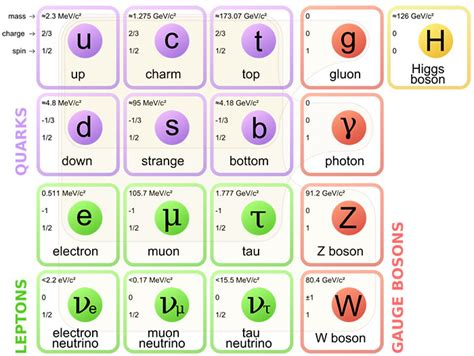
\includegraphics[width=0.5\textwidth]{standard_model.png}
When looking at phenomena outside our earth the astronomer will turn to
electromagnetic radiation, but he's missing out on a big part of the full
picture. Not only do interesting events emit photons but also muons, nuclei,
gravitational waves,... All kinds of particles which might also be of interest,
that's where the astroparticle physicist comes in.

Of all these particles there is one particle which has properties we're quite
interested in: the neutrino.  Neutrinos don't have any charge, meaning that
they are not deflected by magnetic fields. Also neutrinos interact very weakly,
because of this they are often called “ghost” particles; on average 100
trillion neutrinos pass through your body per second, none of them having any
effect.  You'd even need a light year of lead to give you just a 50\% chance of
stopping a neutrino.
These properties makes them ideal messenger particles as, when we detect a neutrino
and it's arrival direction, we can be quite sure it came to our detector unhindered
from a far away event in the exact same direction.
Neutrinos can serve as unique clues
about what’s happening elsewhere in the universe including the cosmic
collisions, galaxies, supernovae, Gamma-ray bursts (GRBs),... where they are created.

\section{Discovery}
When researching $\beta^-$ decay, the decay of a neutron, researcher
detected a proton and an electron coming from the neutron. However
on closer inspection it became apparent that energy was lost
somewhere in violation with the conservation law of energy, and
angular momentum wasn't conserved.  The solution postulated by
Wolfgang Pauli was to introduce a new, really hard to detect
particle with no charge and a very small mass: the neutrino.  The neutrino comes in three flavours:
electron, muon and tau neutrinos, each corresponding to their respective lepton denoted as
\begin{equation}
	\nu_e \quad \nu_\mu \quad \nu_\tau
\end{equation}
and each also having an anti-particle.
\begin{equation}
	\bar{\nu}_e \quad \bar{\nu}_\mu \quad \bar{\nu}_\tau
\end{equation}

Now with the introduction of the neutrino the full $\beta^-$ decay
becomes
\begin{equation}
	n \rightarrow p^+ + e^- + \nu_e
\end{equation}
The inverse can then also be used to detect neutrinos:
\begin{equation}
	n \rightarrow p^+ + e^- + \nu_e
\end{equation}
Which is called beta capture and was first experimentally detected in 1956
\cite{BetaCapture} also making it the first experimental detection of a
neutrino.
\section{Neutrino sources}
As shown in figure \ref{figure:Neutrino fluxes} there are various kinds of
neutrino sources, we'll discuss these one by one in order leaving out the
reactor anti-neutrinos and the terrestrial anti-neutrinos as we're only
interested in neutrinos of astrophysical nature.
\begin{figure}
	\centering
	\copyrightbox[r]{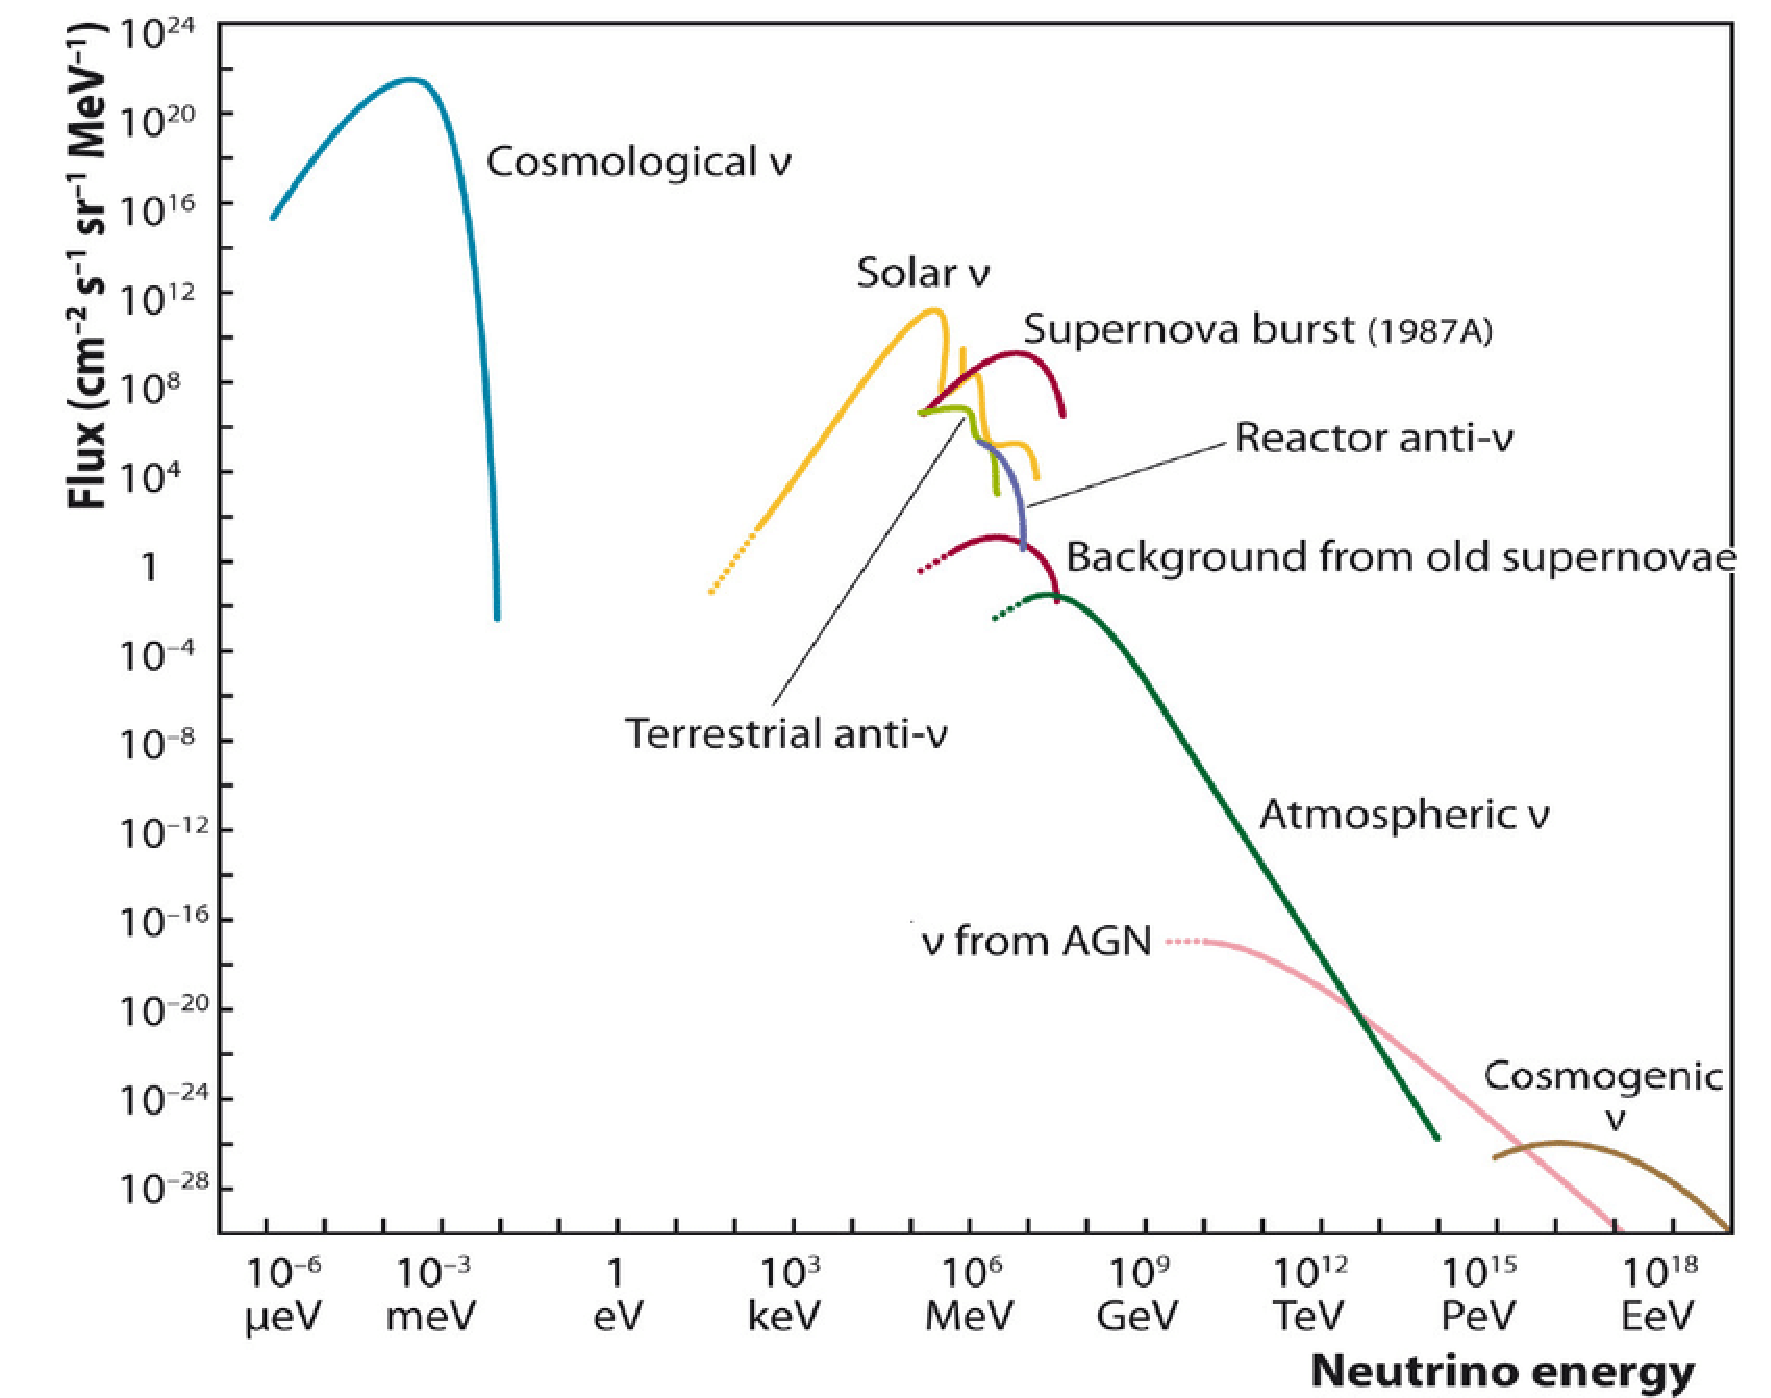
\includegraphics[height = 0.5\textwidth]{neutrinofluxes.pdf}}{\textcopyright Abhik Jash, Studies on the Physics of Resistive Plate Chambers in Relation to the INO Experiment}
	\caption{Predicted neutrino flux for various sources both natural and man-made}
	\label{figure:Neutrino fluxes}
\end{figure}
\subsection{Cosmological/Primordial neutrinos}
The first source of neutrinos we'll talk about is the one in blue to the left of the figure
termed the \textit{Cosmological neutrinos}: 
the neutrino version of the CMB.
To understand this source we'll have to go back all the way to just after the big bang:
The very early universe was hot and dense. As a result, interactions among particles
occurred much more frequently than they do today. As an example, a photon today
can travel across the observable universe without deflection or capture, so it has a
mean free path greater than $10^{26}$ m. When the universe was 1 second old, though, 
the mean free path of a photon was about the size of an atom. Thus in
the time it took the universe to expand by a factor of 2, a given photon interacted
many, many times. These multiple interactions kept the consitituents in the universe
in thermal equilibrium. But as the universe expanded there were times when reactions could
not proceed rapidly enough to maintain equilibrium conditions, these particles then fall out
of thermal equilibrium. This falling out of equilibrium is termed \textit{decoupling}.
And we're interested in when neutrinos decoupled.
Neutrinos were kept in equilibrium through the interaction 
\begin{equation}
	\nu e \leftrightarrow \nu e
\end{equation}
up until the universe cooled down to about 1MeV when they decoupled.
To estimate the temperature of the neutrinos who decoupled at the start of the universe, 
we can take a look at conservation of entropy \cite{Dodelson} from which we'll find that:
\begin{equation}
	T_\nu = \left(\frac{4}{11}\right)^{1/3}T_\gamma
\end{equation}
Note that they decoupled before the photons making them lower in temperature.
As $T_\gamma$ is the CMB temperature which, nowadays, is measured to be around
2.7K or $2.3\times10^{-4}$. This would imply $T_\nu = 1.66\times 10^{-4}$ which
is rougly where the peak flux is located.  these primordial neutrinos are thus very
low in energy.
\subsection{Solar neutrinos}
The sun fuses elements to release energy and thus keeping itself from collapsing in 
on itself, with most of the various ways particles get fused, neutrinos get released as 
is shown in figure \ref{fig:SunFusion}.
\begin{figure}
	\centering
	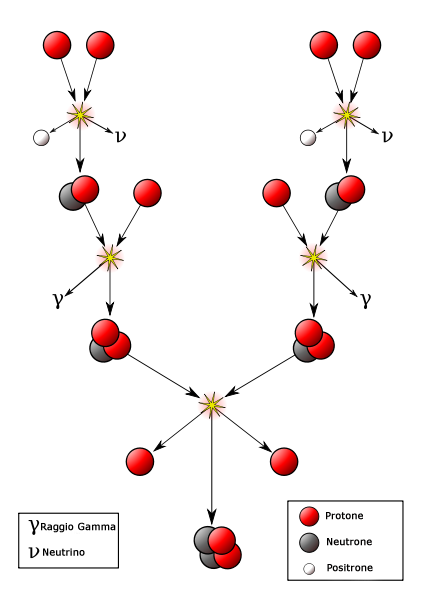
\includegraphics[width=0.4\textwidth]{figures/SunFusion.png}
	\label{fig:SunFusion}
\end{figure}
Now with this and some information about the sun like the pressure and mass,
the so-called "standard solar model" was made. This model predicted a certain
amount of neutrinos to be hitting the earth from the previously mentioned
thermonuclear fusion, it was however 3 times higher than the observed amount of
neutrinos back at our planet. This led to a little bit of hysteria as this could've meant
that the sun was dying and we'd see the aftermath only in a couple of years.
Through various experiments however, it became apparent that this was due to
the different kinds of neutrinos oscillating into each other on their way to
earth, i.e 2/3 of the original electron neutrinos had oscillated into mu and
tau neutrinos. But for them to oscillate into eachother, they not
only require mass but each flavor also should have a different mass as can be seen
from an example 2D approximation to the transition probability:
\begin{equation}
	P(\nu_e\rightarrow\nu_\mu) = |\braket{\nu_\mu|\psi(L,T)}|^2 = c_\mu c_\mu^* = \sin ^2(2 \theta) \sin ^2\left(\frac{\Delta \phi_{12}}{2}\right)
\end{equation}
with
\begin{equation}
	\Delta \phi_{12} \approx \frac{m_1^2 - m_2^2}{2p}L
\end{equation}
In full generality (3D):
\begin{equation}
	\ket{\nu_\alpha} = \sum_iU_{\alpha i} \ket{\nu_i}
\end{equation}
With $U_{\alpha i}$ the Pontecorvo-Maki-Nakagawa-Sakata (PMNS) matrix. 
This phenomenon has been observed e.g through the descrepency from the observed
and expected neutrino events coming from a nuclear reactor \cite{Eguchi_2003}.
\subsection{Supernovae}
\label{sec:supernovae}
A star starts its life as a ball of pure hydrogen. At the core, due to the
gravitational pressure of the outside plasma, fusion of hydrogen into deuterium
and helium happens. Thus converting mass into energy. The pressure of this energy
counteracts the pressure of gravity and the star is stable.

When the hydrogen at the core runs out no more hydrogen can be fused. For
stars with masses between $8M_\odot$ and $30M_\odot$ the
fusion of heavier elements starts, this can't keep going on however as at some
point the star starts to form the most stable element: iron. 
\begin{figure}[!ht]
	\centering
	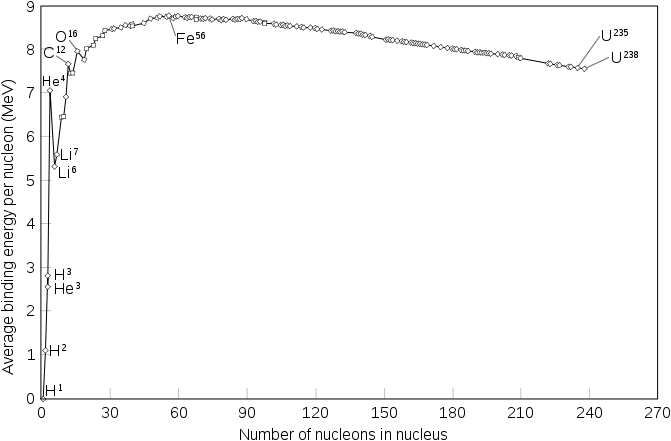
\includegraphics[width=0.5\textwidth]{Binding_energy_curve.png}
	\caption{Energy per nucleon i.f.o number of nucleons in the nucleus}
	\label{fig:BindingEnergyCurve}
\end{figure}
It costs energy
to both make lighter elements than iron and heavier ones.  As the iron core
builds up the outside pressure from the core starts to decrease as no new
energy is released. This goes on until  the treshold of an iron core with a mass of 1.4$M_\odot$ known as the 
Chandrasekhar limit is reached and the the inwards pressure becomes too large,
making the electrons surrounding the iron core fuse with the protons (uud),
creating neutrons (udd) and neutrinos, diagramatically shown in figure
\ref{fig:CoreFusion}.
\begin{figure}
	\centering
	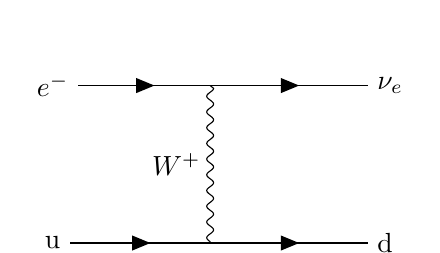
\begin{tikzpicture}
	\begin{feynman}
	\vertex (a0){u};
	\vertex[right=2cm of a0] (am) ;
	\vertex[right=2cm of am] (a1) {d};
	\vertex[above=2cm of am] (bm);
	\vertex[above=2cm of a0] (b0){$e^-$};
	\vertex[right=2cm of bm] (b1){$\nu_e$};
	\diagram* {
		{[edges=fermion]
			(a0) -- (am) -- (a1)
		},
		{[edges=fermion]
			(b0) -- (bm) -- (b1)
		},
		{[edges=boson,edge label=$W^+$]
			(am) -- (bm)
		}
	};
	\end{feynman}
	\end{tikzpicture}
	\caption{fusion of protons with surrounding electrons into neutrons via the weak force}
	\label{fig:CoreFusion}
\end{figure}\\
This last part happens in a split second as the collapse goes at 25\% the speed
of light, creating a very dense neutron star (3000km in diameter iron core to
30km in diameter neutron star) and up to $10^{52}$ ultra-relativistic
neutrinos, carrying up to 99\%\footnote{$\approx$1\% is released as kinetic energy, only 0.001\% as
electromagnetic radiation} of the released energy
\cite{Melson_2015}. As the density has suddenly increased so much
there's a huge distance of pure vaccuum between the plasma outer layer and the
(now) neutron star, this plasma starts free-falling inwards, also at 25\% the
speed of light whilst the neutrinos carrying tremendous amounts of energy start
going outwards from the neutron stars core.

The neutrinos then collide with the plasma resulting in what we observe as a
"supernova", wrongly thought of by Kepler as being a "new (nova) star" rather
being a violent death of an old star.

This is quite unexpected as neutrinos rarely interact, it's only as the
incoming plasma is so dense and due to the tremendous amount of neutrinos that
collissions happen at all. Some, however, escape and will be visible on earth
in our neutrino detectors $\approx$ 18h before the light escapes the exploding
star.

Neutrino observatories are thus also useful to know where to point our various
telescopes before the supernova is actually visible in the night sky.
\subsection{Background from old supernovae}
Also termed the \textit{diffuse supernova neutrino background} (DSNB), as the
universe is quite old various supernovae have happened over it's lifetime, each generating
a lot of neutrinos as was discussed in section \ref{sec:supernovae}. 
This is postulated to have generated a continuous neutrino background.
\subsection{Atmospheric neutrinos}
\label{sec:AtmosphericNeutrinos}
Before we can talk about atmospheric neutrinos it's necessary to discuss \textit{cosmic rays}.
Cosmic rays are ionized nuclei of which 90\% are protons, 9\% are alpha particles and
the rest are heavier nuclei. Almost all of them originate from outside the solar system but
from within our galaxy, the few particles that do come from our solar system can be temporally
linked to violent events on the sun. In contrast to this the particles coming from outside
our solar system show an anti-correlation with the sun as they can more easily reach the earth
if solar activity is low.
It has been observed that they roughly follow a power-law spectrum 
$N \propto E^{-\gamma}$ \cite{gaisser_engel_resconi_2016}.

Cosmic rays hit the Earth's atmosphere at a rate of about 1000 per square meter
per second and interact with atomic nuclei in the Earth's atmosphere, creating
showers of particles, many of which are unstable and produce neutrinos when
they decay, these neutrinos are what's called \textit{Atmospheric neutrinos}.
Most notably neutrinos can be produced together with muons in the two-body
decays of charged pions and kaons wherever these hadronic interactions occur.
The most important production channels and their branching ratios for neutrinos
are:
\begin{align}
	\pi^\pm &\rightarrow \mu^\pm + \nu_\mu(\bar{\nu}_\mu) (\sim 100\%)\\
	K^\pm &\rightarrow \mu^\pm + \nu_\mu(\bar{\nu}_\mu) (\sim 63.5\%)
\end{align}
Neutrinos are subsequently also produced when these muons decay:
\begin{equation}
	\mu^\pm \rightarrow e^\pm + \nu_e(\bar{\nu}_e) + \bar{\nu}_\mu(\nu_\mu)
\end{equation}
which is a process mainly happening at low energies in the atmosphere.  The
atmospheric neutrino spectrum shown in figure \ref{figure:Neutrino
fluxes} roughly follows a power spectrum as the cosmic ray flux follows a power
spectrum but the correspondence isn't one-to-one as, due to the difference in
kinematics, the contribution from kaons to neutrinos is significantly more
important than to muons, especially at high energies.

\subsection{neutrinos from AGNs}
An AGN (active galactic nucleus) is deemed to be the reason why several abnormal galaxies exist with
an extra bright (and mostly variable) light source in their core which even the biggest of telescopes
can't spatially discern. The general concensus is that this phenomenon is caused by one particular
kind of object: a supermassive black hole (a black hole with a mass of at least 105M$_\odot$) surrounded with
a close torus of dust and gas.
This torus of gas is called an \textit{accretion disc} and is an enormous source of energy. The conversion
of potential energy of the incoming gas to highly energetic radiation is a very complex physical process
with which we have to account for various factors like gravitational instabilities, magnetic fields, hydrodynamical
turbulence,... And thus produces a spectrum that's quite complex.
It would appear that the luminocity of an AGN would increase indefinitely with incoming mass, but this process is 
limited: if too much matter accretes on the black hole the radiative pressure becomes too massive and the 
matter on the disc gets blown away, this phenomenon is termed a \textit{black hole outburst}.

The emission of high energy neutrinos from AGNs rests solely on the premise
that relativistic protons of sufficiently high energy and energy density in the
AGN's accretion disc will be present \cite{NASANeutrinos} as they may interact
to create e.g pions whom decay. A direct consequence of the occurence of these
relativistic protons is the production of $\gamma$-rays of similar energies to
those of the neutrinos, thus high energy neutrino- and $\gamma$-ray astronomy are
closely related.  However, even though $\gamma$-ray photons can be produced
even in the absence of relativistic protons (e.g via high energy electrons),
neutrinos can not.  Thus the detection of these high-energy neutrinos (which
might have already been detected \cite{AGNNeutrino}) will provide unique
information about the workings of AGNs.
As these ultra high energy neutrinos get produced near the source (the AGN)
they are what's called \textit{astrophysical neutrinos}

\subsection{Cosmogenic neutrinos}
In contrast to the previous source of UHE neutrinos which was generated at the
source, called \textit{astrophysical neutrinos} we'll now talk about UHE
neutrinos whom are generated through the interaction of ultra-high energy
cosmic rays during propagation with the cosmic microwave or other photon
backgrounds termed \textit{cosmogenic neutrinos}.  The mechanism by which these
get created is quite simple, if a proton has sufficiently high energy the cross
section to interact with CMB (Cosmic Microwave Background) photons becomes
non-negligable.  These protons can scatter off the photons to resonantly
produce a $\Delta^+$ baryon.  This resonance has enough mass to dominantly
decay to a pion and a nucleon:
\begin{align}
	\Delta^+ &\rightarrow \pi^0 + p \ \ (2/3)\\
	\Delta^+ &\rightarrow \pi^+ + n \ (1/3)
\end{align}
Of which the charged pion decays to neutrinos as previously mentioned in 
\ref{sec:AtmosphericNeutrinos}.
\subsection{How do they fit into the full detector spectrum?}
The origin of the most energetic cosmic rays is still not conclusively
identified. One approach to solving this problem is \textit{multi-messenger
astrophysics}, where several types of cosmic particles are used to identify the
sources of these ultra-high energy cosmic rays (UHECRs). E.g we simultaneously
measure gravitational waves with the Einstein telescope, neutrinos with RNO-G,
photons with various telescopes and muons with a muon detector.
\newpage
\section{Current research}
Talk about first IceCUBE something?
\newpage
\chapter{Radio detection of neutrinos}
\section{Neutrino interactions in ice}
As neutrinos propagate through ice they can interact weakly. The main
mechanisms of interaction is by charged (W boson) and neutral current (Z boson)
exchange with nuclei \cite{NuRadioMc} as is also depicted in figure
\ref{fig:NeutrinoNucleusInteraction}.
\begin{figure}[h!]
	\begin{minipage}{\textwidth}
		\begin{minipage}{0.49\textwidth}
			\centering
			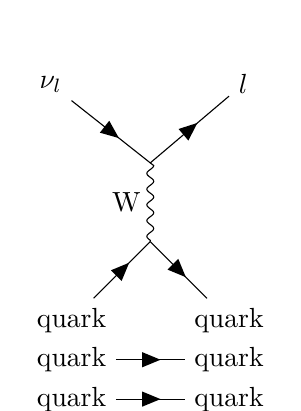
\begin{tikzpicture}
				\begin{feynman}
					\vertex (a0) {quark};
					\vertex[above=0.5cm of a0] (a1) {quark};
					\vertex[above=0.5cm of a1] (a2) {quark};
					\vertex[right=2cm of a0] (b0) {quark};
					\vertex[right=2cm of a1] (b1) {quark};
					\vertex[right=2cm of a2] (b2) {quark};
					\vertex[right=1.0cm of a2] (am);
					\vertex[above=1cm of am] (c0);
					\vertex[above=1cm of c0] (c1);
					\vertex[above=1cm of c1] (cm);
					\vertex[left=1cm of cm] (a3) {$\nu_l$};
					\vertex[right=1cm of cm] (b3) {$l$};
					\diagram* {
						{[edges=fermion]
							(a0) -- (b0)
						},
						{[edges=fermion]
							(a1) -- (b1)
						},
						{[edges=fermion]
							(a2) -- (c0) -- (b2)
						},
						{[edges=fermion]
							(a3) -- (c1) -- (b3)
						},
						{[edges=boson, edge label=W]
							(c0) -- (c1)
						},
					};
				\end{feynman}
			\end{tikzpicture}
		\end{minipage}
		\begin{minipage}{0.49\textwidth}
			\centering
			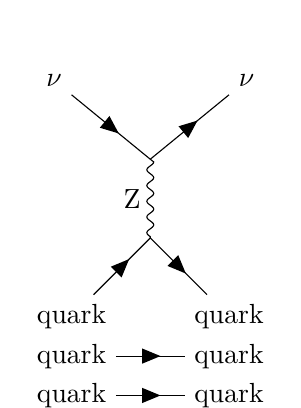
\begin{tikzpicture}
				\begin{feynman}
					\vertex (a0) {quark};
					\vertex[above=0.5cm of a0] (a1) {quark};
					\vertex[above=0.5cm of a1] (a2) {quark};
					\vertex[right=2cm of a0] (b0) {quark};
					\vertex[right=2cm of a1] (b1) {quark};
					\vertex[right=2cm of a2] (b2) {quark};
					\vertex[right=1.0cm of a2] (am);
					\vertex[above=1cm of am] (c0);
					\vertex[above=1cm of c0] (c1);
					\vertex[above=1cm of c1] (cm);
					\vertex[left=1cm of cm] (a3) {$\nu$};
					\vertex[right=1cm of cm] (b3) {$\nu$};
					\diagram* {
						{[edges=fermion]
							(a0) -- (b0)
						},
						{[edges=fermion]
							(a1) -- (b1)
						},
						{[edges=fermion]
							(a2) -- (c0) -- (b2)
						},
						{[edges=fermion]
							(a3) -- (c1) -- (b3)
						},
						{[edges=boson, edge label=Z]
							(c0) -- (c1)
						},
					};
				\end{feynman}
			\end{tikzpicture}
		\end{minipage}
	\end{minipage}
	\caption{Most prominent ways of neutrino-nucleus interaction}
	\label{fig:NeutrinoNucleusInteraction}
\end{figure}\\
With the produced leptons in the W boson mediated interaction being either electrons,
resulting in an electromagnetic shower, muons wich typically go undetected as they live
too long or
tauons wich will decay via
\begin{equation}
	\tau^- \rightarrow e^- + \bar{\nu}_e + \nu_\tau
\end{equation}
or, less ideally
\begin{equation}
	\tau^- \rightarrow \mu^- + \bar{\nu}_\mu + \nu_\tau
\end{equation}
In both of the possible interactions (W or Z exchange) the resulting nucleus
will result in an hadronic shower, for the neutral current interaction (mediated
by the Z boson) the fraction of the neutrino energy that gets transferred to
the nucleon is described by the inelasticity $y$ and is heavily shifted towards
small values of $y$\cite{elasticity_y}. This causes a big, irreducable
uncertainty when trying to estimate the original neutrino energy from these
kinds of events.  With the charged current interaction (mediated by the $W^\pm$
bosons) this isn't a problem however as the full neutrino energy ends up in the
resulting cascades.
\section{Askaryan effect}
For a particle shower to emit strong radio signals, two conditions have to be met:
\begin{itemize}
	\item There needs to be a separation of positive and negative charges in the shower front 
	\item The signals produced over the length of the shower profile need to overlap coherently.
\end{itemize}
The \textit{Askaryan} \cite{Askaryan} effect, which is responsible for the
production of Askaryan radiation describes the effect at radio frequencies
which abides by both of these conditions. 
In general it's a quite difficult effect but we'll give a crude overview.  The previously described interactions
create a shower of secondary charged particles containing a charge anisotropy.
This charge imbalance is a result of medium electrons either Compton scattering
into the advancing shower or annihilating with shower positrons.  In the end
you have a moving charge anisotropy, propagating faster than the speed of light
in the medium, creating Cherenkov radiation.  

Cherenkov radiation is like the electromagnetic equivalent of a sonic boom, a
sonic boom happens when something goes faster than the speed of sound in the
medium; A particle emits Cherenkov radiation if it goes faster than the speed
of light in the medium\footnote{The reader who wants a thorough explanation and
derivation is advised to check out \textit{Chapter 14: Radiation by Moving
Charges} from the book \textit{Classical Electrodynamics} by Jackson.} .
Choosing the particle trajectory to lie along the z axis an approximate
equation can be found\cite{jackson1998classical} for $\frac{\text{d}^2
\mathscr{J}}{\text{d}\omega \text{d}\Omega}$: the energy radiated per
elementary unit solid angle and per elementary unit frequency interval
\begin{equation}
	\frac{\text{d}^2 \mathscr{J}(\omega)}{\text{d} \omega \text{d} \Omega} = \frac{q^2}{4\pi}\sqrt{\frac{\mu}{\epsilon}}\beta^2\omega^2\delta^2[\omega(1-\beta \mathbf{e}_r\cdot\mathbf{e}_z)]|\mathbf{e}_r\times\mathbf{e}_z|^2 \label{equation: 4.128 in elektromagnetisme}
\end{equation}
Now we can re-write this equation in spherical coordinates, which gives $1-\beta \mathbf{e}_r\cdot\mathbf{e}_z = 1-\beta\cos(\theta_c)$ in the delta function. We thus only expect radiation if
\begin{equation}
\cos(\theta_c) = \frac{1}{\beta} = \frac{c'}{u} = \frac{c}{n}\cdot\frac{1}{u}
\end{equation}
With u the local speed of light in the medium and n the index of refraction.
I.e if $u>\frac{c}{n}$, Cherenkov radiation will
be emitted along a cone surface with half angle $\frac{\pi}{2}-\theta_c$ as
illustrated in figure \ref{figure: Cherenkov illustratie}. Integrating equation
\ref{equation: 4.128 in elektromagnetisme} over the solid angle and formally
dividing by the time interval we get:
\begin{equation}
	\frac{\text{d}^2\mathscr{J}}{\text{d}\omega \text{d}t} = \frac{q^2}{4\pi}\sqrt{\frac{\mu}{\epsilon}}\beta\omega\left(1-\frac{1}{\beta^2}\right)	
\end{equation}
We see that the energy is proportional to $\omega$, so we expect that most
radiation will be emitted "in blue" with a cut-off frequency above which the
equation $\cos\theta = 1/(n\beta)$ can no longer be satisfied, this "in blue"
characteristic is responsible for the blue glow seen in nuclear reactors as
seen in figure \ref{figure: Cherenkov reactor} .  For ice the index of
refraction is roughly 1.78 in deep ice, so we expect an ultra-relativistic
particle to produce the most radiation at around 56° opening as 
\begin{equation}
	\cos(\theta_c) \approx \frac{1}{n} \implies \cos^{-1}\left(\frac{1}{1.78}\right)\approx 56\text{°}
\end{equation}
\begin{figure}
\centering
\begin{minipage}{0.45\textwidth}
	\centering
	\copyrightbox[r]{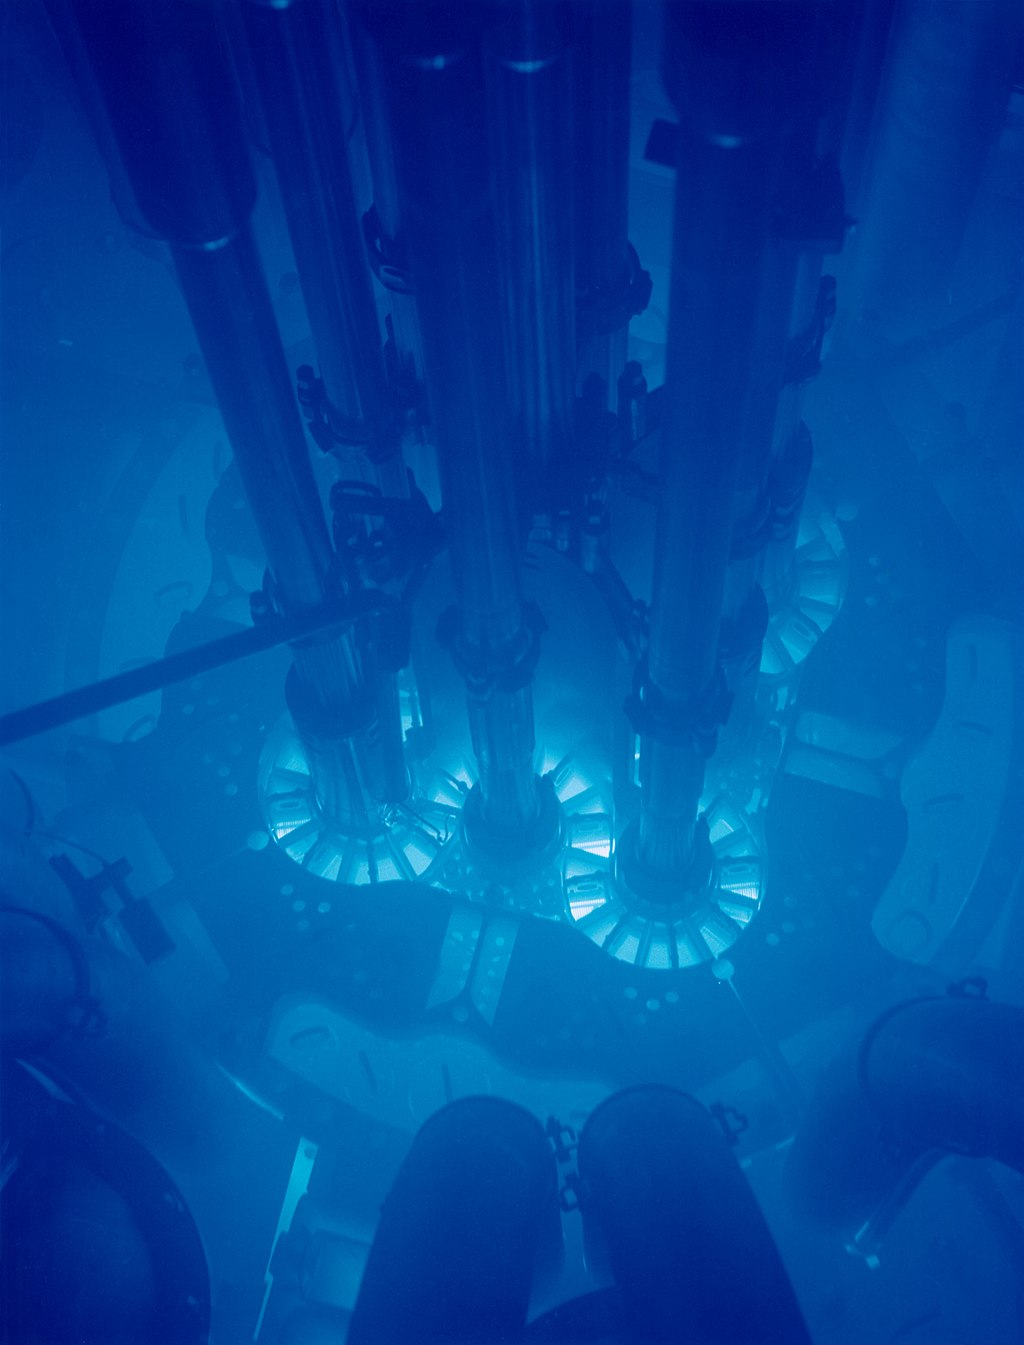
\includegraphics[height = 0.8\textwidth]{Cherenkov-reactor.jpg}}{\textcopyright Argonne National Laboratory\\Advanced Test Reactor core, Idaho National Laboratory}
	\caption{Cherenkov radiation in a nuclear reactor}
	\label{figure: Cherenkov reactor}
\end{minipage}
\hspace{0.05\textwidth}
\begin{minipage}{0.45\textwidth}
	\centering
	\copyrightbox[r]{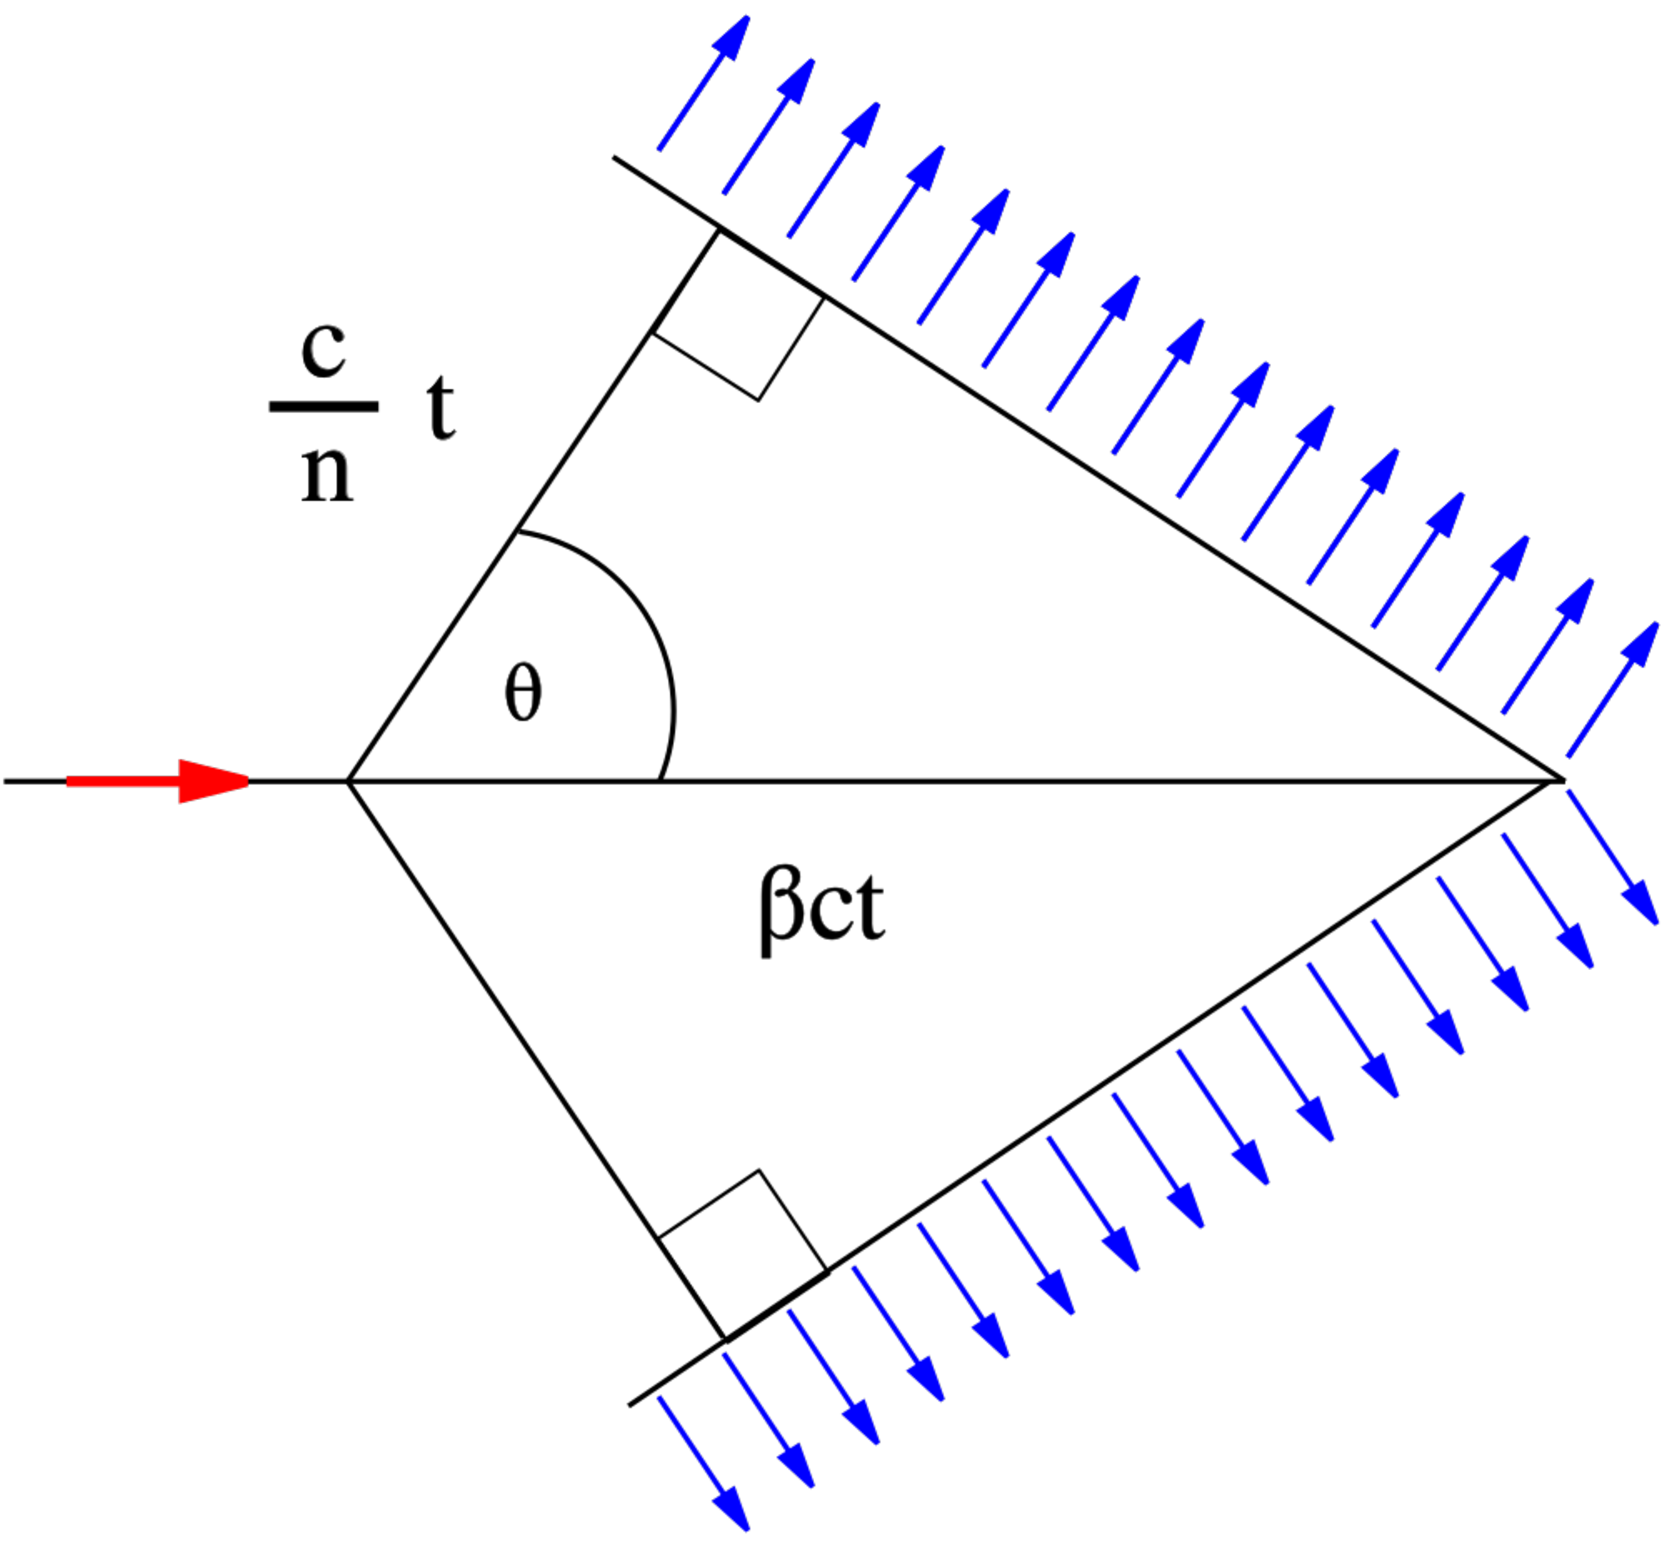
\includegraphics[height = 0.8\textwidth]{Cherenkov.pdf}}{\textcopyright Arpad Horvath}
	\caption{Diagrammatic representation of Cherenkov radiation}
	\label{figure: Cherenkov illustratie}
\end{minipage}
\end{figure}
Of course this is just an estimate, as the actual index of refraction is depth-dependent which
we'll get to in section \ref{section:Ice Model}.
Now this explains how the signals get generated but logically, from only knowing this
we'd expect radio waves to almost be non-existent 
due to the "in blue" nature of Cherenkov radiation. 
This isn't the full story however as we'll need to talk about coherent overlap
to fully understand the Askaryan effect. This can be intuitively explained as
follows: generally the shower is of length
$\mathcal{O}$(10cm)\cite{Huege_2017}, over this length the radiation gets
emitted, most frequencies decoherently interfering, but radio waves with wavelengths of 
$\approx$ 10cm coherently interfere, and it's these waves we then wish to detect.


The generated electromagnetic radiation is polarized perpendicular to the
cherenkov cone, this can be useful to discern between different cherenkov cones whom,
timely, would generate the same response. This concept is illustrated below in 2D where
two neutrinos from different directions would generate the same signal in the detector.
If the detector has a way to differentiate between polarization however, there would be no
doubt where the neutrino originated from as the one producing the yellow cherenkov cone
would have a downwards polarization and the one producing a green cherenkov cone would have
an upwards polarization, note that in 3D infinite different cherenkov cones could generate
the same timely signal (think of rotating the cone around a line on the cone) so both vertical
and horizontal polarization information is needed.

\begin{figure}[h!]
	\centering
	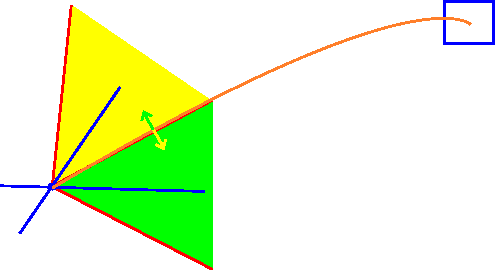
\includegraphics[width=0.5\textwidth]{illu_polarization.pdf}
\end{figure}
\section{Wave propagation}
\begin{figure}[h!]
	\centering
	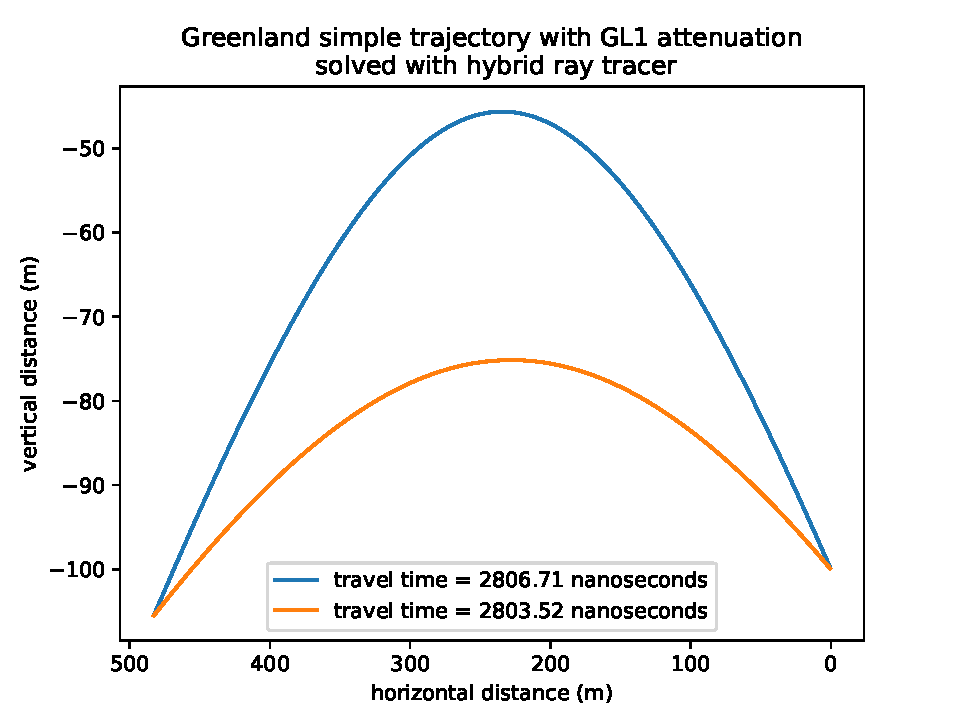
\includegraphics[width=0.7\textwidth]{path_illustration.pdf}
	\label{fig:PathIllu}
	\caption{illustration of radiowave paths generated by a neutrino event}
\end{figure}
The way we simulate the strongest waves propagating to the detector from a
radio source is through ray tracing, an illustration of such a simulation is
shown in figure \ref{fig:PathIllu}.  Here the detector is located at (0,-100)
and a radio source at (480,-108), note that there are two possible paths
leading to the detector.

The amount of solutions and how the waves are bent is due to the nature of the
ice we work in.  In a dielectric medium a ray propagates with it's signal
wave-speed determined by the local index of refraction as $v = c/n$.   The
effect on speed isn't the only effect the index of refraction has which we'll
need to concern ourselves with however, if a ray propagates towards a boundary
dividing 2 media with different indexes of refraction, the ray will refract and
the refracted angle can be found from Snell's law:
\begin{equation}
	n_i\sin{\theta_i} = n_o\sin{\theta_o}
\end{equation}
Where n is the index of refraction, $\theta$ the angle with respect to the
surface normal and "i" and "o" indicating incoming and outgoing respectively.
The system we'll consider however, isn't homogeneous with some specified
boundary, it's continous: ice in greenland has a continously varying density and
index of refraction.

How do we know how the waves propagate in a medium?  The software we'll be
using to simulate how the radio waves behave is called \textit{Radiopropa}
\cite{Winchen_2019} and as  simulations of the wave propagation in full detail
with the finite-differences-time-domain (FDTD) technique \cite{1138693} are,
even though they are more accurate, too time consuming. Have the authors of
radiopropa chosen to build their program on geometrical optics, i.e ray
tracing. A path of a ray $\mathbf{r}(s)$ with path parameter s in a medium
with index of refraction n($\mathbf{r}$) is described by the eikonal
equation\cite{herman2019treatise}:
\begin{equation}
	\frac{d}{ds}\left(n(\mathbf{r})\frac{d\mathbf{r}}{ds}\right) = \mathbf{\nabla} n
\end{equation}
in radiopropa the local paraxial approximation (small angle approximation) is
used, i.e if we assume that in any individual step of the algorithm the change
of the refractive index along the path ds is small it's possible to re-write
the equation as:
\begin{equation}
	n(\mathbf{r})\frac{d^2\mathbf{r}}{ds^2} \approx \mathbf{\nabla} n
	\label{eqn:radiopropaformula}
\end{equation}
Which is then iteratively solved using the Cash–Karp method.  The way you would
go about using this program is thus find a start and end point (e.g a supposed
neutrino interaction point and a detector respectively), "shoot" your ray in a
certain direction for which the path will then be iteratively solved using
radiopropa and if you chose your direction right you have the path a ray might
take from your start to the end point.  The big complication is this direction
choosing which we'll get to later.  If there are boundaries (such as defects or
the surface) these are treated seperately using Snell's law. 
\section{Ice model}
\label{section:Ice Model}
Ice has a density gradient which we'll need to account for. Due to the way the
ice bonds there will be more air trapped inbetween the molecules closer to the
surface than at greater depths where the pressure due to the overhead ice
prevents this.  Due to this air being trapped the density of ice will be
smaller closer to the surface than at greater depth.  

Purely from classical gravity and density considerations it can be derived that
the density scales exponentially. To see this let's consider a sheet of ice in
the Greenland firn with a surface A and a height dz, the extra pressure this
sheet of ice exerts on the ice just below it is:
\begin{equation}
	d\sigma = \frac{dF}{A} = -\frac{gdM}{A} = -g\frac{A\rho(z)dz}{A} = -g\rho(z)dz
\end{equation}
with $\rho(z)$ the depth-dependent density. Now we can assume that in the
densification of the firm the added pressure is linearly proportional to the
change in density
\begin{align}
	d\rho &= A\rho(z)dz\\
	\frac{d\rho}{\rho} &= Adz
\end{align}
integrating the left side from $\rho_0$ to $\rho$ and the right side from 0 to z we get:
\begin{align}
ln\left(\frac{\rho}{\rho_0}\right) &= Az := z/z_0\\
	\rho = \rho_0 e^{z/z_0}
\end{align}
Now as theoretically we can't expect the density to decrease forever we add an offset:
\begin{equation}
	\label{eqn:myderiexp}
	\rho = \rho_0 e^{z/z_0} + B
\end{equation}
And we're done! Schytt did a derivation similar in nature but with a different
assumption resulting in a different equation. He assumed the proportional
change in air space to be proportional to the change in pressure:
\begin{equation}
	\frac{dV}{V} \propto d\sigma
\end{equation}
As the volume scales inversely with the density let's assume the relation $V \propto (\rho_i - \rho)$ with
$\rho_i$ the density of pure ice, this yields\cite{herron_langway_1980}:
\begin{align}
	\frac{d\rho}{\rho_i - \rho} &\propto \rho dz\\
	\frac{d\rho}{\rho(\rho_i - \rho)} &\propto \rho dz \label{eqn:SchyttEnd}\\
	\frac{\ln\left(\frac{\rho}{\rho_i-\rho}\right)}{\rho_i} + C &= Az\\
	\ln\left(\frac{\rho}{\rho_i-\rho}\right) &= A\rho_iz + C\\
	\frac{\rho}{\rho_i-\rho} &= e^{A\rho_iz + C} := Ae^{z/z_0}\\
	\rho &= \frac{A\rho_i e^{z/z_0}}{1 + Ae^{z/z_0}}
\end{align}
Note that Schytt only worked with equation \ref{herron_langway_1980}, the
further derivation was my doing.  After again adding an offset, we get:
\begin{equation}
	\rho = \frac{A\rho_i e^{z/z_0}}{1 + Ae^{z/z_0}} + B
\end{equation}
Figure \ref{fig:DensityMeasurements} shows how these functions fit the density
curve.  There is one big downside however, it seems that the ice actually
doesn't follow these exponential curves perfectly but would more closely follow
some kind of higher order function.
\begin{figure}
  \centering
	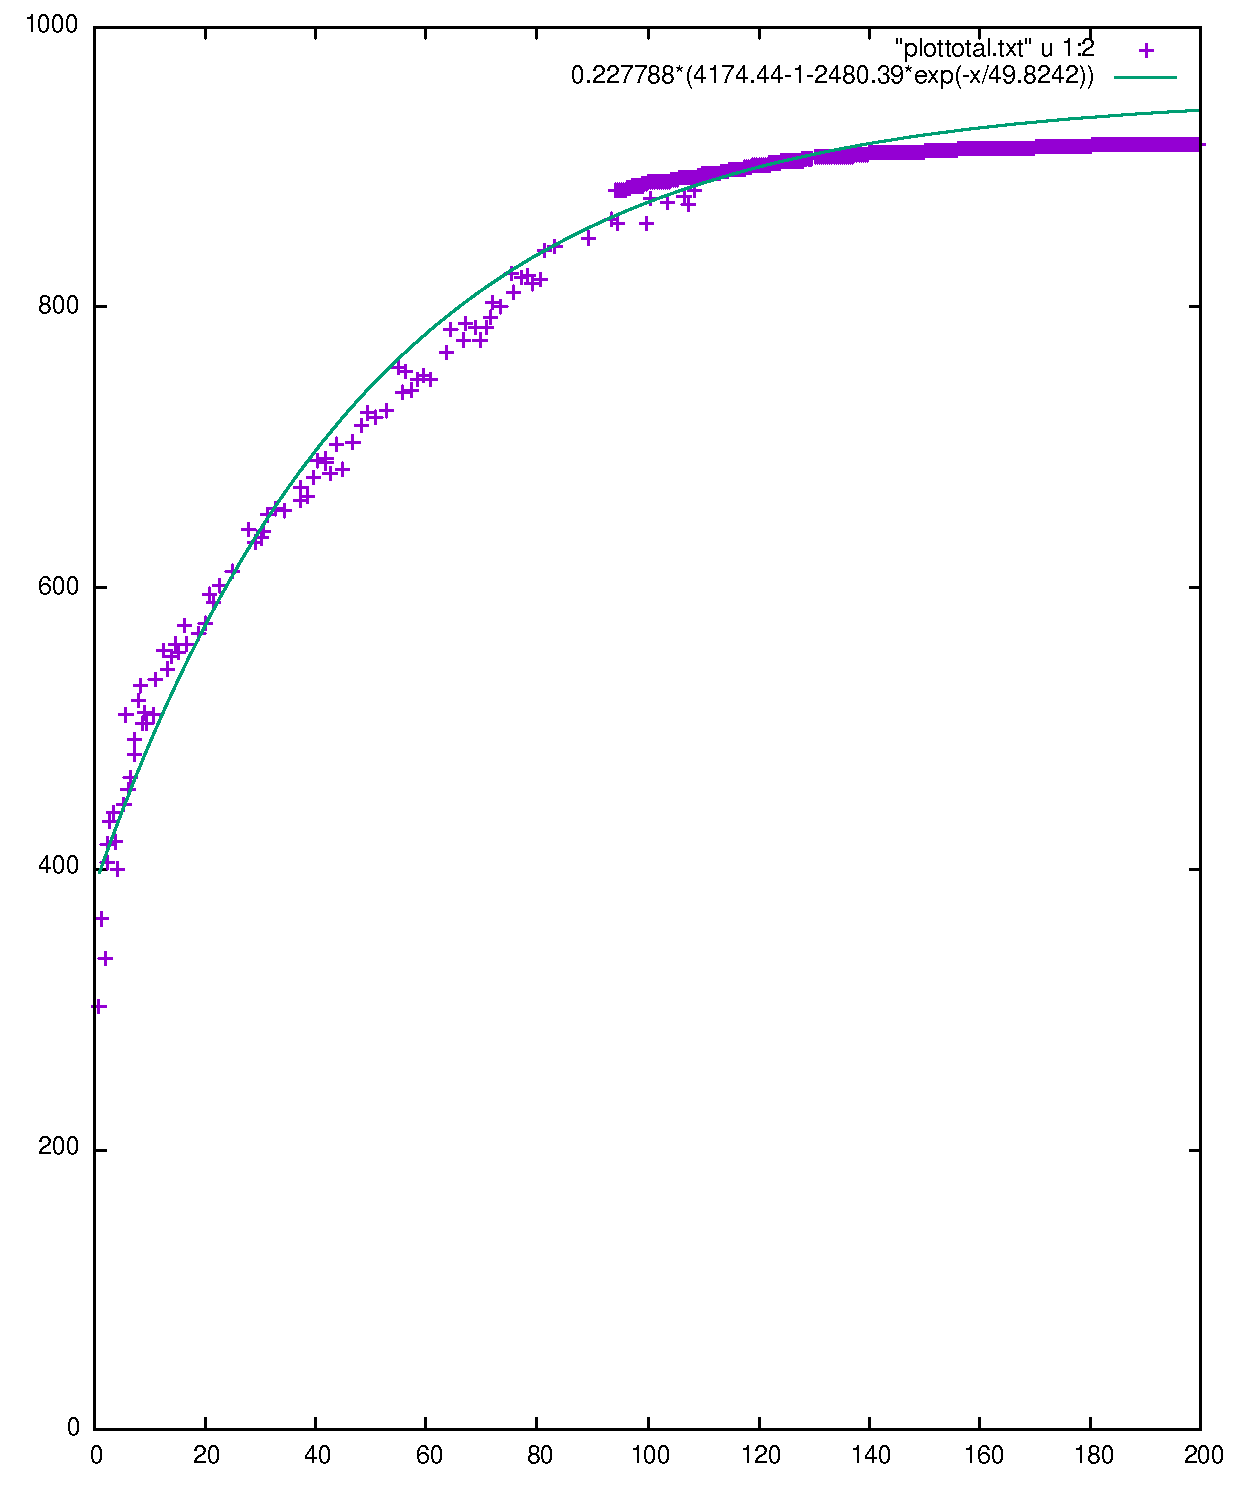
\includegraphics[width=0.5\textwidth]{Density_measurements2.pdf}
	\caption{Illustration of the shortcomings of the analitical models}
	\label{fig:DensityMeasurements}
\end{figure}

Equation \ref{eqn:radiopropaformula}, and thus the path, depends on the index
of refraction on a given location.  The dependence of the index of refraction
on density for ice can approximately be given by the Schytt equation\cite{Barwick_2018}:
\begin{equation} 
	n(x,y,z) \approx 1 + 0.78\rho(x,y,z)/\rho_0 \label{eqn:Schytt}
\end{equation} 
Where $\rho(x,y,z)$ is the local ice density and $\rho_0$ is the
density for solid ice (917 kg/m³).  For the development of the simulation
software equation \ref{eqn:myderiexp} was taken and after assuming Schytt's
equation to hold we find that the index of refraction abides by
\begin{equation}
	\label{eqn:expn}
	n(z) = n_{ice} - \Delta n e^{z/z_0}
\end{equation}
with $n_{ice}$ the refractive index of solid ice and $\Delta n = n_{ice} - n_s$
with $n_s$ the index of refraction of snow. This exponential dependency of the
index of refraction on depth is called "the single exponential model".  

This single exponential model has a huge advantage as it's analytically
solvable, meaning that we can know which direction we'll have to shoot our ray
in (as mentioned previously) after the location of the neutrino interaction and
the detector are specified, the ray tracing software developed in complience
with this exponential density profile is called the \textit{analytic ray
tracer}.

The discrepency between the single exponential model and the actual data
implies that the analytic ray tracer will make the wrong predictions.  This is
why the development of a different ray tracer was needed which will be able to
handle more complex ice models, one such ray tracer will be explained in
section \ref{sec:Iterative} but this ray tracer has it's shortcomings. That's
why the development of a new ray tracer was needed which is the partial work of
this thesis and we'll get to that ray tracer in chapter \ref{chapter:hybrid}.

Lastly there is an effect which might become important in the future:
birefringence.  Up until now have implicitly assumed that ice is isotropic
meaning that both it's permittivity $\varepsilon$ and it's permeability $\mu$
are scalars but these could very well be tensorial in nature for radio waves in
ice. In general, after calculating this tensorial nature through you'd find
that in every direction two different indices of refraction can be found
implying two different types of waves each propagating with a different speed
as illustrated in figure \ref{fig:Fresnel}. Which of the two speeds in a
certain direction is then dependent on the polarization of the wave, which in
our case thus depends on the Cherenkov cone. The optical property coming from
the anisotropic nature of the material is what's called \textit{birefringence}.
Birefringence has been extensively researched for implementation in the
simulation software NuRadioMC used in the RNO-G group \cite{Heyer2023}.

\section{Iterative ray tracer}
\label{sec:Iterative}
The iterative ray tracer \cite{2022icrc.confE1027O}, as can be derived from
it's name, iteratively searches the path a ray might take. The workings of the
first part of the explanation is illustrated in figure \ref{fig:Illustration of
iterative algorithm}.  Say we have a neutrino interaction point $\mathbf{X}_i$
(the red cross on the figure) and a detector located at $\mathbf{X}_d$ (the
blue dot on the figure), the algorithm starts by constructing an
\textit{observer} sphere with radius $r_1$ and the detector located at $\mathbf{X}_d$ at the
center.  This means that any ray that gets shot and propagates to the sphere
will get stopped ans count as a solution.  Then, to reduce the time spent simulating there's also an observer placed
just above the surface as a ray that escapes the ice won't come back and one
just behind the detector looking from the point of the interaction vertex $\mathbf{X}_i$ as
a ray is not able to reach the detector anymore after it has passed it in the
lateral direction. Finally it's noted that due to the way the ice's index of refraction
continuously increasing downwards, rays can't propagate upwards, this means that we only 
have to look for solutions within the angle $\Omega$ which is just the angle the detector
makes with the interaction vertex.
\begin{figure}
  \centering
  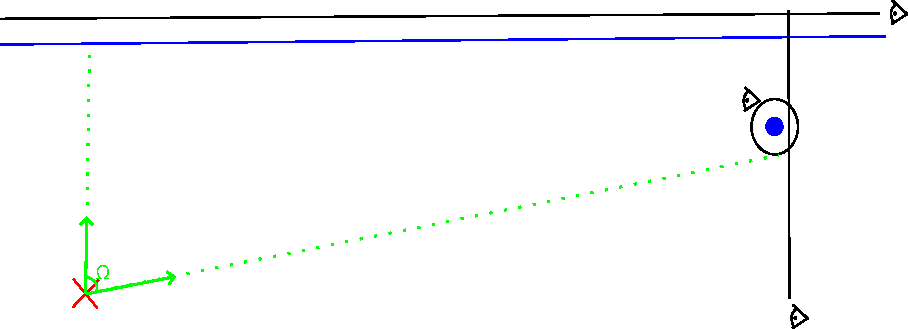
\includegraphics[width=0.7\textwidth]{algoillu.pdf}
  \caption{Illustration of the workings of the iterative algorithm}
  \label{fig:Illustration of iterative algorithm}
\end{figure}
Now that we have our setup we'll just iteratively shoot rays from
the neutrino interaction point starting at an angle $\delta \theta$ 
then at an angle $2\delta \theta$, $3\delta \theta$,... Until
we have reached $\Omega$. This process is illustrated in figure 
\begin{figure}
  \centering
  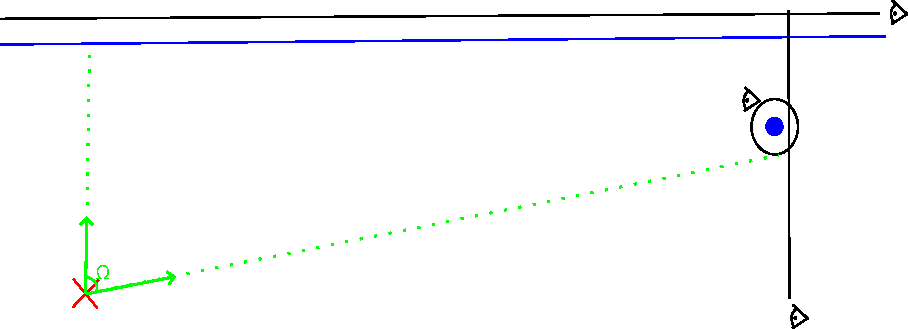
\includegraphics[width=0.7\textwidth]{algoillu.pdf}
  \caption{Illustration of the steps of the iterative ray tracer}
  \label{fig:IlluIterative}
\end{figure}

\chapter{Detector}
\begin{figure}
  \centering
  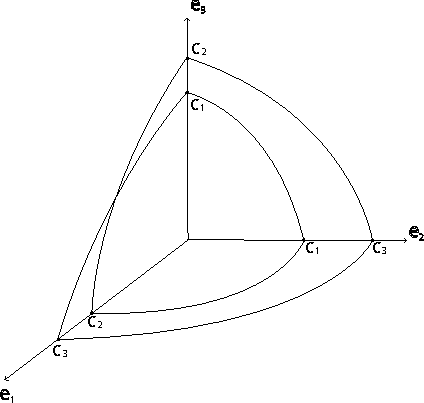
\includegraphics[width=0.5\textwidth]{figures/Fresnel.pdf}
  \caption{Wave surface of Fresnel with two sheets}
  \label{fig:Fresnel}
\end{figure}
\section{Introduction}
Both cosmic ray and neutrino detectors face the same main problem at the
highest energies: the steeply falling flux (as was previously discussed in
chapter 2) requires large effective areas, which leads to the construction of
neutrino detectors with volumes on the cubic kilometer scale: IceCube.  But
even IceCube has it's limitations, it's still too small to observe neutrino
events above the PeV scale, that's why a new detector was needed which was even
bigger.  We could just make IceCube bigger but this would cost a lot of money
as the individual detectors need to be spaced closely as IceCube works in the
visible spectrum for which the attenuation length is quite short. The proposed
solution was to work with radiowave detectors, leveraging the Askaryan effect
which has been previously explored e.g in the NuMoon project.  Besides the
advantage radiowaves have due to their abundance, they can also propagate way
further in ice than visible light making it possible to space the individual
detectors further apart. The proposed location was Greenland, an island country
in North America and part of the Kingdom of Denmark which has large ice sheets.
An orthographic projection projection of greenland is shown in figure
\ref{fig:GreenlandOP} and both Greenland's flag and it's code of arms are shown
(???) This needs to be deleted
in figure \ref{fig:FlagAndArms}, the flag sports the same colors as it's parent
country's flag Denmark. The flag is designed by Thue Christiansen who described
the white stripe as representing the glaciers and ice cap, which cover more
than 80\% of the island; the red stripe, the ocean; the red semicircle, the
sun, with its bottom part sunk in the ocean; and the white semicircle, the
icebergs and pack ice. The design is also reminiscent of the setting Sun
half-submerged below the horizon and reflected on the sea.
\begin{figure}
  \centering
  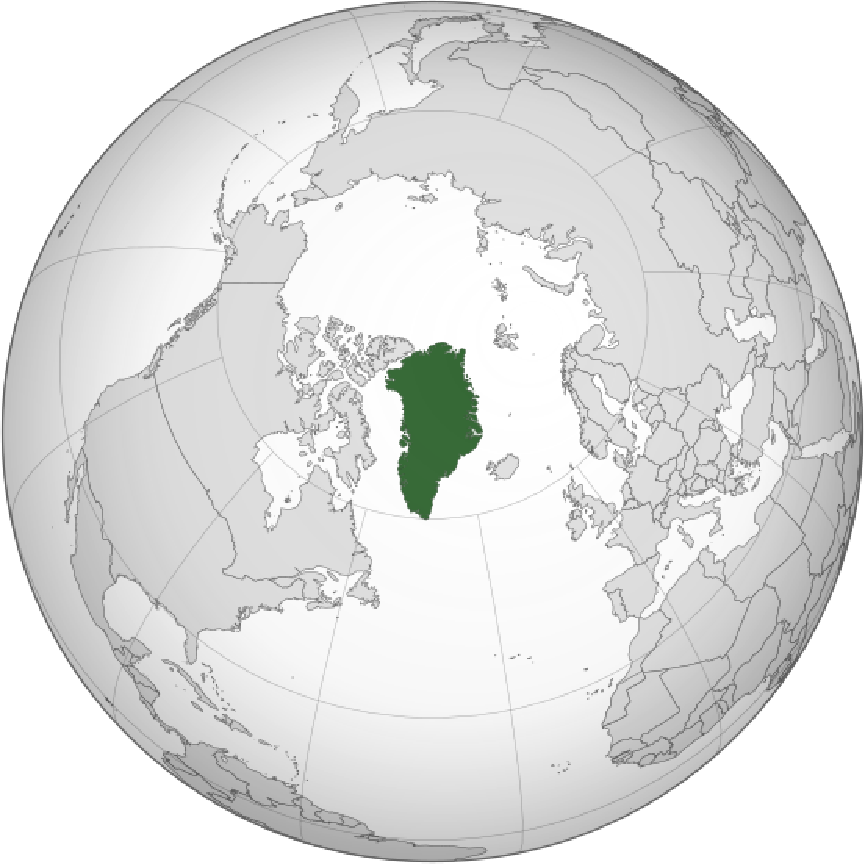
\includegraphics[width=0.5\textwidth]{figures/GreenlandOP.pdf}
  \caption{orthographic projection of Greenland}
  \label{fig:GreenlandOP}
\end{figure}
\newpage
The proposal for RNO-G, which was later funded and now in the construction
phase, is it be an array of autonomous radio stations each of which having both
surface channels and various deep channels resulting in a total of 24 channels
per station. The whole project builds heavily on the knowledge obtained through
previous neutrino detectors like ARA, RICE and ARIANNA experiments, as well as
the balloon-borne ANITA experiment.
\section{Hardware}
One such detector is illustrated in figure \ref{fig:detector}, the plan is to
build 35 of these as is shown in figure \ref{fig:station map}\footnote{note
that all the individual detectors are named after various species living in
greenland (in the native tongue)}. Looking closely at one such detector we see
just below the surface 9 Log Periodic Dipole Antennas (LPDAs), these are used
to detect air shower muon signals as muons will also generate cherenkov
radiation in the ice whose signals can then be filtered out.  Aside form these
surface detectors there are also deep components of the detector which can be
split up in three parts: Two \textit{helper strings} and the \textit{power
string}.

The helper strings are the 2 vertical cables shown on the right of figure
\ref{fig:detector} each housing 2 vertically polarized antennas (Vpols), one
quadslot antenna for the horizontal polarization component (Hpol) and one radio
pulser on each helper string which can be used to generate calibration signals.
As was mentioned in the previous chapter the polarization can be used to
distinguish between 2 possible cherenkov cones generating the same resulting
pulse, this effect will mostly concern vertical polarization, as such most
of the deep channels are vpol antennae.

The power string (the leftmost vertical cable) is more densely instrumented
than the helper strings: At the bottom it houses a set of four Vpol and two
Hpol antennas with a spacing of 1m and further up the string, with a spacing of
20m, are three more Vpol antennas.

The signal from each of the deep antennae are fed into a low-noise amplifier
directly above it, from there the signal is send to the data acquisition (DAQ)
system at the surface via a Radio Frequency over Fiber (RFoF) cable.  The
signals coming from the surface antennae are first passed through a Bandpass
filter of 80-750MHz\footnote{i.e a filter that only lets frequencies in this
range pass} prior to both them and the deep component signal ending up in the
RAdio DIgitizer and Auxiliary Neutrino Trigger (RADIANT), there it's again
amplified, digitized and saved onto an SD card. This data is then transmitted
via a Long Term Evolution (LTE) telecommunications network to a local
server\footnote{There is additionally a Long Range Wide Area Network (LoRaWAN)
antenna as backup in case of problems with the LTE network}, from where it is
sent via a sattelite link.

As a power source, battery banks are used whom are charged via solar panels.
But as there is't enough light during the Greenland winters, there're plans to
build wind turbines (with one of the problems being the possibly detectable RF
noise the 'engine' would produce).

It can,however, pose a challenge to reconstruct the radio signals produced by
the Cherenkov radiation as they are often obscured by background
noise. A solution used in RadioReco is Information Field Theory
(IFT) implemented in RadioReco by Welling et al.\cite{Welling_2021}
which uses Bayesian inference to calculate the most likely radio
signal, given recorded data.  

As was previously explained the radio signal from a neutrino often travels
along both direct and refracted paths (designated DnR) to the deep array. 
This double pulse characteristic would be a smoking-gun signature of an in-ice
source. The two helper strings are needed for a full direction reconstruction.
Three independent measurements are needed for azimuthal information, which is
provided by the Vpol (Vertical polarization) antennas and placing the Hpol
(Horizontal polarization) antennas at different depths on every string, both
zentih and azimuth information will be provided for those signals. The helper
strings' calibration pulsers, as well as one on the surface, will ensure
regular monitoring of the performance of the station and provide information
useful for precise calibration of the antenna geometry.

Christoph Welling did an investigation into energy reconstruction from the
received signals\cite{Welling_2019} for air showers in one single station (as
the RNO-G stations are so far apart this is the case here aswell) and he
noticed that it is nescessary to know if the detector who observes an event
falls inside or outside the Cherenkov cone to accurately reconstruct the
primary particle energy as most over-estimated energies in his simulations are
caused by events viewed from within the Cherenkov ring being mistaken for
events outside of it. He went on to show that, if we somehow know if the shower
was seen from inside or outside the ring from some extra source, that most
outliers in the energy disappeared. It is shown by Hiller et
al.\cite{Hiller_2017} that the combination of a muon detector with the radio
detector might make the issue of confusion between being within or outside of
the Cherenkov-ring disappear. Because of this the RNO-G stations are fitted
with surface Log Periodic Dipole Antennas (LPDA), capable of detecting muons.
Note that this is for air showers, the radio signal from neutrinos show
additional complexities.
\newpage
\section{Reconstruction: Lookup tables}
The main simulation code we'll be using consists of 2 parts:
NuRadioMC\cite{Glaser_2020} and NuRadioReco\cite{Glaser_2019}. NuRadioMC uses
Monte Carlo simulations to generate neutrino events in the ice and how they
propagate to the various channels. NuRadioReco is reconstruction software, it
simulates how the various detectors would respond to the detected radiowaves.
The plan is to simulate a lot of neutrino events and record the detector
responses in a giant database then, when an actual neutrino event occurs, we'll
only have to look in the database and match the actual detector response to the
simulated detector responses, thus finding the origin.
\section{Reconstruction: Butterworth filters}
Sometimes it is necessary to only let through a certain part of
the frequency spectrum that's recorded, an elegant way to accomplish
this is by using a Butterworth filter. This is a filter that's
applied afterwards on the measurements and only let's through 
a certain part of the observed frequency spectrum

\begin{figure}
	\centering
	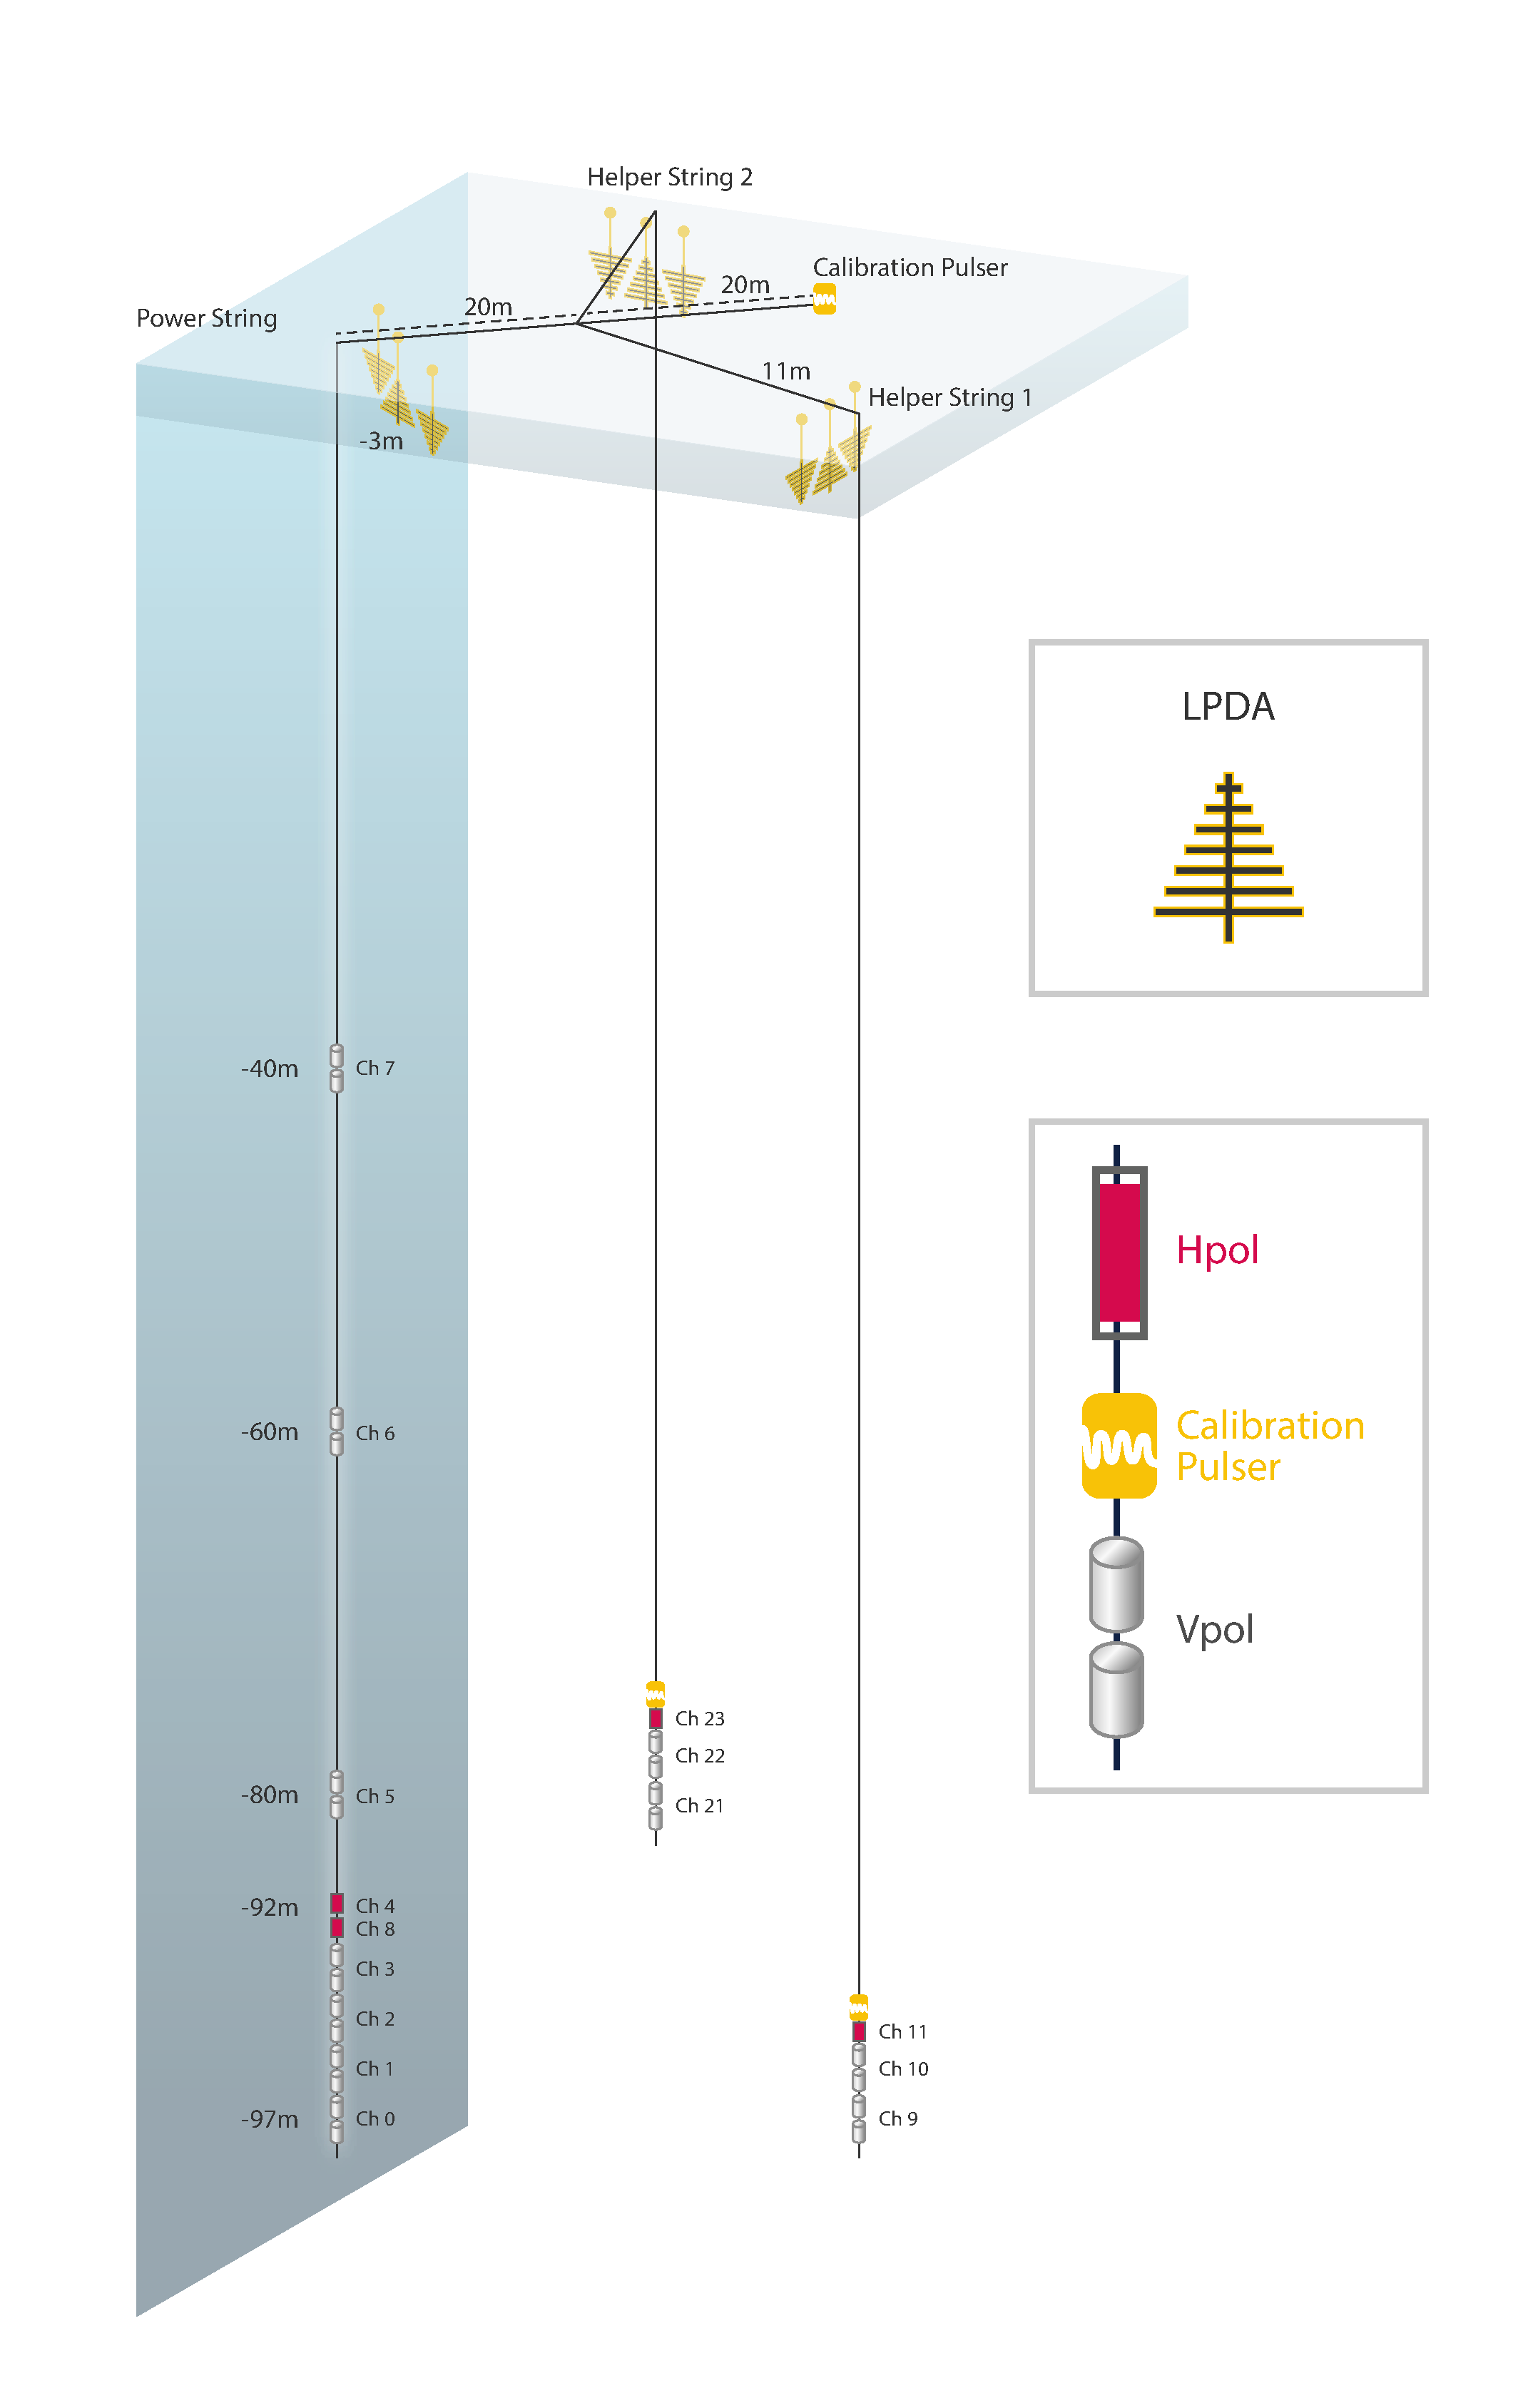
\includegraphics[height=0.9\textheight]{figures/detector.pdf}	
	\caption{illustration of the detector}
	\label{fig:detector}
\end{figure}

\begin{figure}
	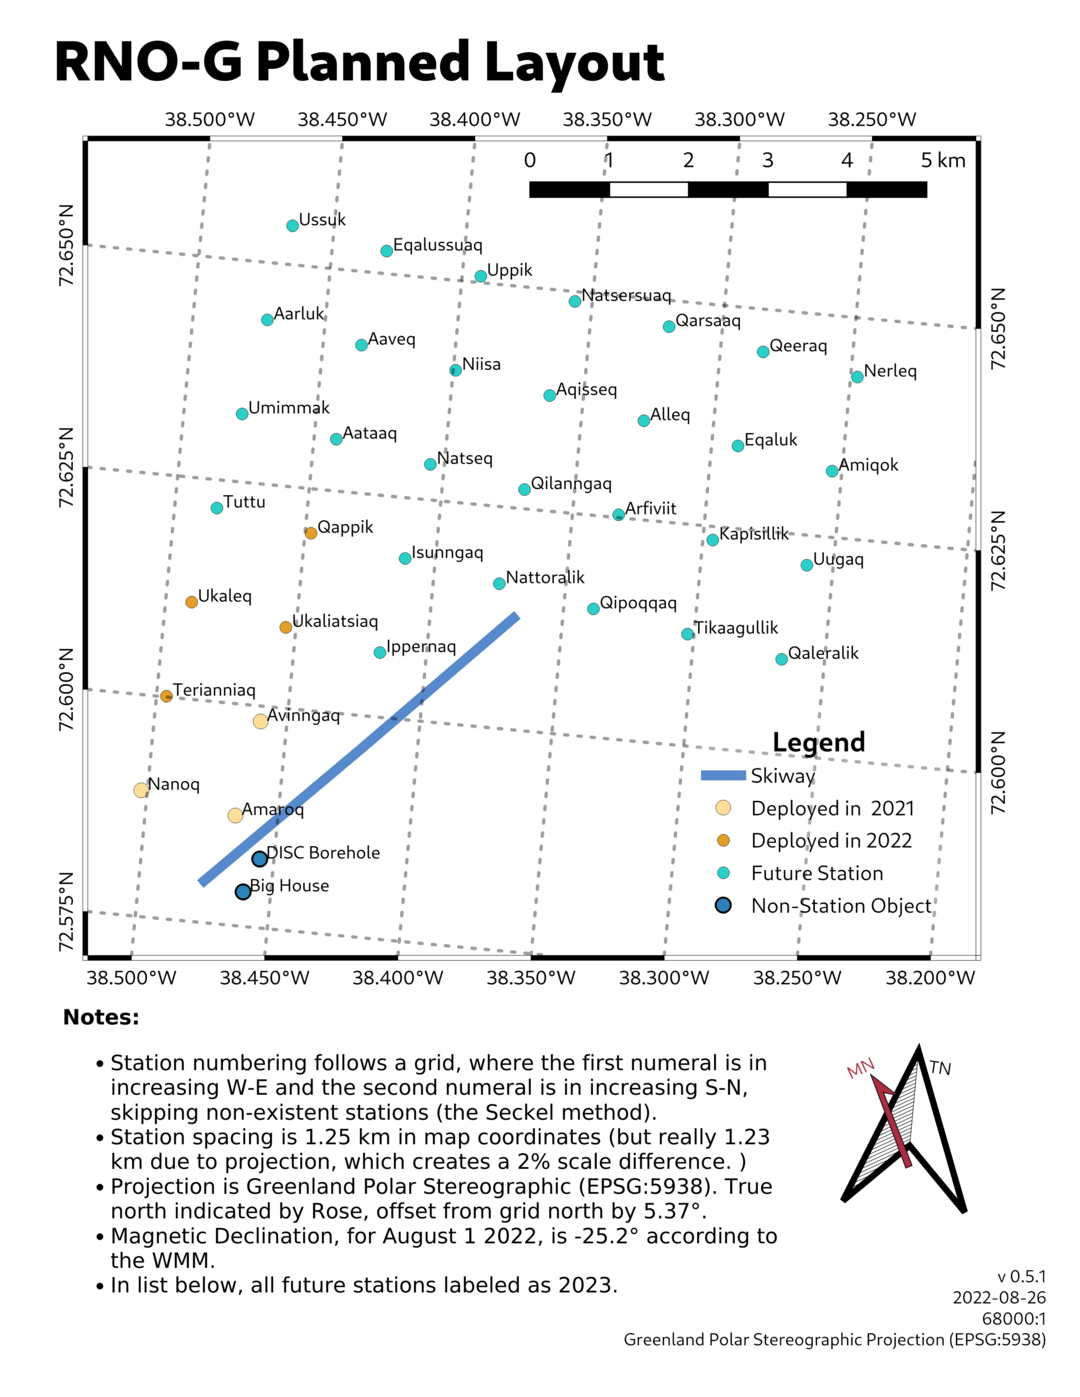
\includegraphics[width=\textwidth]{figures/station-map.png}	
	\caption{map of the station}
	\label{fig:station map}
\end{figure}

\chapter{Hybrid Ray tracer}
\label{chapter:hybrid}
%----------------------------------------------------------------------------------------
%	HYBRID RAY TRACER	
%----------------------------------------------------------------------------------------
\section{Shortcomings of the exponential ice model}
As mentioned in section \ref{section:Ice Model}, complex ice models will be
necessary moving forward as the exponential ice model fails to fit the density
curve.  The software for radio wave propagation through ice the RNO-G team chose is
radiopropa\cite{Winchen_2019}, but due to the way it works you'll have to know
the start point, the end point and the launch angle of your ray to work out the
path. This isn't difficult for the analytic model as it's exactly solvable but
for a general ice model you'll somehow have to find where to \textit{shoot} the
ray.  Work has been done on finding the launch angle in the case of complex ice
models by B. Oeyen et al. \cite{2022icrc.confE1027O}, where they created a ray
tracer which iteratively finds the solution, called the "iterative ray tracer".
The full explanation of how their algorithm works can be found in the mentioned
paper.  This is however a sub-optimal solution in python as an optimalisation
library will generally work faster, work had been done on trying to implement
such an algorithm deemed the "minimizer" but this attempt failed.  As we saw
this work the idea came to mind to combine the iterative ray tracer and the
code using the optimization libraries, to come up with the algorithm that will
be discussed in this chapter: The hybrid ray tracer, in the source code called
the "hybrid minimizer" which can be found
\href{https://github.com/arthuradriaens-code/NuRadioMC.git}{here} under the
radiopropa/hybrid\_minimizer branch.

It succeeds in more rapidly tracing the path from the event to the detector, is
more accurate and also arrives closer to the detector as the final result is
not limited by the final drawn sphere size but by a given tolerence making it
useful for plane wave reconstruction as we'll get to next chapter.

\section{How it works}
The hybrid minimizer can be seen as an extension of the iterative raytracer
\cite{2022icrc.confE1027O} as it starts out the same way: Say our source of
radiation is at position $\mathbf{X}_1$ and our detector is located at position
$\mathbf{X}_2$, we start by defining the vector $\mathbf{v} = \mathbf{X}_2 -
\mathbf{X}_1$, then we clone it as a new vector u and set u's z coordinate to
0, making it a normal vector of a plane parallel to the z direction. we now
wish to know where we'd actually be able to find possible paths, looking at
figure \ref{fig:PathIllu} we see that no solutions below the direct path are
possible as there would need to be upwards reflection, so we convert our vector
$\mathbf{v}$ representing the path from the source to the detector to spherical
coordinates, giving us a polar angle (zenith angle) "theta-direct". With this
we know that at the source the ray should propagate with an initial zenith
angle within the angle interval 0° to theta-direct° $:= \Omega$.

Next we need to define our "observers", if you shoot a ray with the radiopropa
module from a certain point at a certain angle the ray path will get simulated
until it interacts with this "observer".  Ideally we would like to a priori
know where to shoot our ray and have the detector be an infinitesimally small
observer in our simulation, but as we'll be working with general ice models
this can't be done.

The algorithm of finding the possible paths is then as follows: We define a
spherical observer at the location of the detector, with a radius of fair size.
We place an observer plane directly behind the detector (with normal vector
$\mathbf{u}$, no rays can propagate back after crossing) and an observer above
the surface (as no rays could make it back after escaping the ice) our full
setup is then what's illustrated in the figure below

Here the red cross is the radio source, the blue horizontal line is the ice-air
boundary surface, the blue dot to the right is the detector and the green
$\Omega$ indicates the range over which solutions to the problem are possible.

We start off by just iteratively guessing: given a certain angle stepsize
$\Delta \theta$ shoot rays at the angles $\{0,\Delta \theta, 2\Delta
\theta,...,\Omega\}$ And see which ones get detected at the sphere around the
detector, this process is illustrated in a modified version of B. Oeyen et al.
their figure below\\
\begin{figure}[h!]
  \centering
  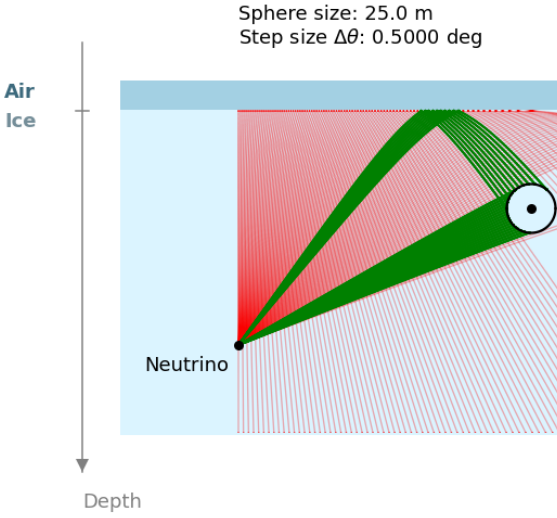
\includegraphics[width=0.5\textwidth]{begin_explanation.png}
\end{figure}\\
if there are 2 distinct launch regions, it will start the so called "minimization", using scipy's module 
optimize.minimize. First we get rid of the spherical observer and place the vertical observer exactly at
the detector, now
to be able to use the minimize module we'll need a function to minimze, for this reason we define the function 
\textit{delta\_z} as, given a certain launch angle, returning the distance from the point where it lands on the
plane to the detector as illustrated below
\begin{figure}[h!]
  \centering
  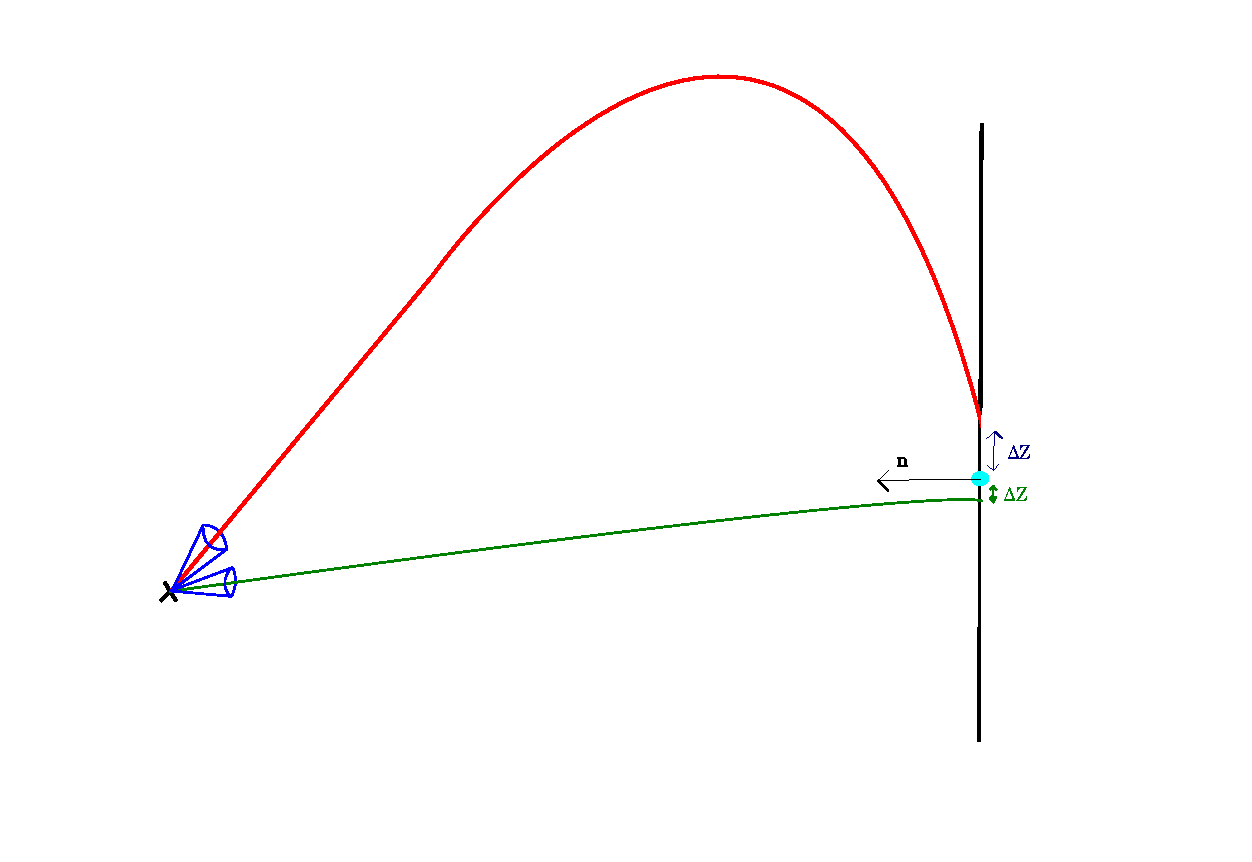
\includegraphics[width=0.5\textwidth]{PrincipleHybridIllu.pdf}
\end{figure}\\
The function we'll minimize is then detla\_z\_squared which is just the square of delta\_z as we wish it to be
as close as possible to 0, it gets minimized within the angle boundaries found from the previous step.
With this our algorithm is done, it does have a fail-safe as well for if the first step, finding the launch
regions, doesn't work namely it reverts back to being the iterative ray tracer.
\section{Performance Optimalisation}
To test the hybrid minimizer the numpy random module was used to generate
random coördinates, the considered square (as there is only a z component to
the ice model the 3D problem is cilindrically symmetric and thus essentially
only a 2D problem) is x:0.1km,4km and z:-0.1km,-3km.\footnote{This start at
100m depth was to get around issues concerning events that won't even trigger
in a full simulation} Every test point shown in the following subsections
consists of at least 500 random initial positions.  As the speed of the
algorithm is computer dependent the algorithm's speed is always plotted
relative to the iterative ray tracer's speed, simulated with the same
coordinates at the same time.
\subsection{Length of the normal vector}
\begin{figure}[h!]
	\centering
	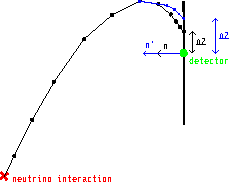
\includegraphics[width=0.7\textwidth]{figures/PrincipleNormIllu.pdf}
	\caption{how normal vector size influences the stepsize}
	\label{fig:normexpl}
\end{figure}
As visually explained in figure \ref{fig:normexpl}, the size of the normal vector seems to
influence how big the ray tracer's step size is taken close to the detector. This
thus influences the convergence and time taken. The results of varying this are shown
in figures \ref{fig:norminfl} and \ref{fig:norminfl2}.
Looking at these figures the first optimization conclusion is as expected: 
take the normal vector length to be 1 meter.
\subsection{ztol}
We'll now change the tolerence on the vertical distance away from the detector which is deemed
accepted i.e in figure \ref{fig:normexpl} if $\Delta z$ is below this threshold it's accepted.
The results are shown in figures \ref{fig:ztolinfl} and \ref{fig:ztolinfl2}.
From which we can conclude the second optimization conclusion: take ztol to be 0.05 m.
\subsection{Sphere Size \& Step Size}
The initial rays are sent out in steps of a certain angle and with a sphere
around the detector of a certain size. As this initial search for launch angle
regions is the slowest step in the hybrid ray tracer it's imperative to
optimize this. The procedure was: change the sphere size and loop over various
step sizes, recording the speed. The results are shown in figure \ref{fig:SphereStepInfl} 
the lower on the chart the better, zooming in onto the lowest point as is shown in a combined
plot on figure \ref{fig:SphereStepFinal}, we see that an optimum seems to be around a spheresize
of 45m and a stepsize of 0.7°.

\begin{figure*}
	\centering
\begin{minipage}{0.49\textwidth}
	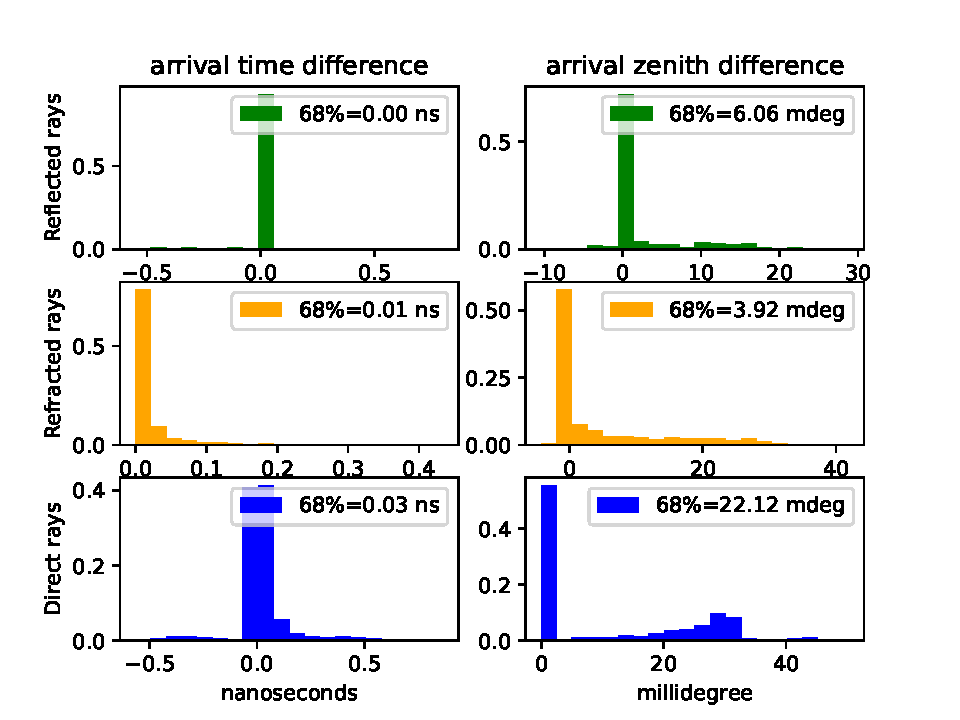
\includegraphics[width=1.1\textwidth]{figures/hybrid_comparison_N_1000.pdf}
	\caption{Hybrid}
	\label{fig:acchyb}
\end{minipage}
\begin{minipage}{0.49\textwidth}
	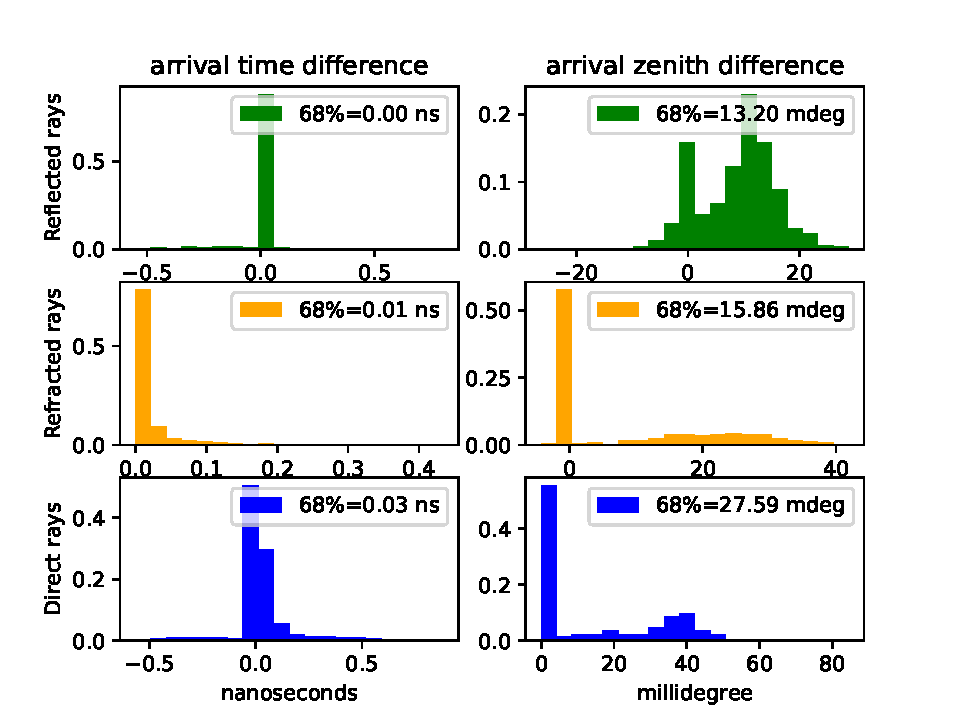
\includegraphics[width=1.1\textwidth]{figures/iterative_comparison_N_1000.pdf}
	\caption{Iterative}
	\label{fig:accit}
\end{minipage}
\end{figure*}

\begin{figure}
	\centering
	\begin{minipage}{\textwidth}
		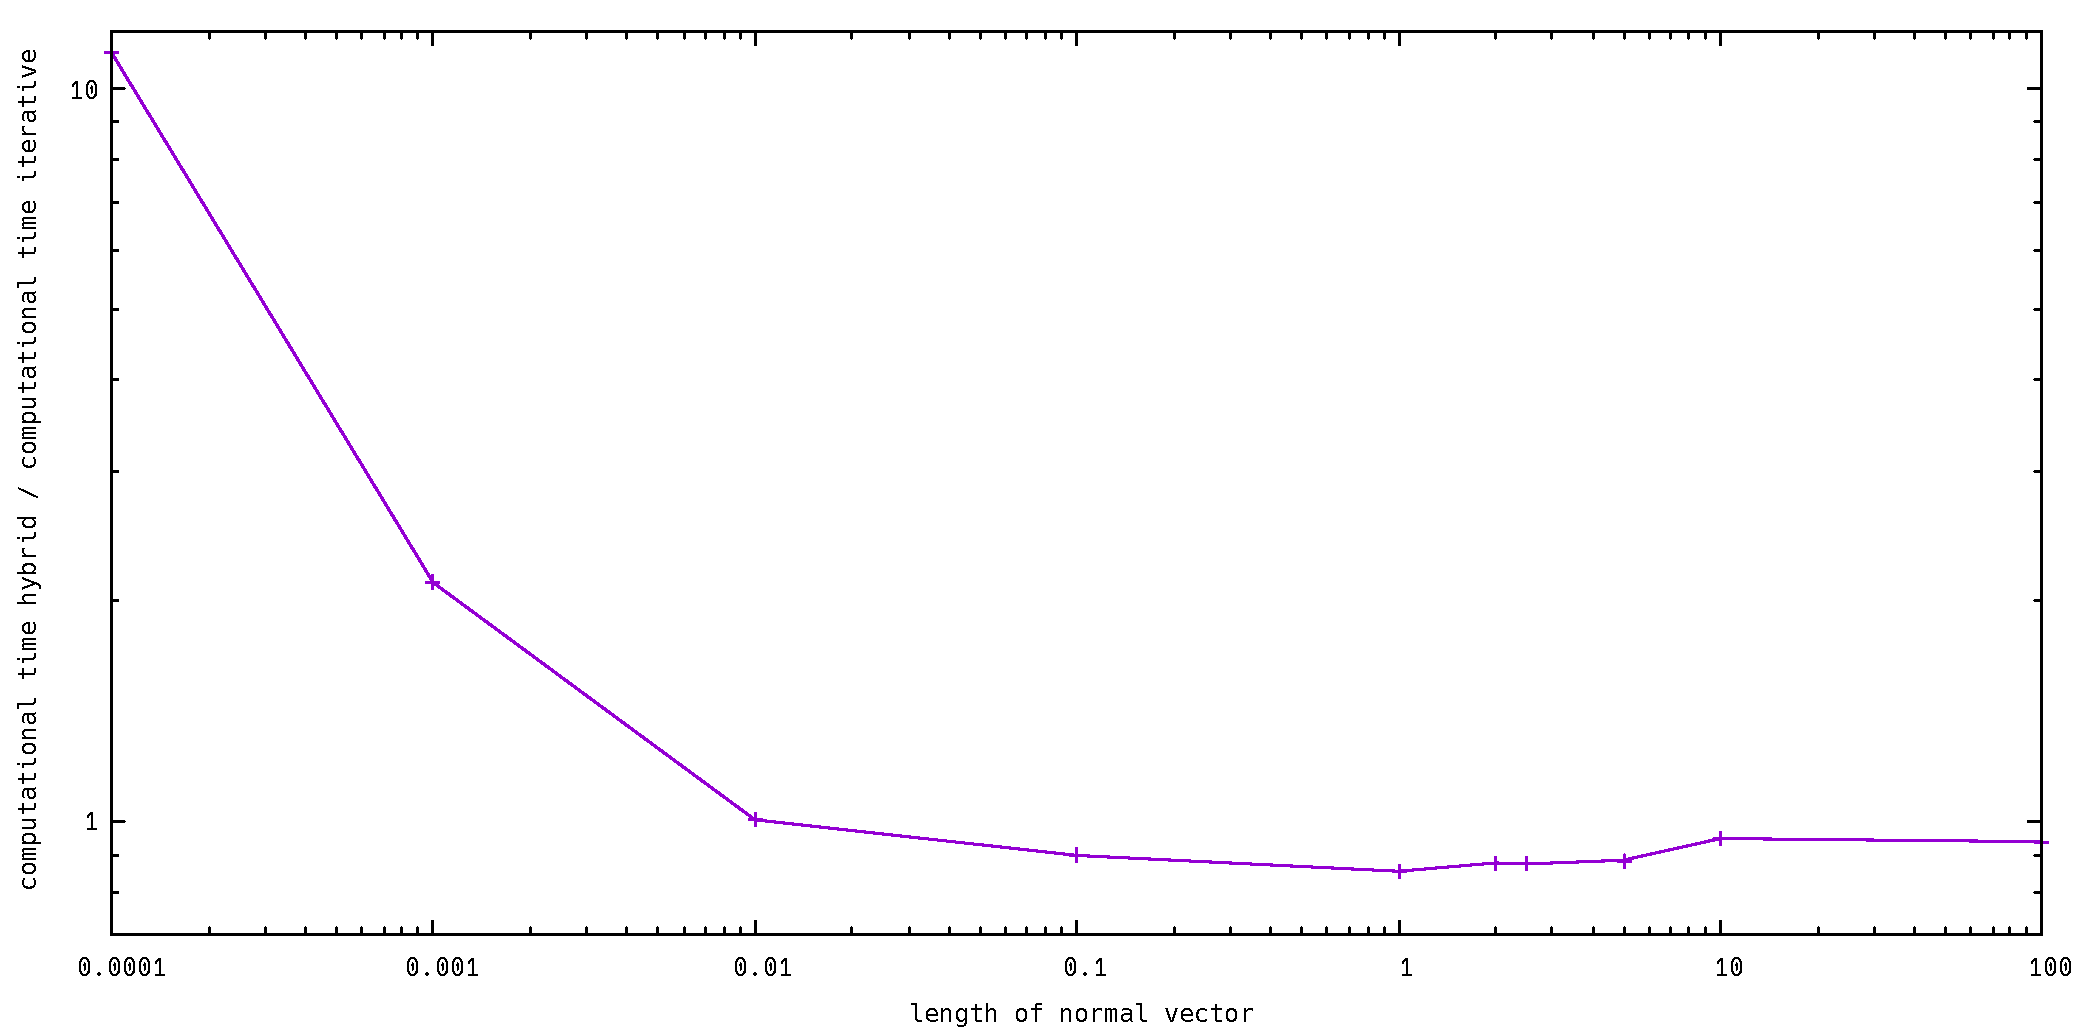
\includegraphics[width=0.8\textwidth]{figures/NormVsTime.pdf}
	\end{minipage}
	\begin{minipage}{\textwidth}
		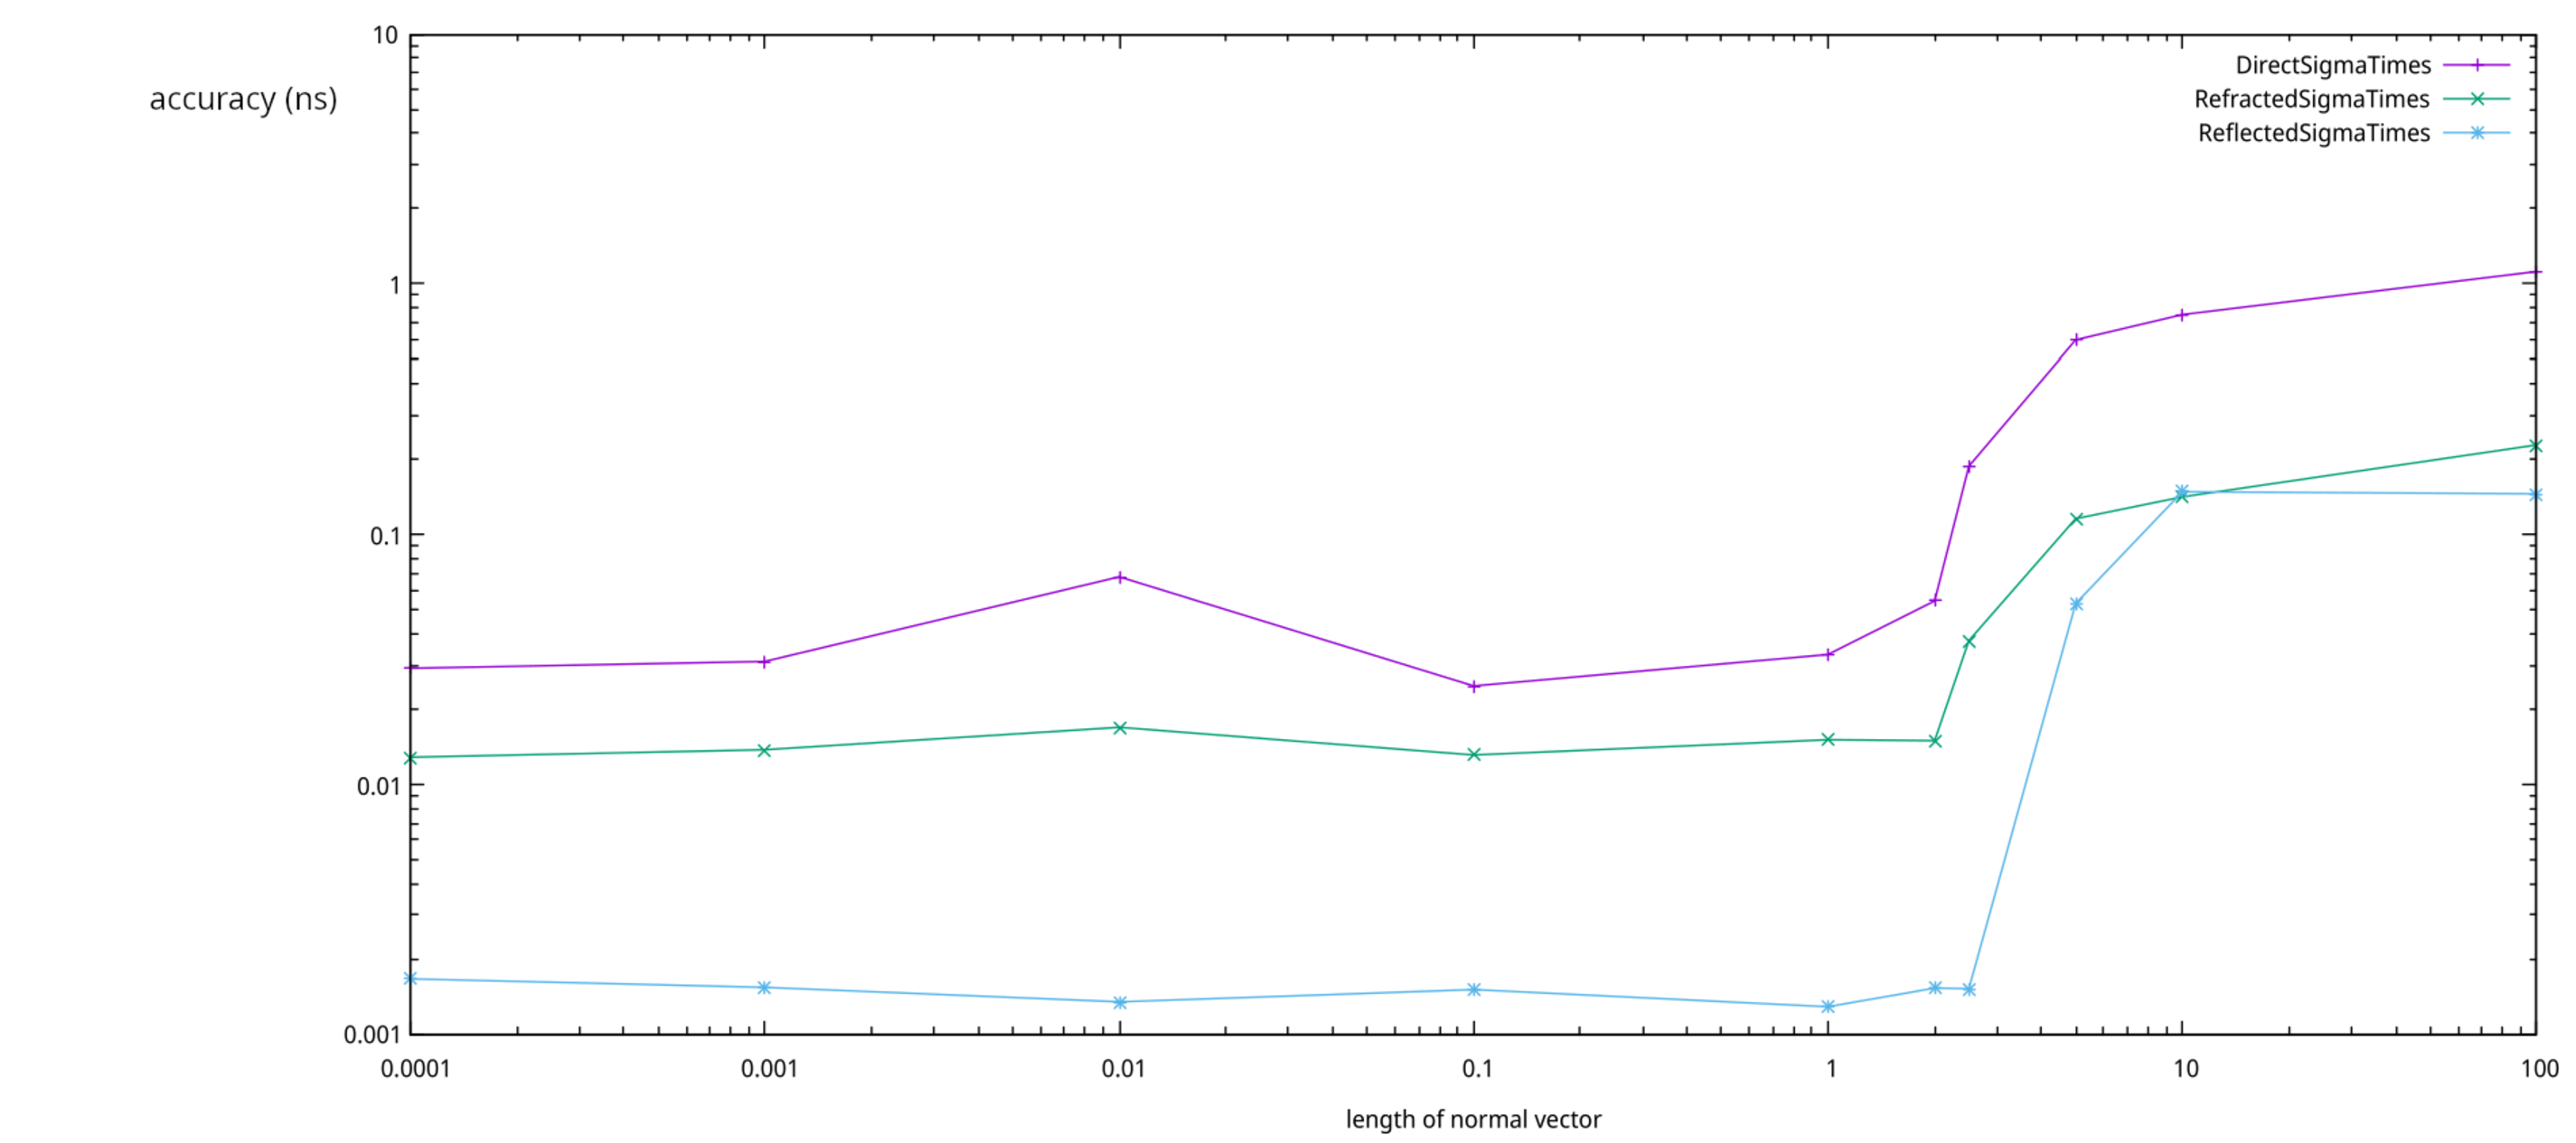
\includegraphics[width=0.8\textwidth]{figures/NormVsSigmaTime.pdf}
	\end{minipage}
\caption{influence of the length of the normal vector}
\label{fig:norminfl}
\end{figure}
\begin{figure}
	\centering
	\begin{minipage}{\textwidth}
		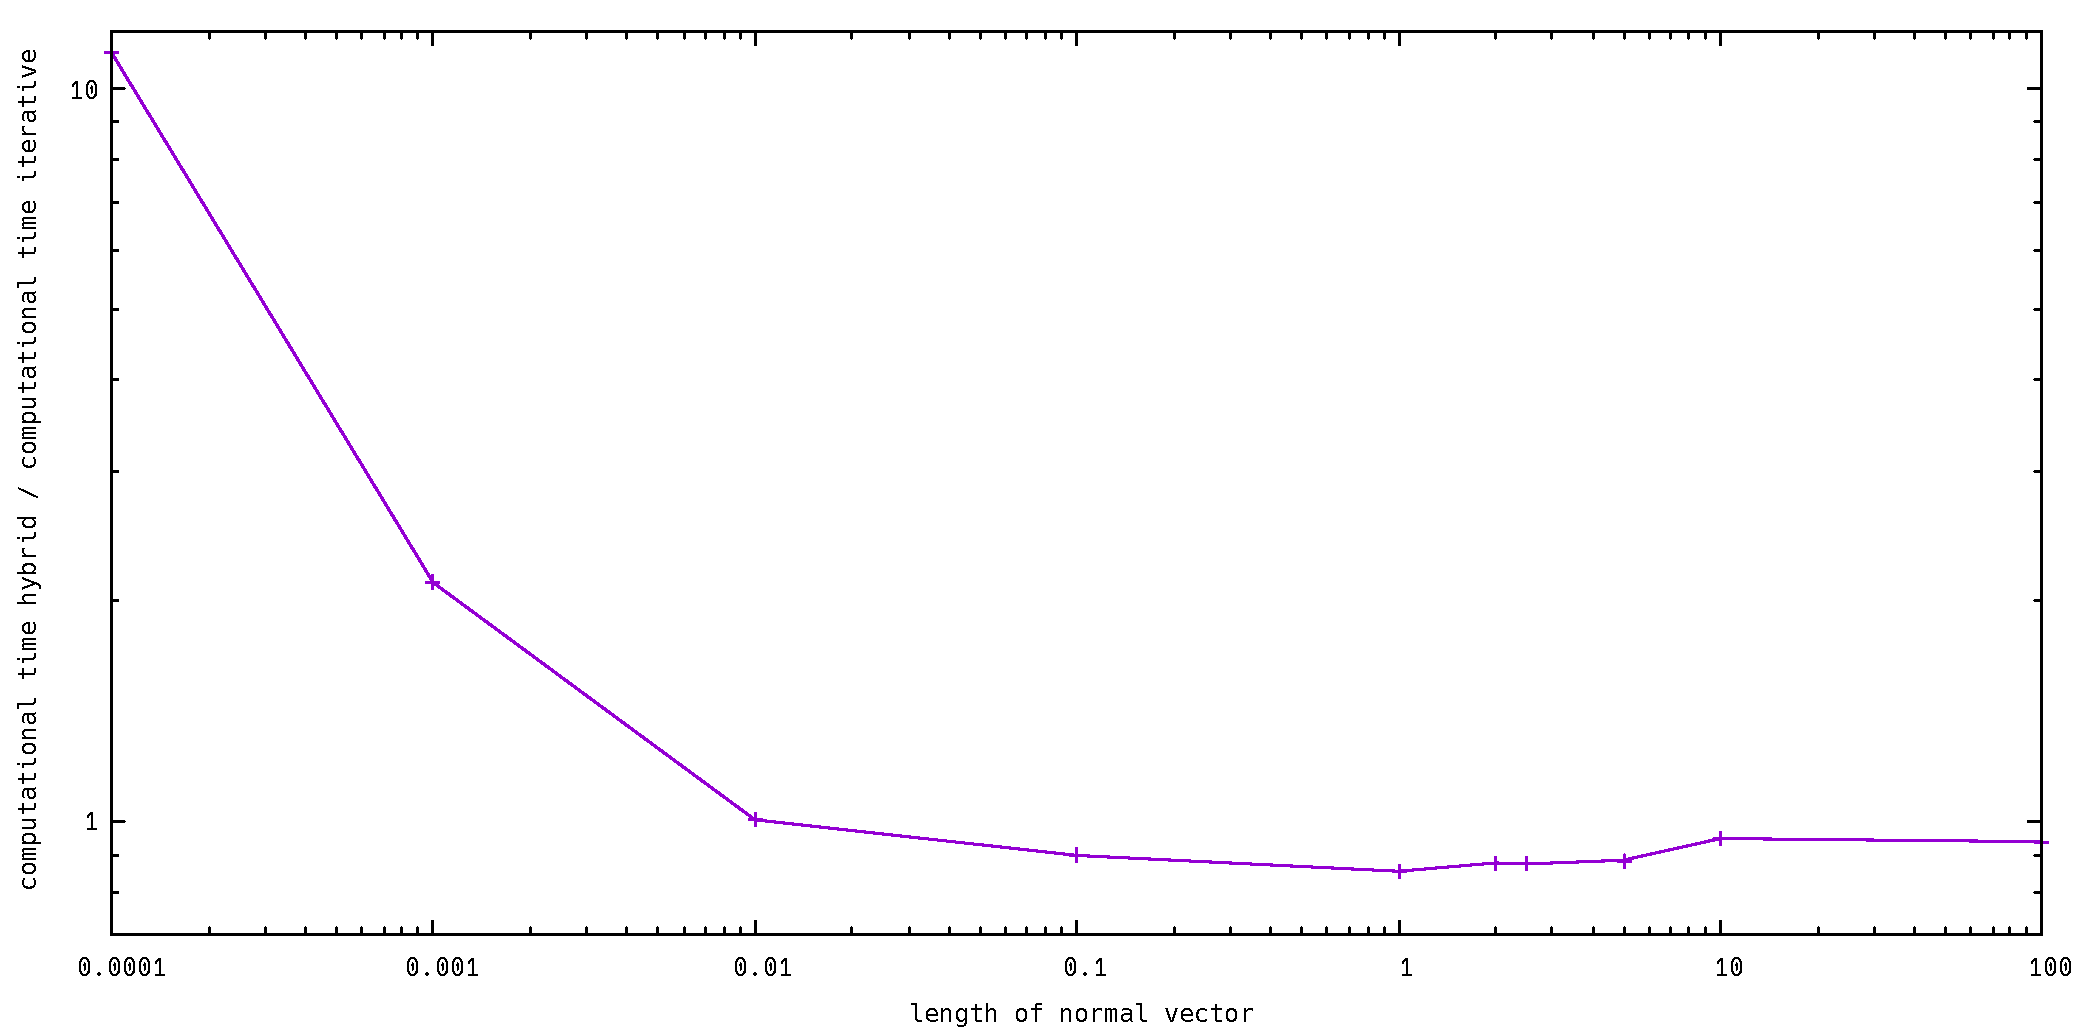
\includegraphics[width=0.8\textwidth]{figures/NormVsTime.pdf}
	\end{minipage}
	\begin{minipage}{\textwidth}
		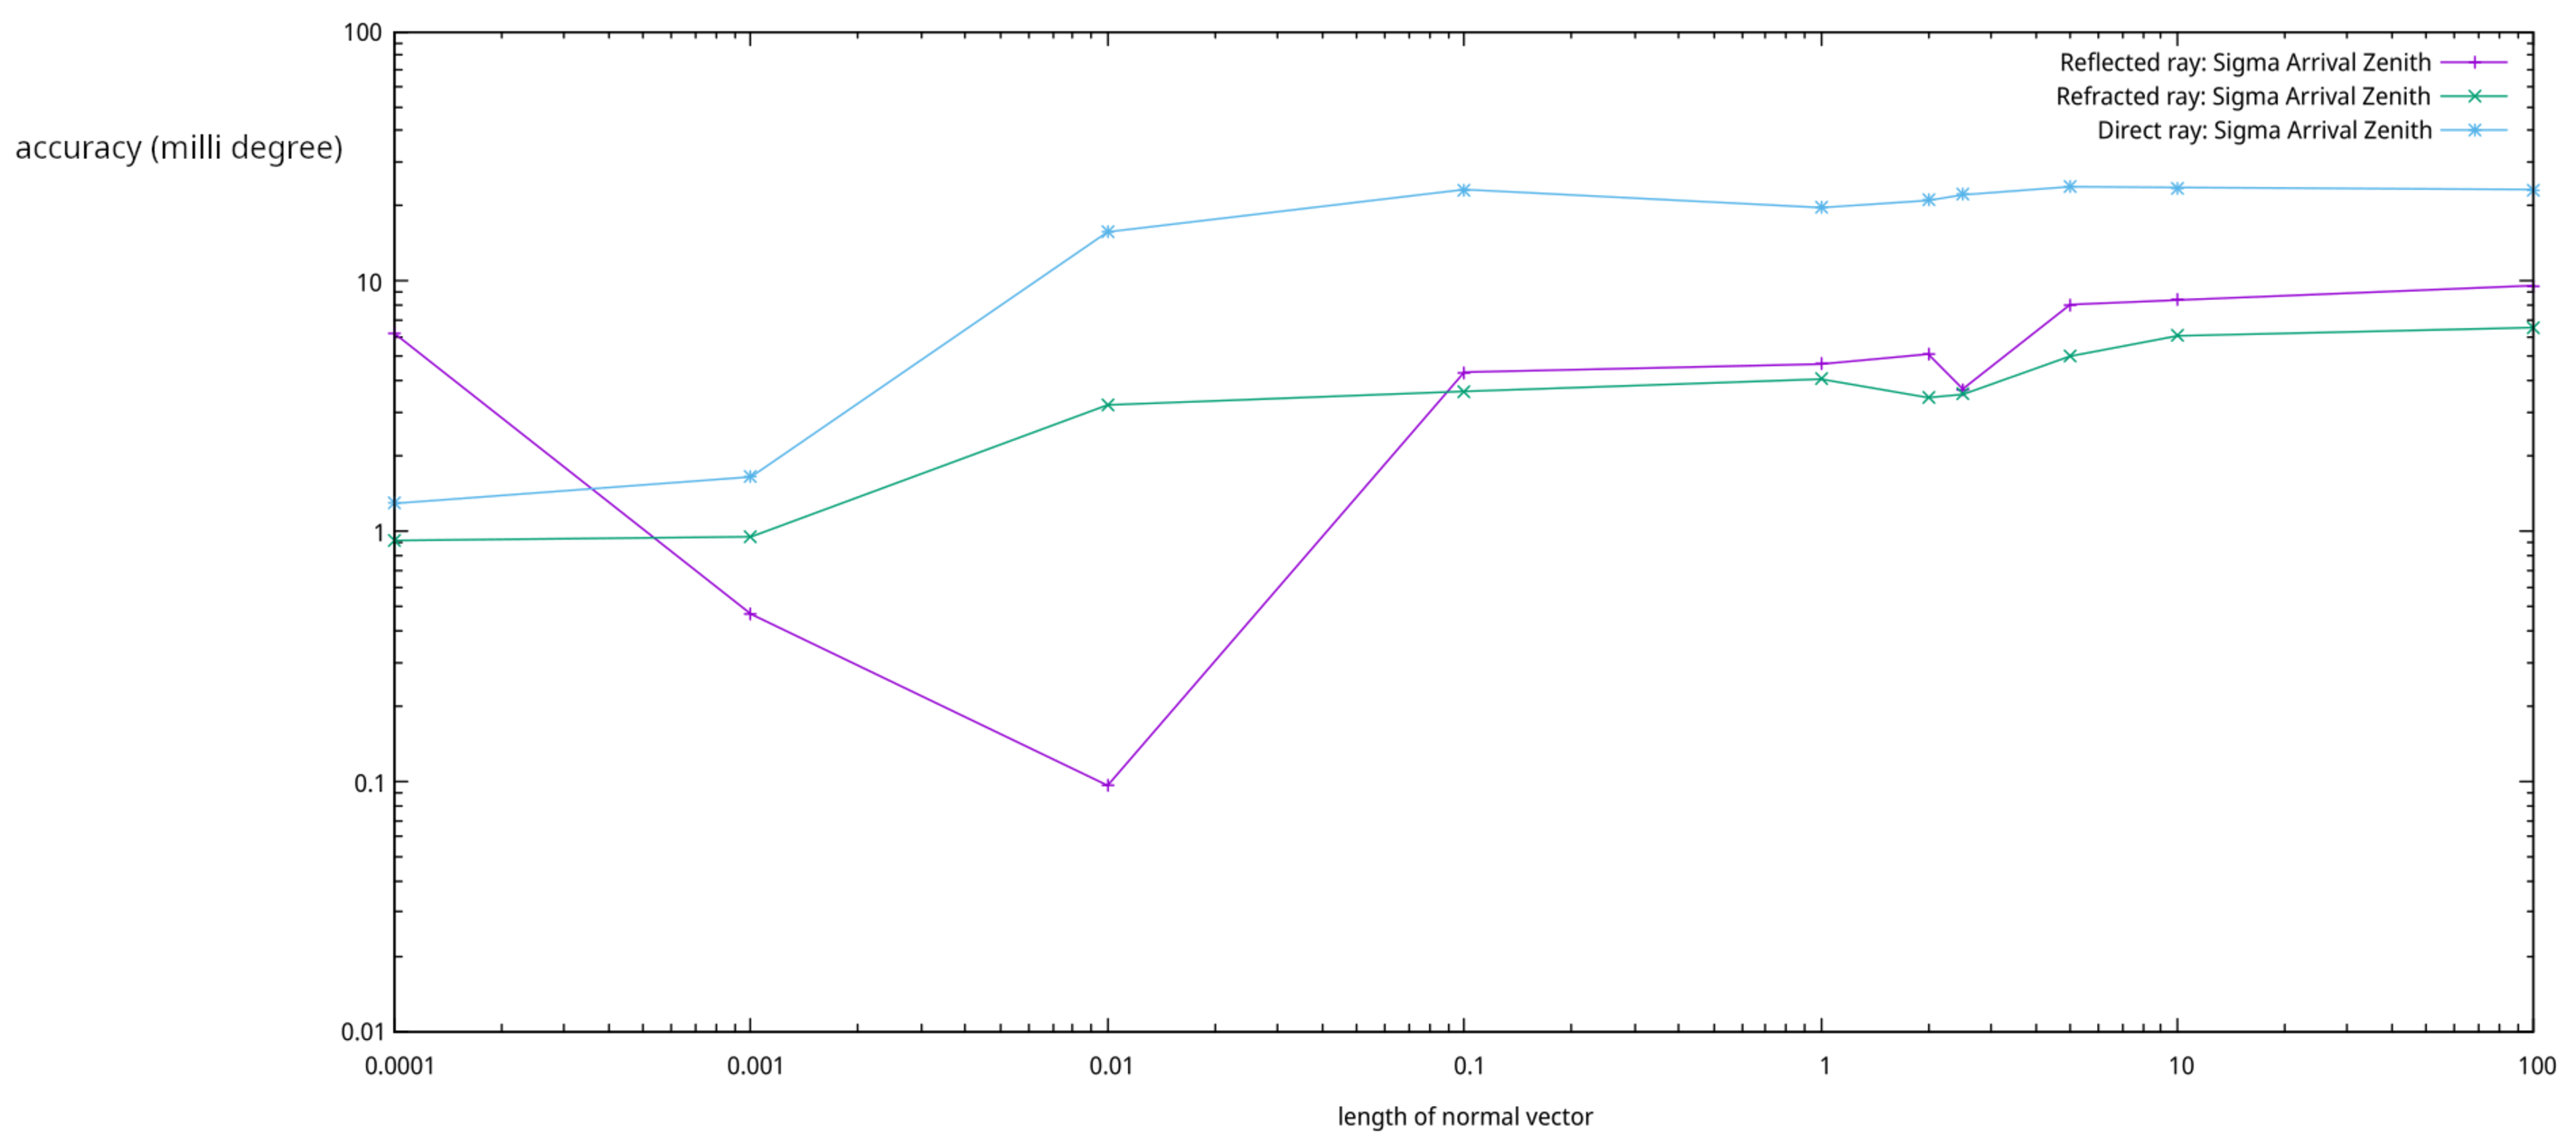
\includegraphics[width=0.8\textwidth]{figures/NormVsSigmaAZ.pdf}
	\end{minipage}
\caption{influence of the length of the normal vector}
\label{fig:norminfl2}
\end{figure}

\begin{figure}
	\centering
	\begin{minipage}{\textwidth}
		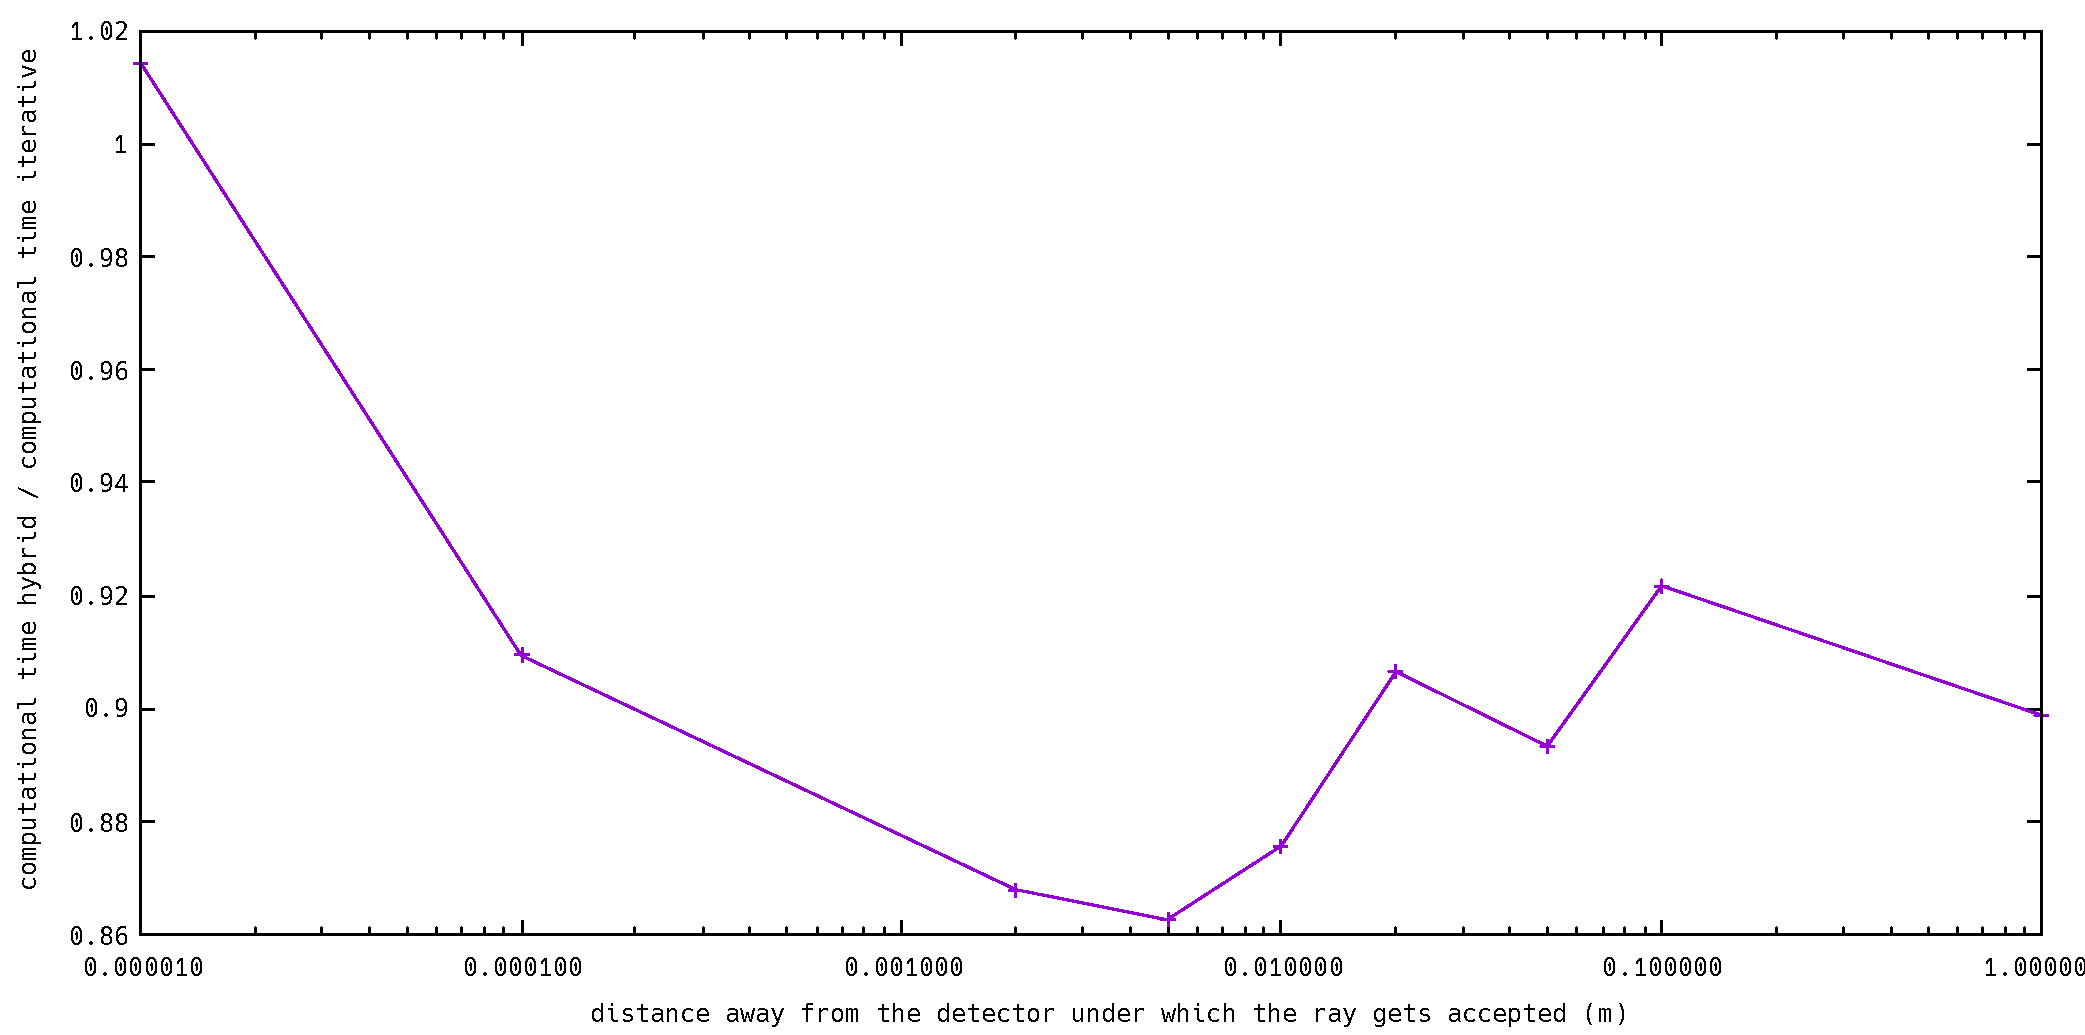
\includegraphics[width=0.8\textwidth]{figures/ZtolVsTime2.pdf}
	\end{minipage}
	\begin{minipage}{\textwidth}
		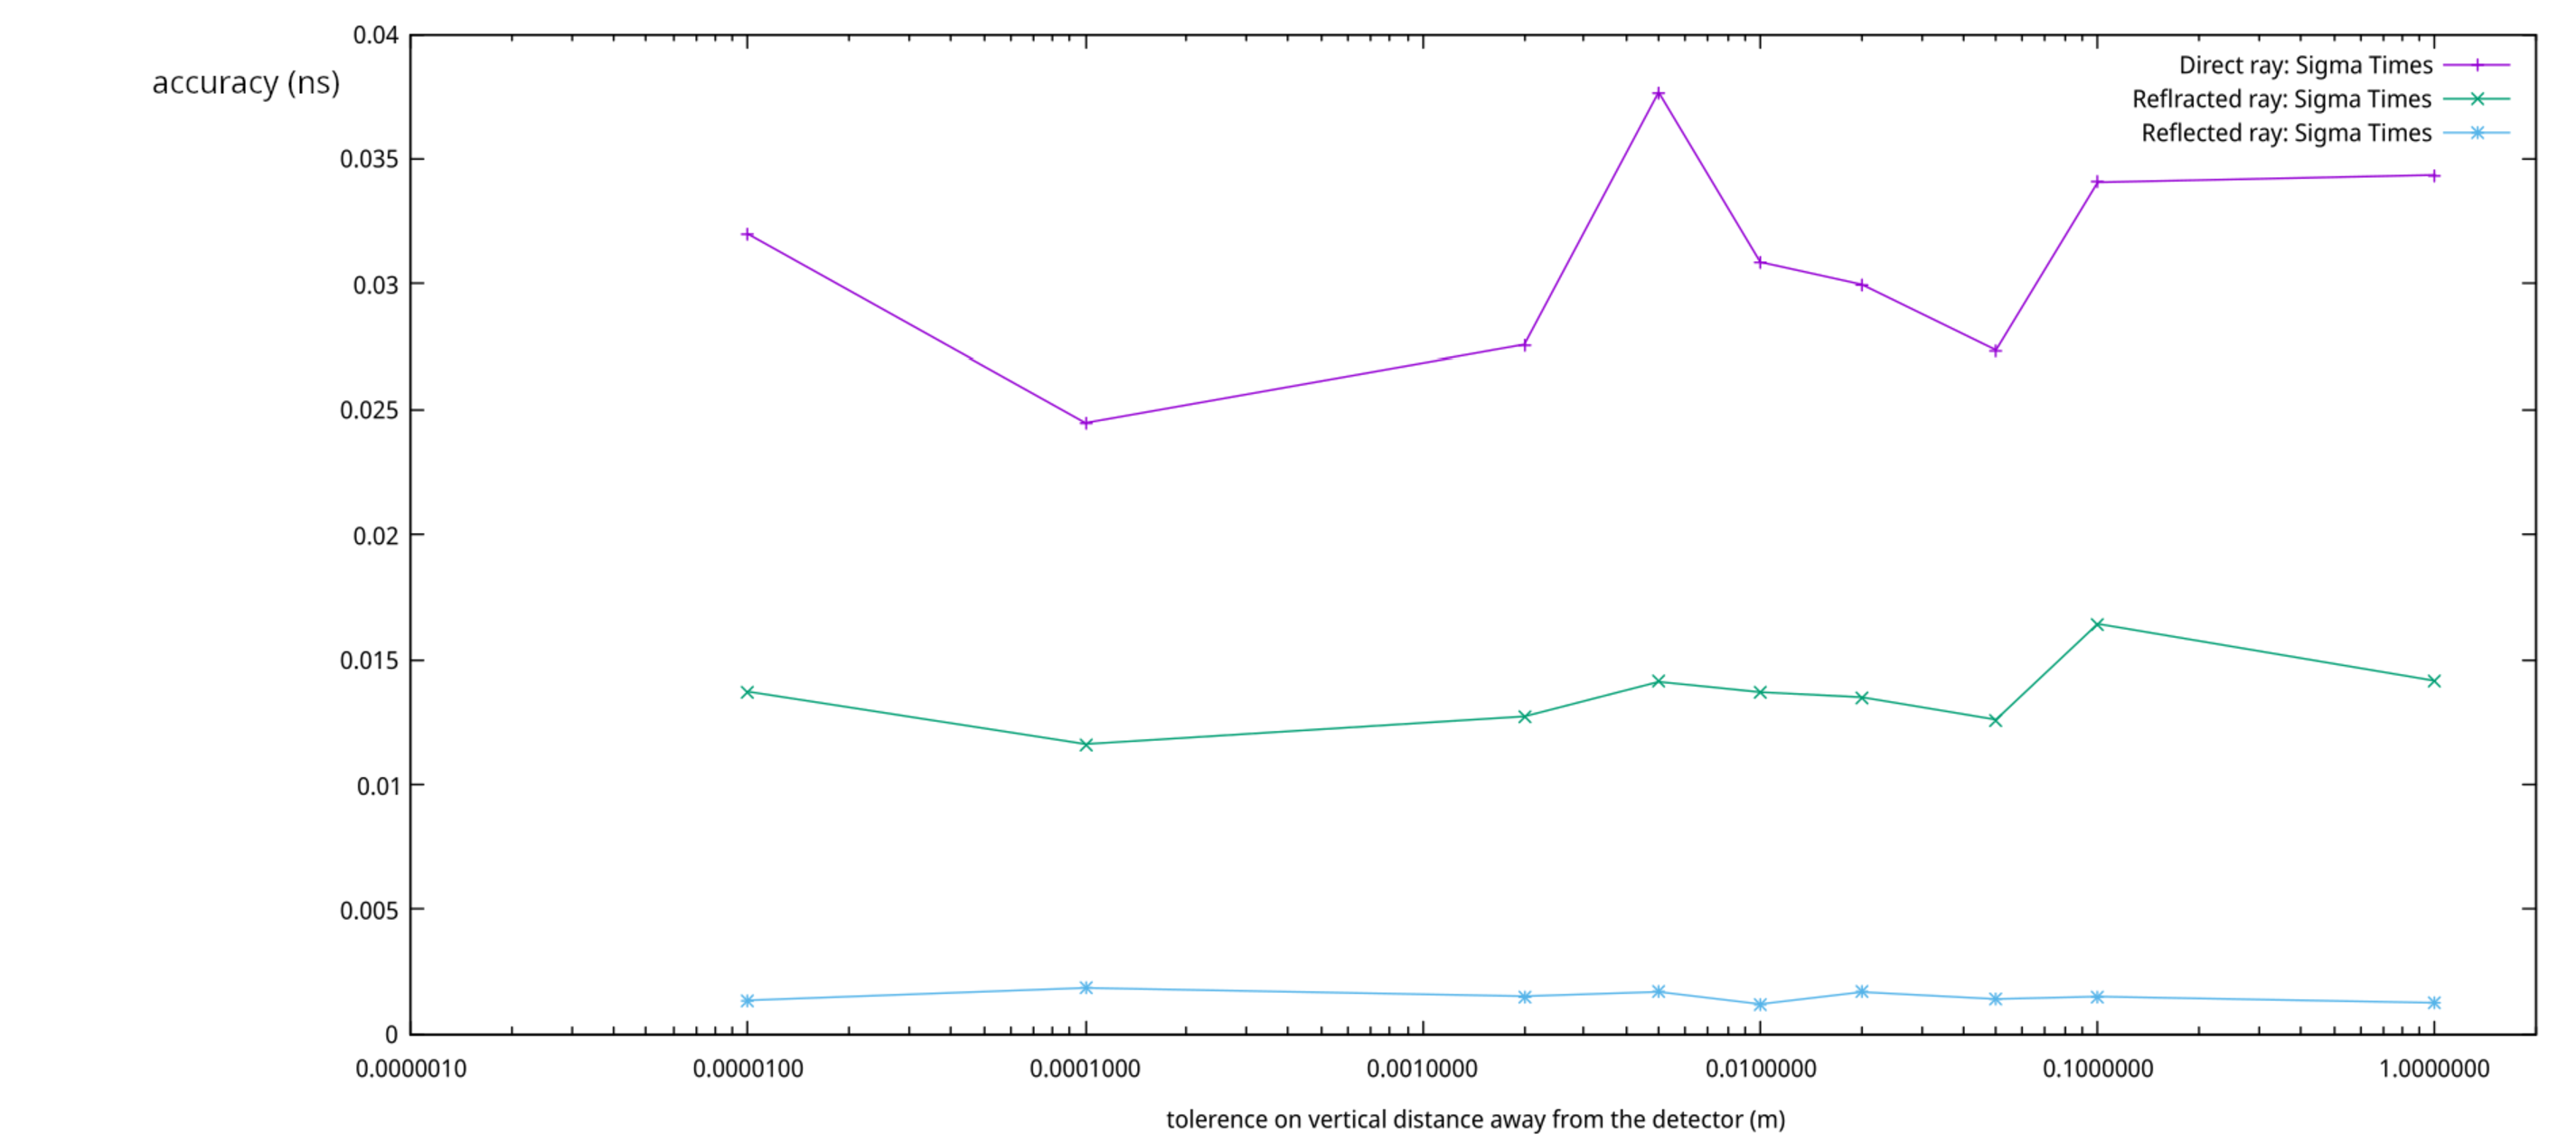
\includegraphics[width=0.8\textwidth]{figures/ZtolVsSigmaTime.pdf}
	\end{minipage}
\caption{influence of the tolerence on vertical distance}
\label{fig:ztolinfl}
\end{figure}

\begin{figure}
	\centering
	\begin{minipage}{\textwidth}
		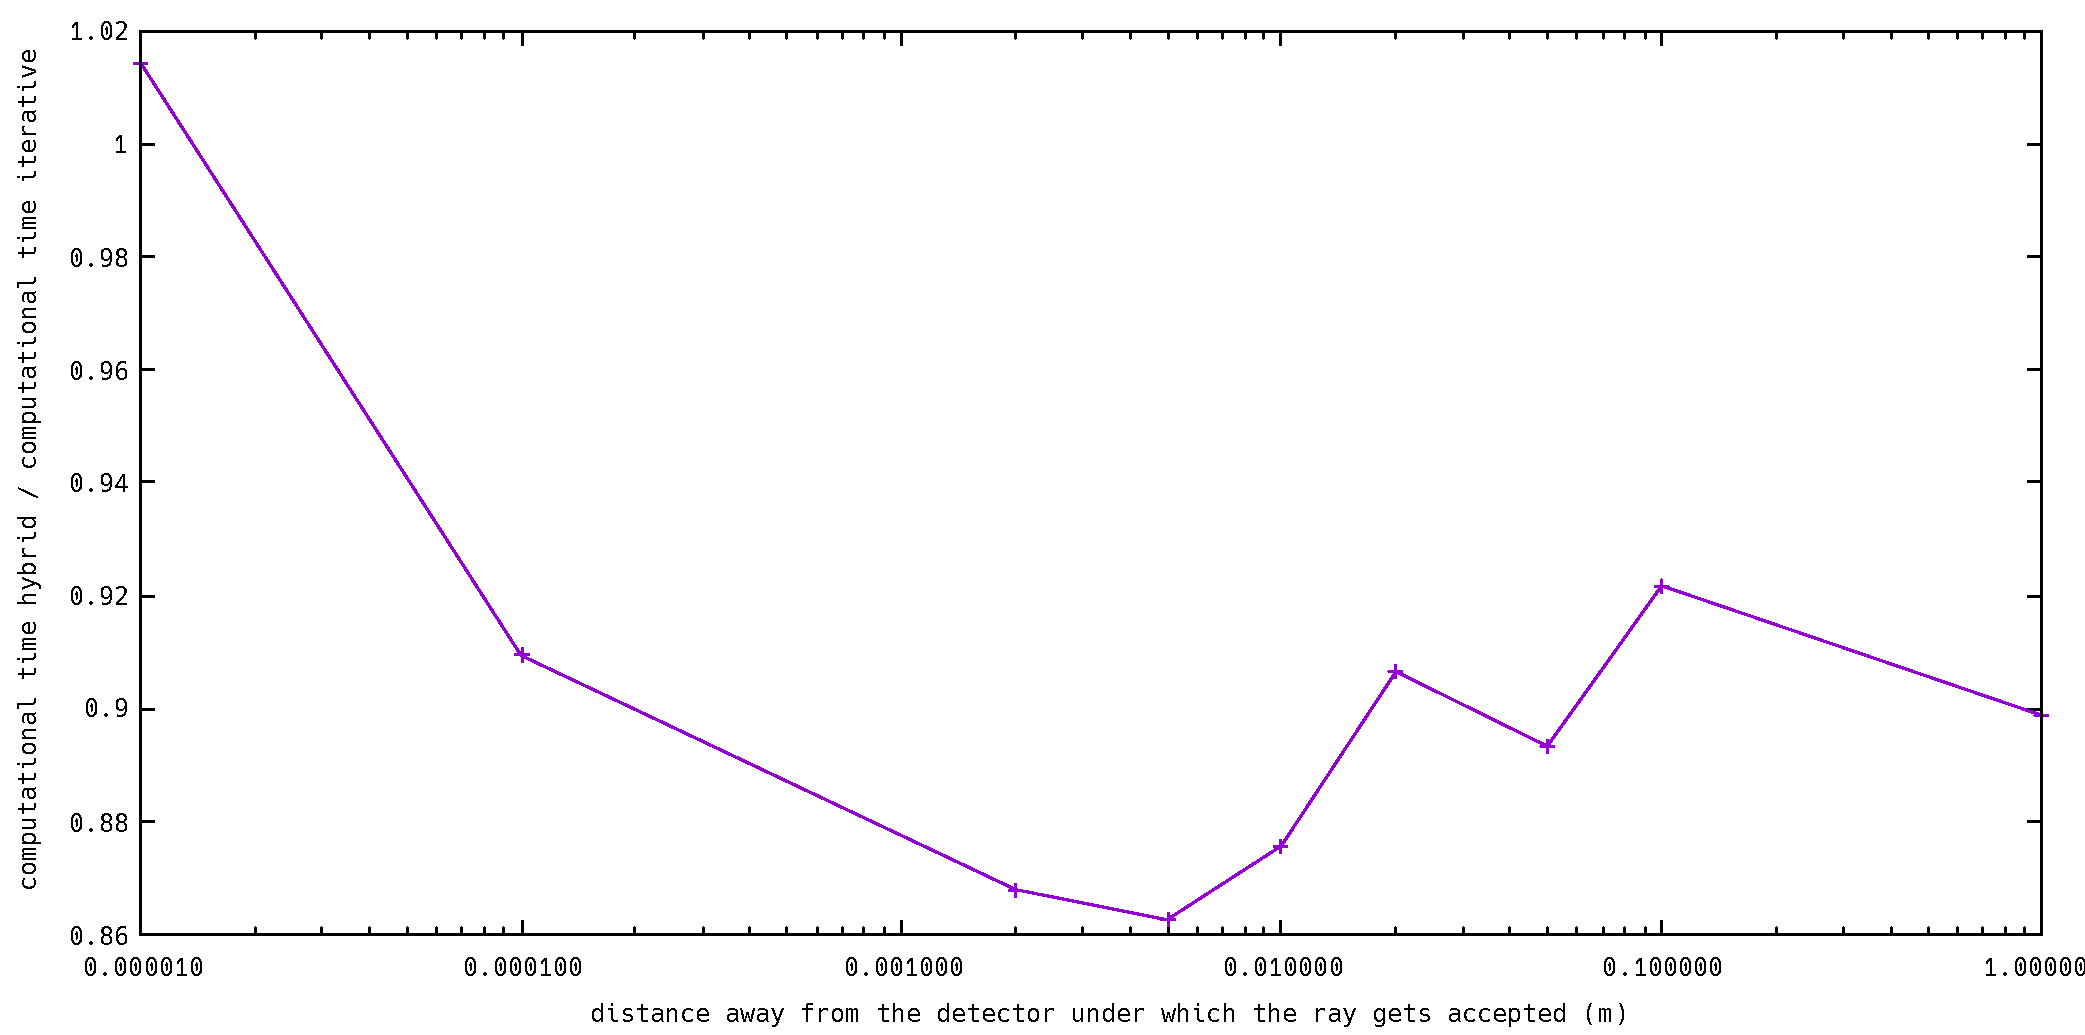
\includegraphics[width=0.8\textwidth]{figures/ZtolVsTime2.pdf}
	\end{minipage}
	\begin{minipage}{\textwidth}
		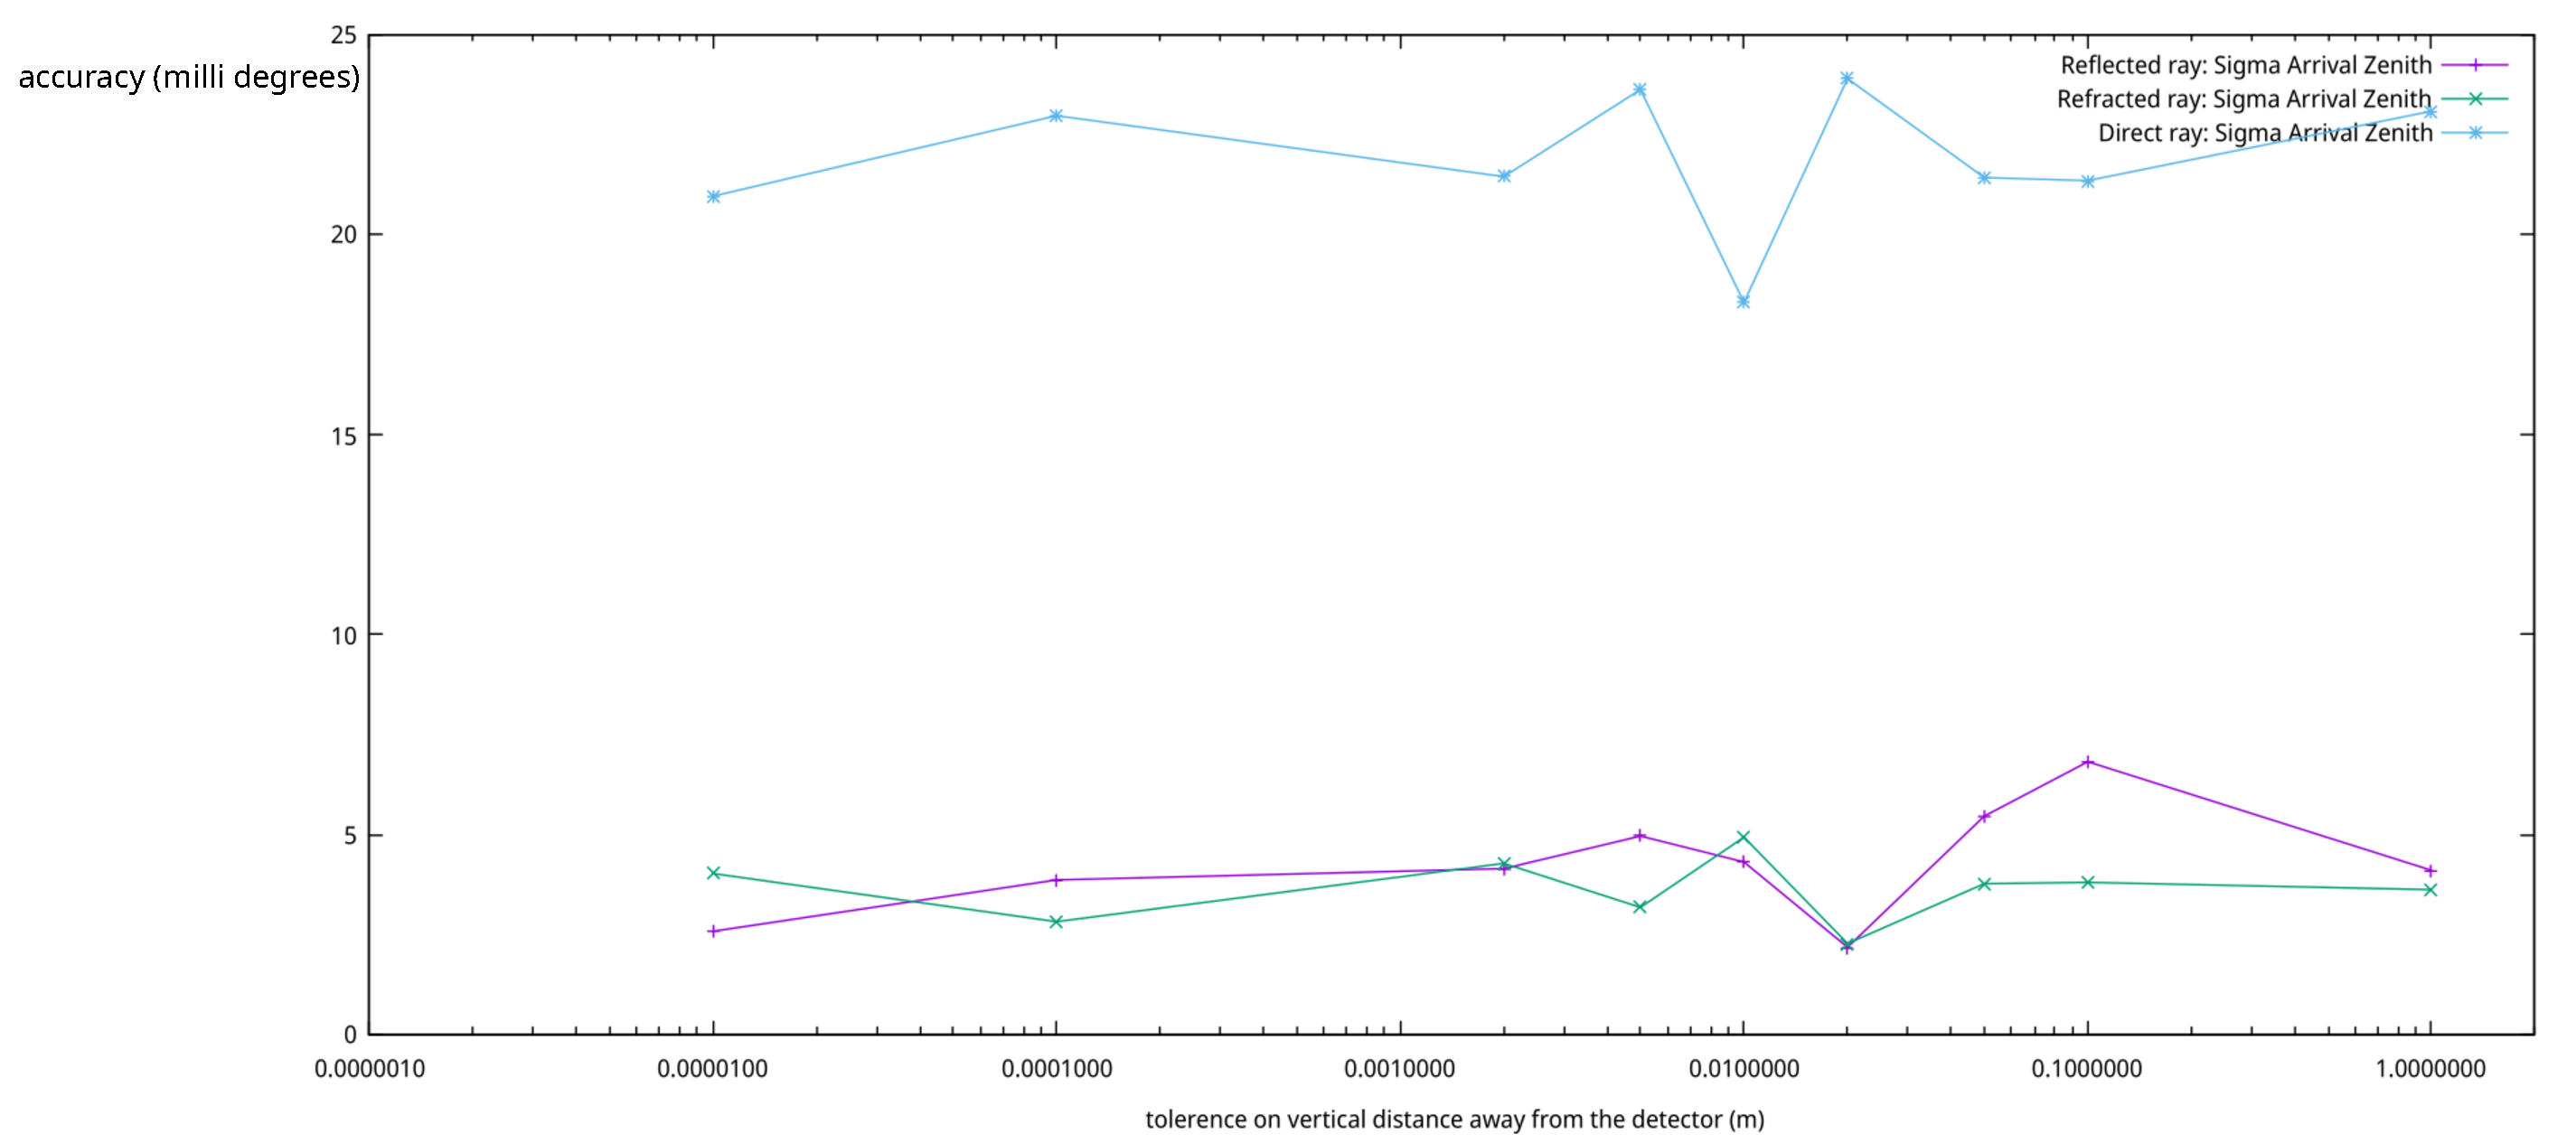
\includegraphics[width=0.8\textwidth]{figures/ZtolVsSigmaAZ.pdf}
	\end{minipage}
\caption{influence of the tolerence on vertical distance}
\label{fig:ztolinfl2}
\end{figure}

\begin{figure}
	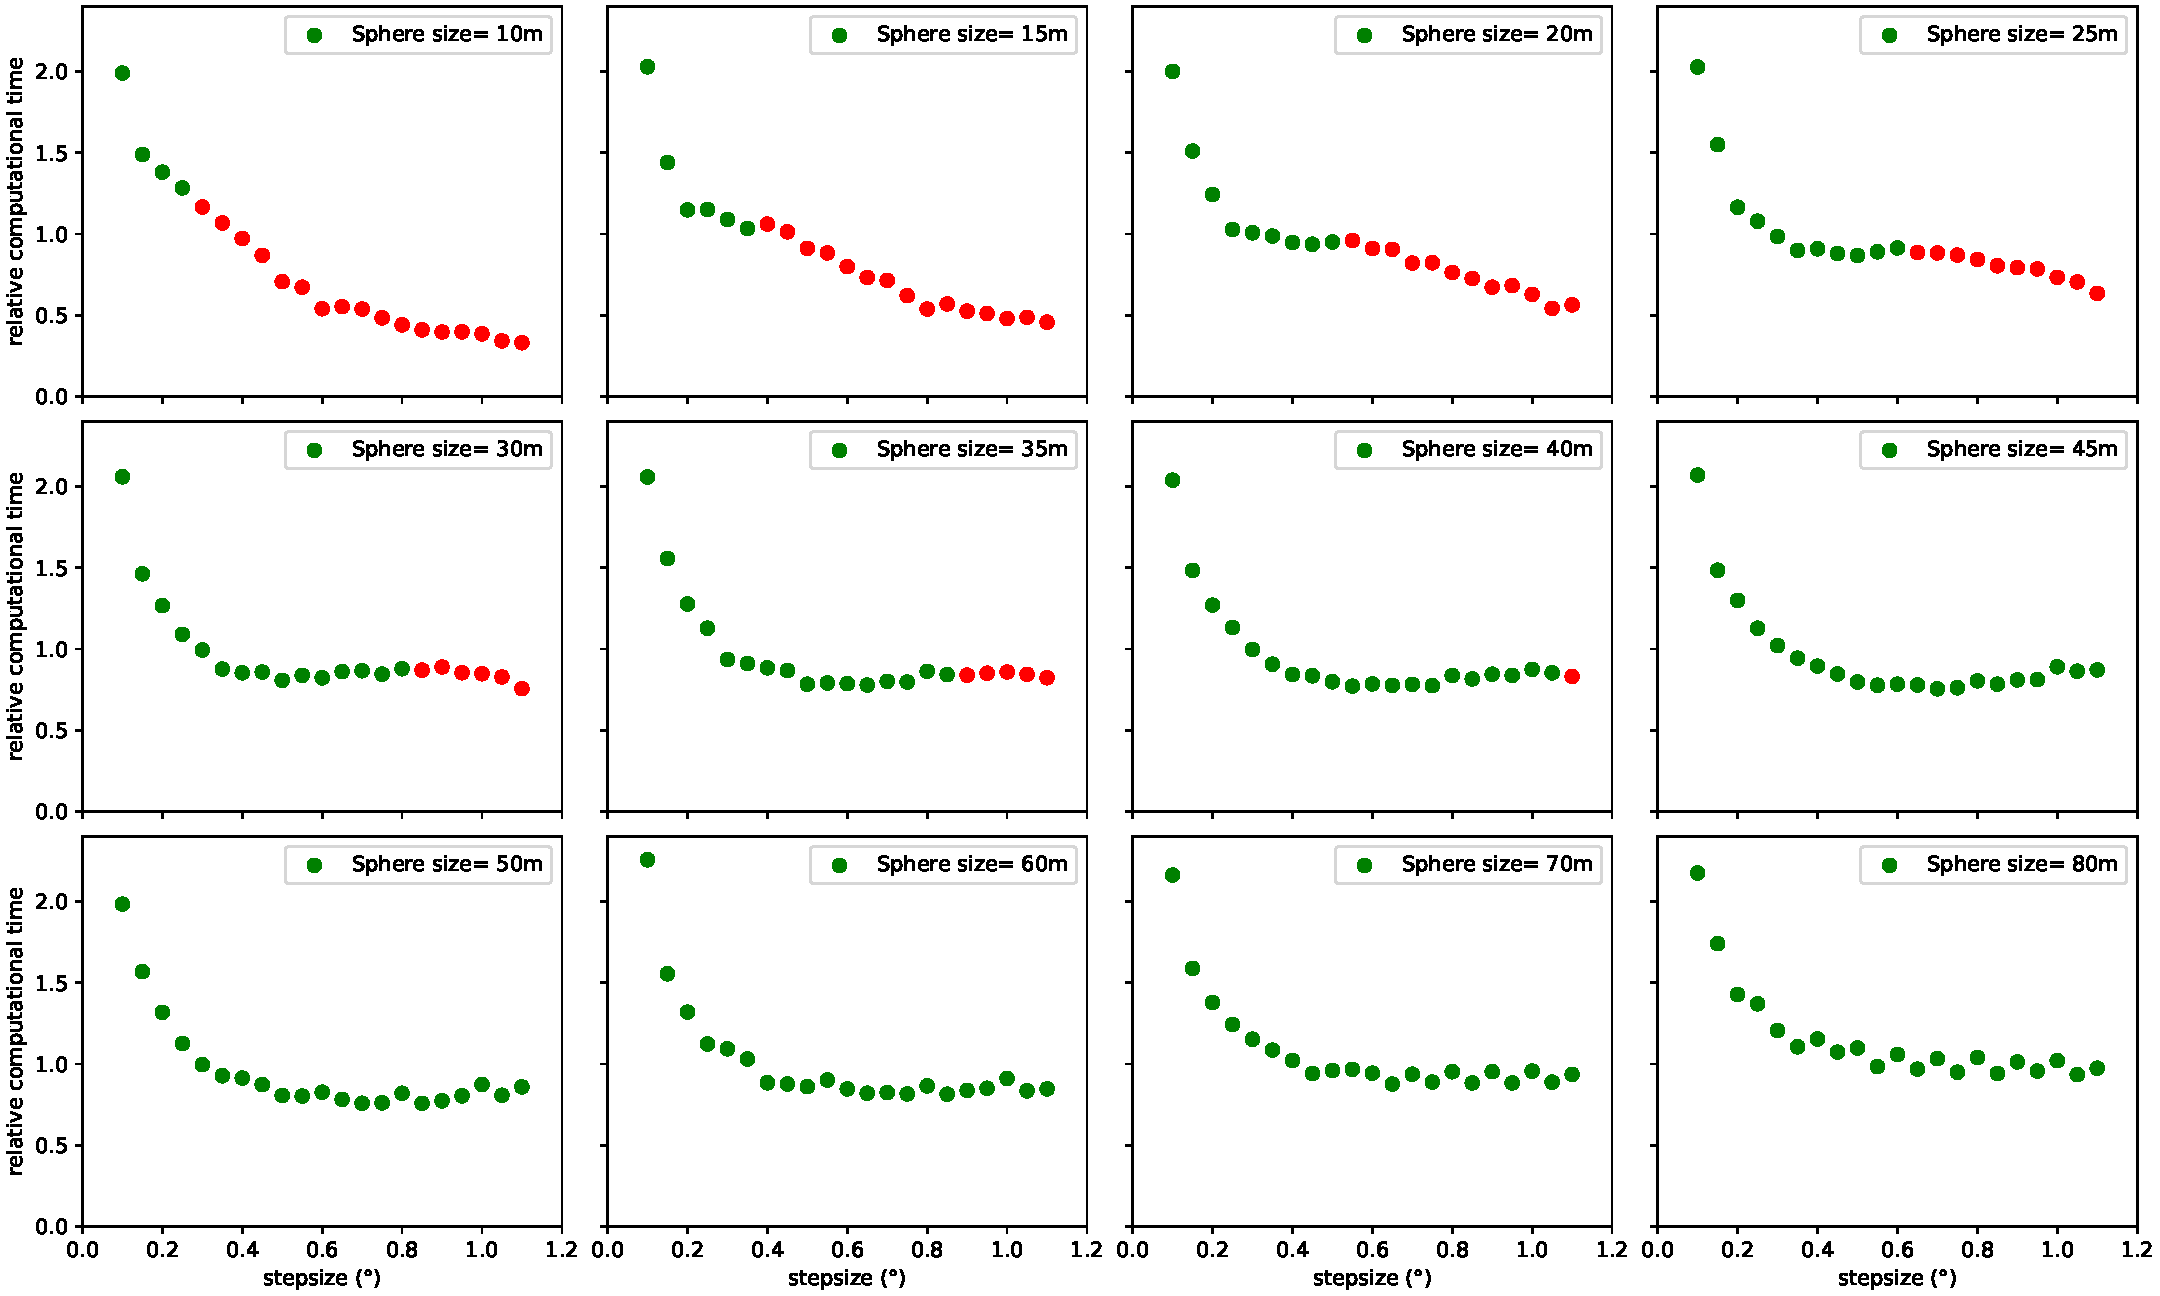
\includegraphics[width=\textwidth]{figures/subplotofallstepsphere.pdf}
	\caption{Variation in Sphere and angle step size with report on relative time.}
	\label{fig:SphereStepInfl}
\end{figure}

\begin{figure}
	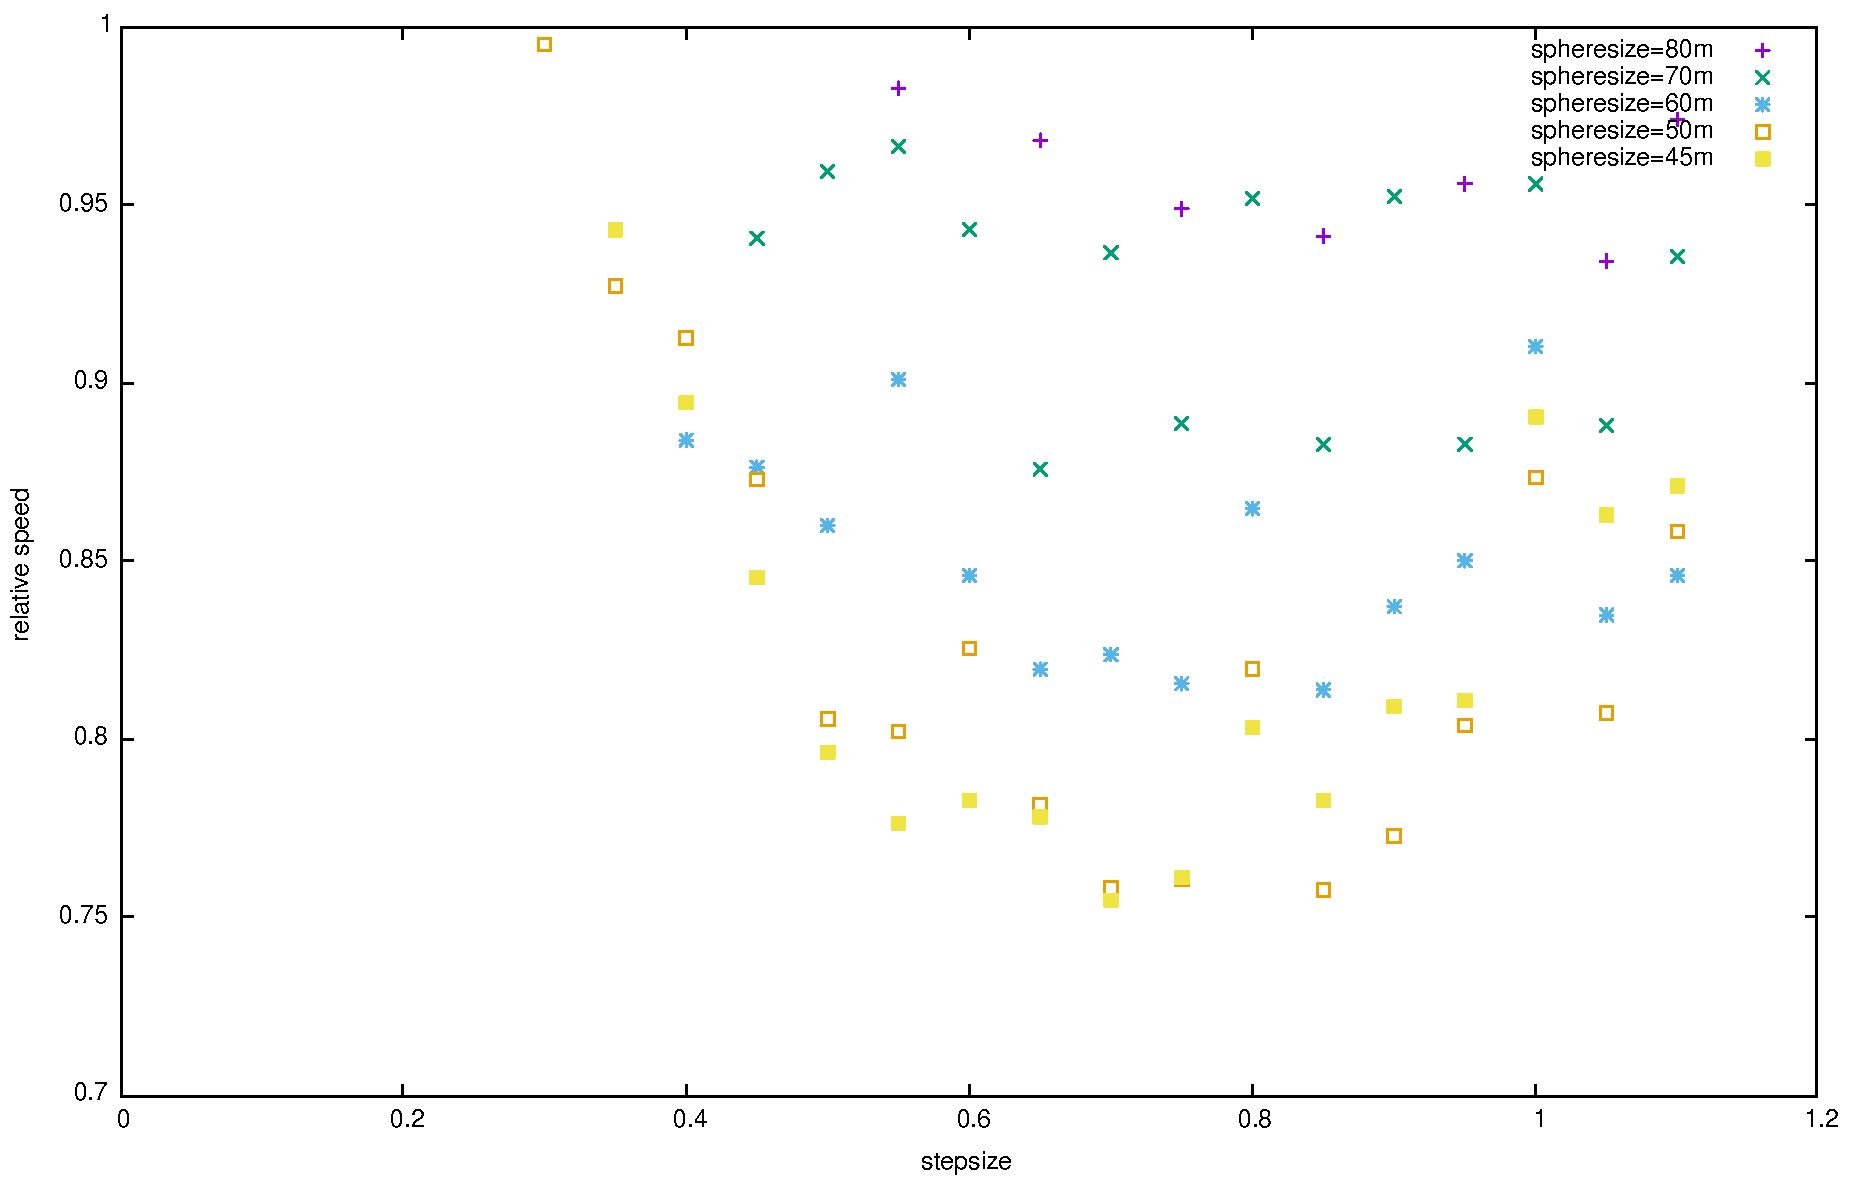
\includegraphics[width=\textwidth]{figures/SphereAndStepFinal.pdf}
	\caption{Green values in variation in sphere and angle step size with report on relative time.}
	\label{fig:SphereStepFinal}
\end{figure}

\chapter{Weather Balloon}
\label{chap:WB}
In this chapter we'll simulate radio signals coming from a weather
balloon flying over the stations. Our goal is to use the plane waves 
method to reconstruct the position of the weather balloon with the
timing information inferred from the detected radio signals in the
detectors.
If this is somewhat succesfull it can be used (as we'll get to
shortly) to find out the local index of refraction in the ice.

There are 2 changes that need to happen first to our algorithm for us to
be able to simulate this: The air observers needs to be hard removed
as to make a ray tracing possible from within the air to the
detector and second off, we'll need to implement secondaries.
The problem is essentially that a ray coming from the balloon 
propagates to the ice, refracting and reflecting and then one 
of the refracted rays hits the detector. 
The "primary" ray is concidered the reflected one 
so we adjusted the algorithm to look at the secondary that ends
closest to the detector and return that ray. What this has as
a consequence is that the "path" you get back is only the path
from when it "became" a secondary (so only the part below the ice)
but this can be easily fixed as the radio wave just propagates
straight from the balloon to the beginning of that ray,  making 
the full ray reconstructable by just assuming a line from the 
balloon to the "start" of the ray.

From this information the propagation time from the balloon to the ice $t$ 
can later be added to the time of the path in the ice by measuring the 
length $d$ of the drawn line from the balloon to the beginning of the recorded path, 
setting the speed of radio waves in air to c and then just adding $t = d/c$.
\section{Plane Wave Reconstruction}
Now having modified our ray tracer, the first problem we'll consider is
plane wave reconstruction of the original position, an example path
to some of the deep sensors is given in figure \ref{fig:Example
trajectory}
\begin{figure}
	\centering
	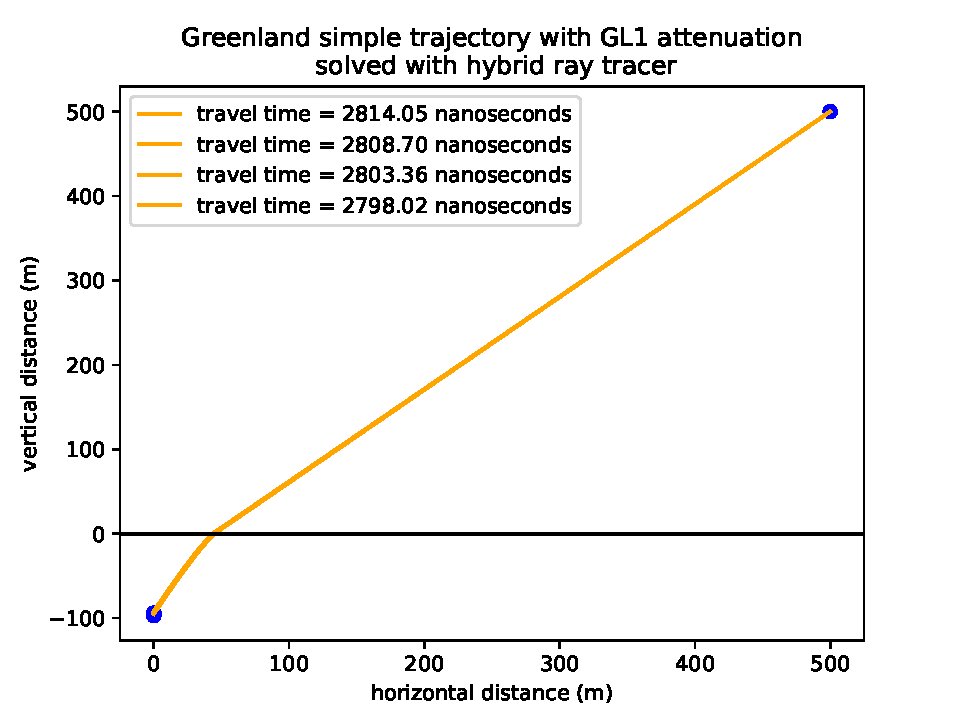
\includegraphics[width=0.7\textwidth]{weerballontraject.pdf}
	\caption{Example trajectory of rays coming from a weather balloon (blue dot top right) and going through the ice to the various detectors (blue dots bottom left)}
	\label{fig:Example trajectory}
\end{figure}
\begin{figure}
	\centering
	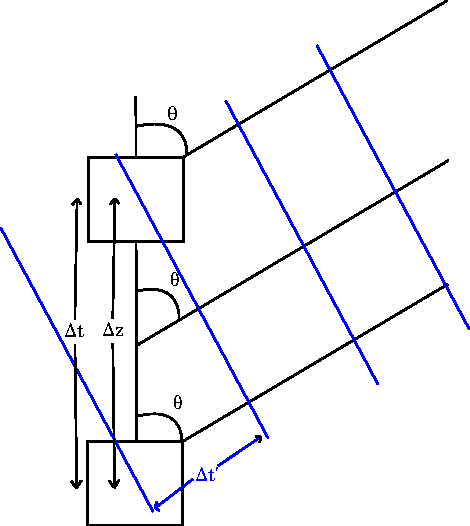
\includegraphics[width=0.7\textwidth]{planewave.pdf}
	\caption{Illustration of Plane waves}	
	\label{fig:Plane Wave}
\end{figure}
The plane wave reconstruction can easily be understood using figure
\ref{fig:Plane Wave}, the waves coming in are drawn in blue and
make a certain angle with the detectors. the top detector (top box)
detects the wave at a certain time $t_1$, the bottom detector
detects it at a time $t_2$. In our database, after decoding the
signal we'd thus see that these two detectors got a signal $\Delta t
= t_1 - t_2$ seconds apart from eachother. Now ideally this is
equal to the time $\Delta t'$ which is the time it took the wave
to propagate that distance which we can calculate from 
basic trigonometry and dimensional analysis:
\begin{equation}
	\Delta t' = \frac{m}{(m/s)} = (s/m)*m = v^{-1} * m = v^{-1} \cos\theta \Delta z
\end{equation}
With $v = c/n$ the local speed of light. As previously discussed this n is
depth-dependent and for comparison with the fitted index we'll be using the
models local index of refraction. Say we have 4 detectors at depths -94,-95,-96,-97,
this then would mean that we'll set the index of refraction at a depth of -95.5, 
exactly inbetween:
\begin{mintedbox}{python}
ice = medium.greenland_simple()
n_exact = ice.get_index_of_refraction(np.array[0,0,-95.5])
\end{mintedbox}
Now in reality we don't know the angle a priori, we'll only have the timing
information, so we'll perform a scan by minimizing something we define here as 
\textit{the correlation function}:
\begin{equation}
	Correlation(\theta) := \Delta t - \Delta t' = \Delta t
	- \frac{\cos\theta \Delta z}{v}
  \label{eqn:PlaneWave}
\end{equation}
If we have more than 1 detector however (which of course will be the case in RNO-G),
we'll need to specifiy various correlation functions.
E.g if we have four detectors labeled 0 to 3 we'll have to construct
correlation functions between detectors 0\&1, 0\&2, 0\&3, 1\&2, 1\&3 and 2\&3 .
As all of these correlation functions will have different
sizes we'll norm them as follows:
\begin{equation}
	Correlation_{Normed}(\theta) =
	\frac{Correlation(\theta)}{\int Correlation(\theta)\Delta
	\theta}
\end{equation}
An example of these correlation functions is shown in figure \ref{fig:NormedCorrelation}, 
notice how you can't differentiate between the correlation functions, this is only possible
because of the hybrid ray tracer having that high of a precision.
\begin{figure}
	\centering
	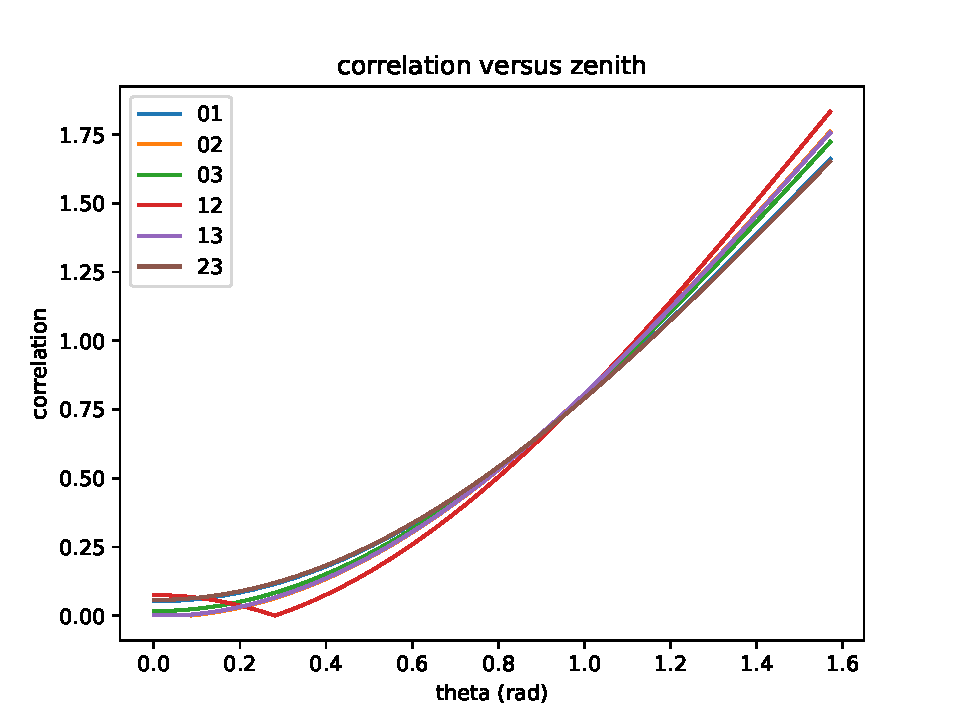
\includegraphics[width=0.8\textwidth]{NormedCorrelation.pdf}
	\caption{Example normed correlation functions}
	\label{fig:NormedCorrelation}
\end{figure}
\begin{figure}
	\centering
	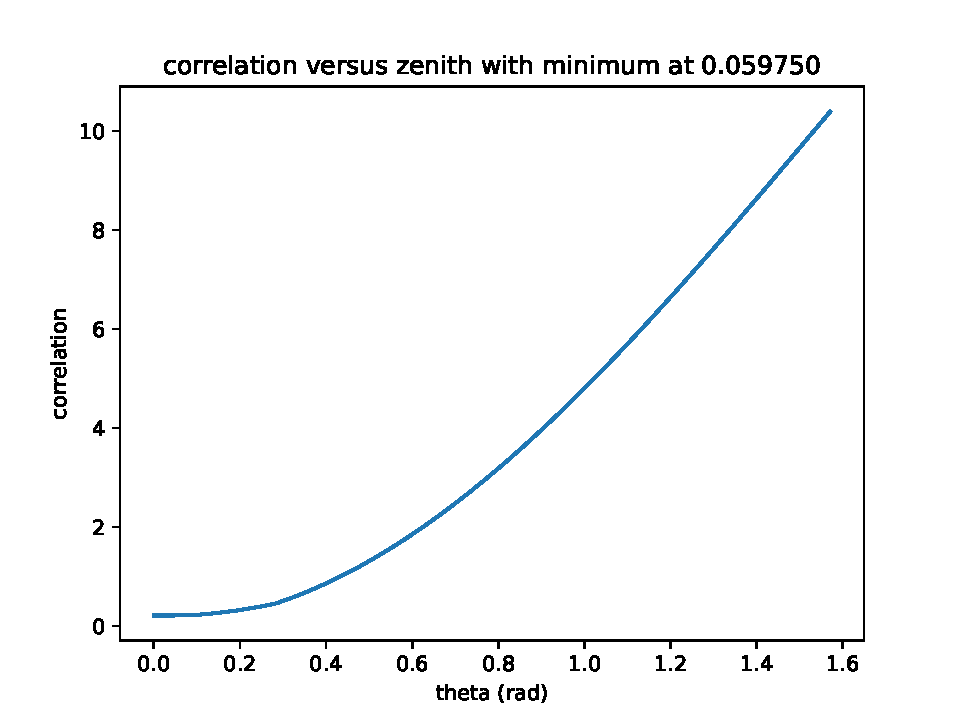
\includegraphics[width=\textwidth]{SummedCorrelation.pdf}
	\caption{Example sum of the normed correlation functions}
	\label{fig:SummedCorrelation}
\end{figure}
After this we can sum them, as shown in figure \ref{fig:SummedCorrelation}, and look
where it reaches it's minimum. Using this angle we can then reconstruct a ray and guess 
where the weather balloon is approximately, this is illustrated in figure 
\ref{fig:WeatherBalloonPositionReconstruction}. 
\section{Is the goal feasible?}
In the example reconstruction illustrated in figure
\ref{fig:WeatherBalloonPositionReconstruction} the difference in angle between
direct to balloon and plane wave reconstruction is already quite small
(0.65329617\%) but as the balloon gets closer to the detector this reduces
significantly as is shown in figure
\ref{fig:WeatherBalloonClosePositionReconstruction} where the difference in
angle between direct to balloon and plane wave reconstruction is only
0.06788141\%. Our goal is to find the local index of refraction n by using the
plane wave reconstruction with the recorded timing and the positional data from
the weather balloon as the plane wave reconstruction is heavily dependent on
the index of refraction (as can be seen in equation \ref{eqn:PlaneWave}). As
was already established we'll consider the index of refraction in the middle of
all the detectors (instead of a different one for every pair of detectors),
after experimenting this doesn't seem to have an impact on the accuracy of the
plane wave reconstruction. 

Now let's ask ourselves the question, within which angles should the
weather balloon fly for the data to be useful?  As was previously stated, the
further the weather balloon is away (in the x direction) the bigger the zenith
angle with the detector the less accurate the plane wave reconstruction.  So
which angles are acceptable? Note that not only angle but also height will eventually
play a role in the accuracy, the angle however gives a good starting point.
To determine this our method works as follows: 

we vary the position of the weather balloon in the x direction (keeping the
height constant), simulate the ray path to the channels 0 to 3 and then fit n
such that the difference between the reconstructed angle (from the plane wave
method) and the direct angle (angle between the middle of channels 0-3 and the
balloon) is the smallest possible.  Then we compare the n we have fit to the
one we know from the model at that position.  We quantise the discrepency
between these two indices of refraction using what we here define as the
\textit{relative accuracy}:
\begin{equation}
  \varepsilon\ (\%) = \frac{n_\text{fit} - n_{\text{exact}}}{n_{\text{exact}}} \times 100
\end{equation}
Carrying this out\footnote{The code for this can be found in projects-mt/BaLLooN/simulations as plane\_wave.py} we get figure \ref{fig:EpsilonIFODirect}, i.e it gets
exponentially shifted towards higher n as the balloon moves further away. If we wish our
accuracy to be within 1\%, the angle the balloon makes with the middle of channels 0 to 3 needs
to be less than 10°.
\begin{figure}
	\centering
	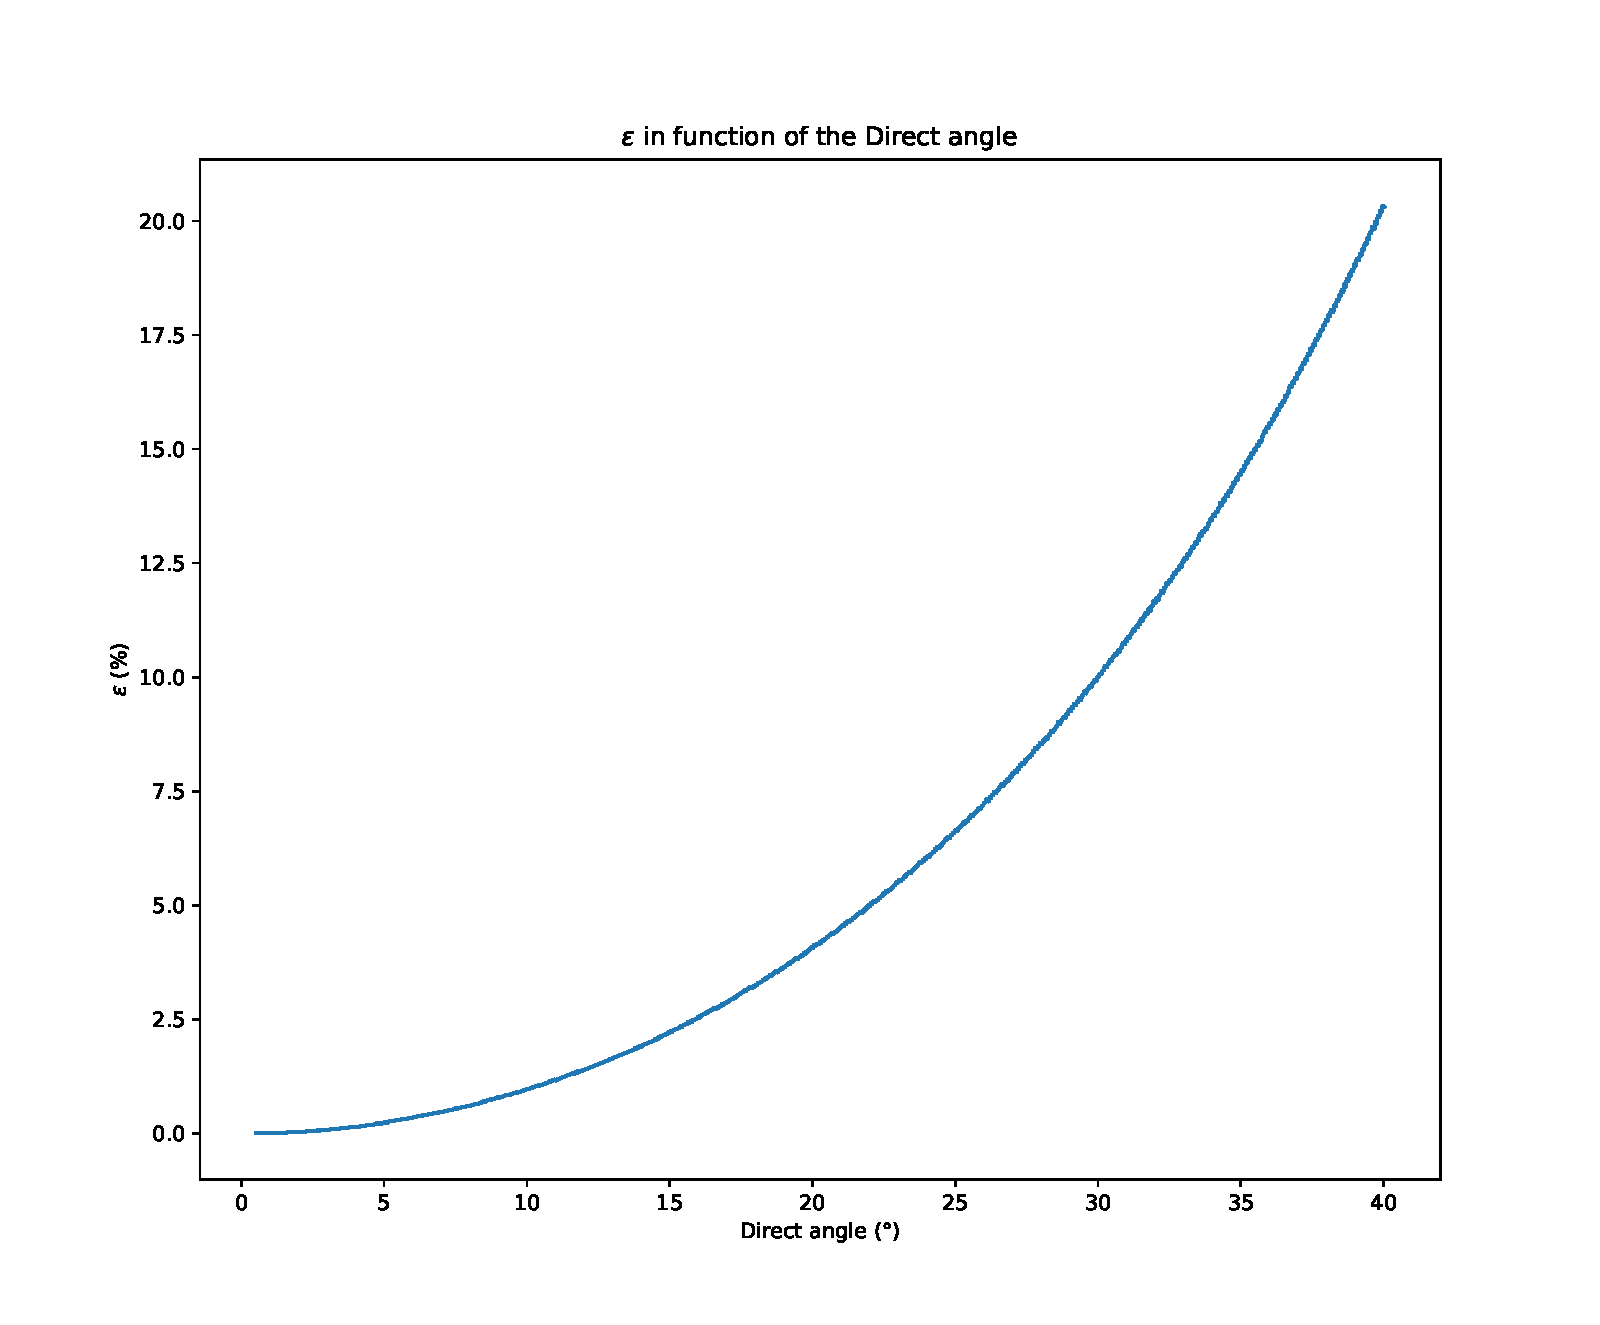
\includegraphics[width=0.7\textwidth]{EpsilonIFODirect.pdf}
	\caption{Epsilon in function of the direct angle}
	\label{fig:EpsilonIFODirect}
\end{figure}
\begin{figure}
  \centering
  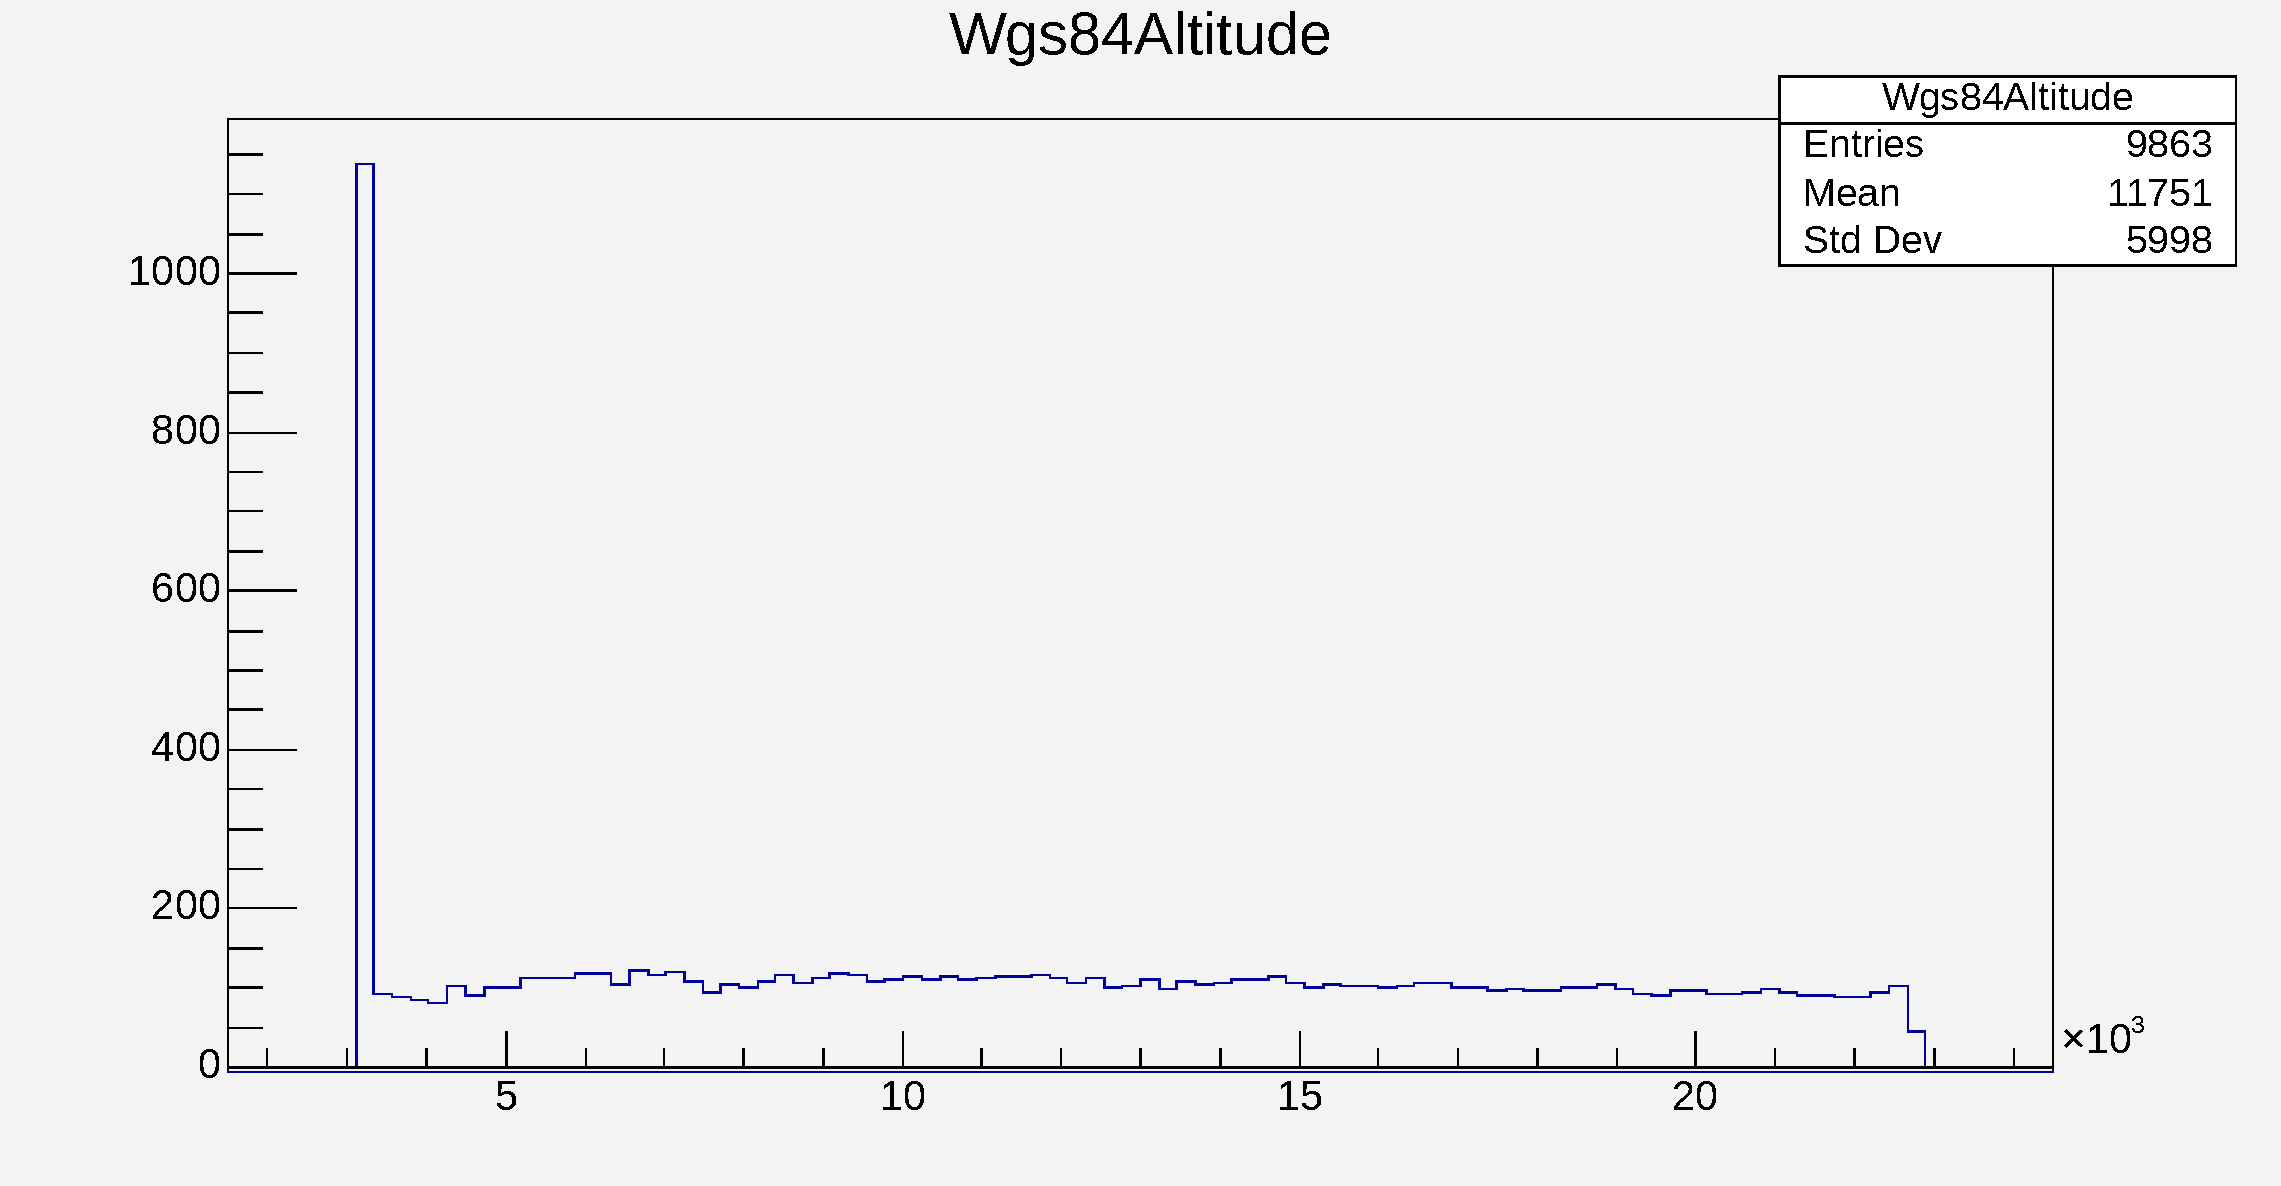
\includegraphics[width=0.7\textwidth]{BobsWeatherBalloonHeight.pdf}
  \caption{Height data viewed in ROOT}
  \label{fig:BobsWeatherBalloonHeight}
\end{figure}
An example path of a weather balloon is shown in figure
\ref{fig:ExampleBalloonPath}, looking specifically at the height information
recorded by the weather balloon in a .root file using
ROOT\footnote{\url{https://root.cern/}} we get what is shown in figure
\ref{fig:BobsWeatherBalloonHeight}. It can be seen that the elevation varies
between 3228m (read the graph as: Over a 1000 data entries at that height) and
22755m (entries go to zero after that height).  This is relative to sea-level,
looking at the height map of greenland as shown in figure
\ref{fig:HeightMapGreenland}
\begin{figure}
  \centering
  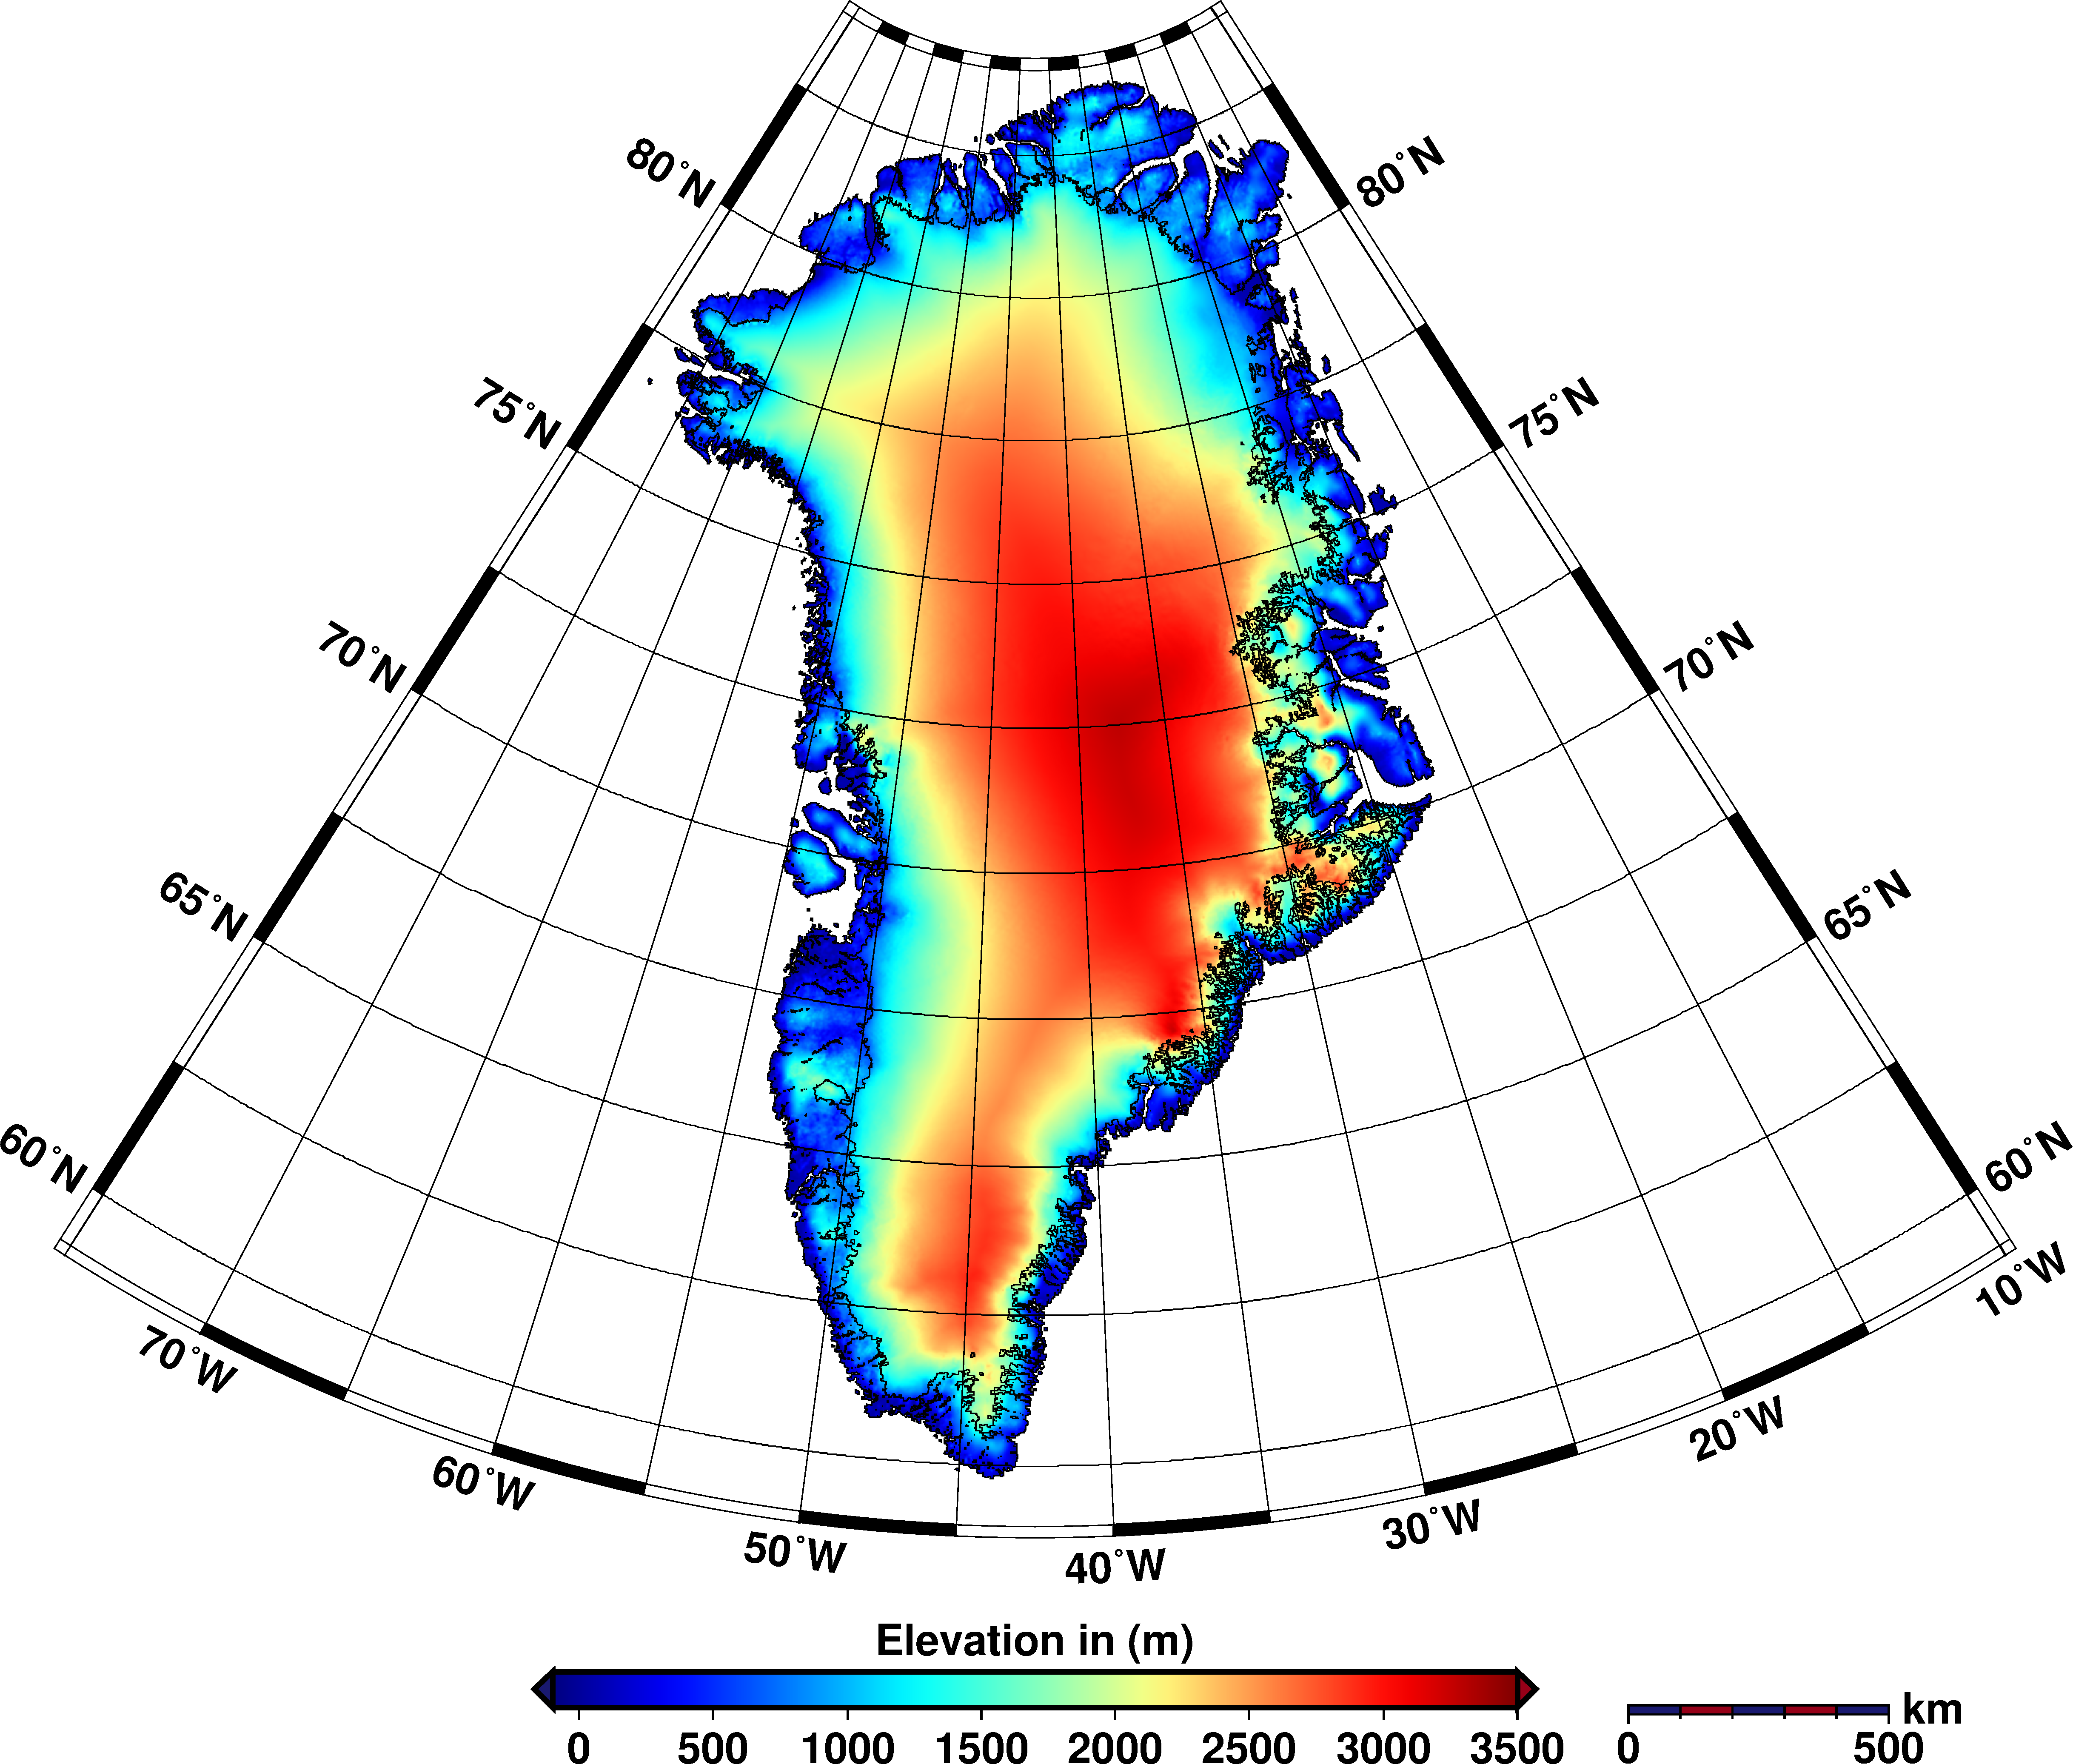
\includegraphics[width=0.4\textwidth]{GreenlandHeight.png}
  \caption{Height map of greenland}
  \label{fig:HeightMapGreenland}
\end{figure}
this is obvious.  It's quite difficult to work directly with the global geographic
coordinate system (longitudinal, latitude and elevation coordinates),
that's why we convert them to local ENU coordinates (north, east, up)
relative to the 'DISC' which is located at 72.58279265212887 latitude,
-38.45581495328228 longitude and 3251.9489147560234 elevation.

Now what would our $<$10° policy entail? And is it even possible? 
Say we take a look at station Terianniaq (station 12)
it's located at 72.6000868058195° N -38.4962265332872° W.
converting this into ENU coordinates we get -137.67250176003688N
1727.5184983294744E, we then set our "up" to be -95.5m as this is the
approximate location of the middle of channels 0-3.  Now looking at e.g the
Balloon path recorded on the 20th of august 2022 (figure
\ref{fig:ExampleBalloonPathCrossing12}) we see that the balloon crosses paths
closely with detector 12, but how close was this encounter? To quantize this we can take a look at every data
entry (there are $>$12000 entries) individually and compute the angle the
balloon makes with the detector by first converting the location of the balloon
in ENU coordinates, then calculating the horizontal distance ($\sqrt{(x-x')^2 +
(y-y')^2}$) then the relative vertical distance $|z - z'|$ and then from those
compute the angle ($tan(\theta) = \frac{Hor.}{Vert.}$) doing this and recording
when the balloon gets close enough to get below the 10° mark we get figure
\ref{fig:ExampleBalloonPathCrossing12LessThan10}. We thus see that in this
example the $<10$° policy is viable.

Now how much data do we have that way? 
We'll be looking at the data recorded over the summer of
2022, more particularly 15/06/2022 - 30/09/2022.
The positional data of the weather balloons was obtained from the
\url{ftp1.esrl.noaa.gov} website using the rno-g-sonde script of the official
RNO-G github page .After looping through every weather
balloon gpx file recorded in the summer of 2022 and seeing where it get's
within 10 degrees we get the data shown in appendix \ref{app:10Deg}, even
though this is quite a lot of data there's still another step that we could do
to broaden the amount of usable data.
\subsection{Refraction at the surface}
Up until now we have not used the property that waves refract at the surface as
we didn't want to assume anything, now say that we include refraction at the
surface for our plane wave reconstruction. This would mean that we'd follow
analogous steps as our previous analysis, i.e doing a plane wave reconstruction
from the difference in timing and trying to fit the index of refraction, only
now the plane wave abides with snell's law at the surface, going from n=1.27 to
n=1 and we'll need to minimize the horizontal distance from the ray at the
height of the balloon and the balloon, not the angle.  
The full algorithm thus goes as follows: We first reconstruct the
plane wave launch angle $\theta_1$ by minimizing the correlation function
previously defined, this gives us a function
\begin{equation}
	z = a_{InIce}*x + b_{InIce}
	\label{eqn:InIcePlaneWave}
\end{equation}
The outgoing zenith angle at the surface $\theta_2$ can be calculated from snell's law:
\begin{equation}
n_1 \sin{\theta_1} = n_2 \sin{\theta_2} \implies  \theta_2 = \sin^{-1}\left(\frac{n_1}{n_2}\sin{\theta_1}\right)
\end{equation}
from this we know the slope of the wave path $a_{InAir} = \tan\left({\frac{\pi}{2} -
\theta_2}\right)$ but not the offset, but this can easily be found from equation
\ref{eqn:InIcePlaneWave} as 
\begin{equation}
	z = 0 = a_{InIce}*x_{End} + b_{InIce} \implies x_{End} = -\frac{b_{InIce}}{a_{InIce}}
\end{equation}
and 
\begin{align}
	z = 0 = a_{InAir}*x_{End} + b_{InAir} \implies b_{InAir} &= -a_{InAir}*x_{End}
	\\&= a_{InAir}* \frac{b_{InIce}}{a_{InIce}}
\end{align}
Now that we have the function describing the "path of the plane wave"\footnote{we use double
quotes as to emphasize that this is a reconstruction method and not an actual wave} in the air 
we can find out the horizontal position at the height of the balloon as
\begin{equation}
	z = z_{Balloon} = a_{InAir}*x_{f} + b_{InAir} \implies x_f = \frac{z_{Balloon} - b_{InAir}}{a_{InAir}}
\end{equation}
and iteratively loop over possible indices of refraction, minimizing $|x_{Balloon} - x_f|$.

Doing this whilst looping over possible horizontal balloon positions, we get
the result shown in figure \ref{fig:EpsilonIFODirectSnell}\footnote{The code
for this can be found in projects-mt/BaLLooN/simulations as
plane\_wave\_with\_snell.py}
\begin{figure}
	\centering
	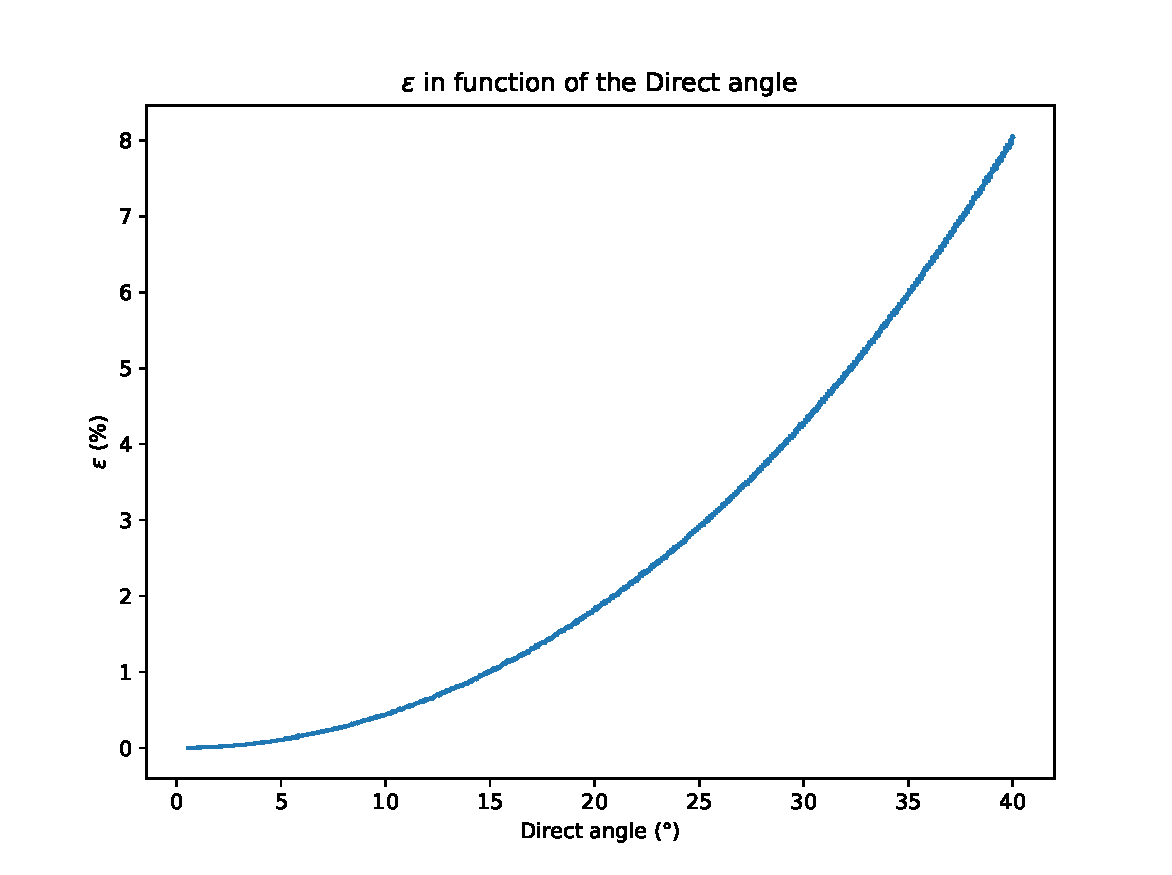
\includegraphics[width=0.7\textwidth]{EpsilonIFODirectSnell.pdf}
	\caption{epsilon IFO possible angles from channels 0-3 with refraction at the surface}
	\label{fig:EpsilonIFODirectSnell}
\end{figure}
As you can see we can now go up to 15° and still have less than 1\% error!  The
only drawback of this method is that we need to assume the index of refraction
to be 1.27 at the surface of the ice, if this isn't the case in some places our
predictions won't be accurate.
\begin{figure}
  \centering
	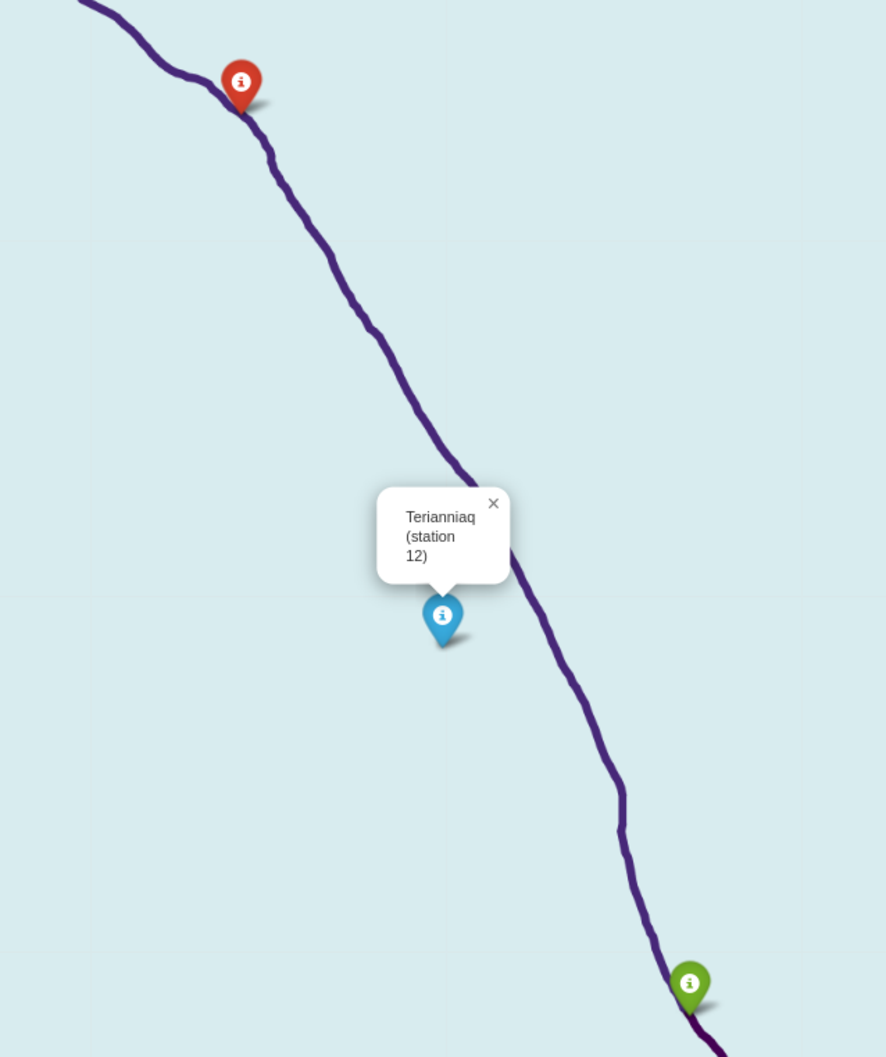
\includegraphics[width=0.7\textwidth]{StartAndStop10Illu.pdf}
  \caption{Illustration of when the angle with the deep array (channels 0-3) with the weather balloon is less than 10 degrees,
  the green mark indicates when it starts being less than 10 degrees and the red mark when it stops being less than 10 degrees.}
  \label{fig:ExampleBalloonPathCrossing12LessThan10}
\end{figure}

\begin{figure}
  \centering
	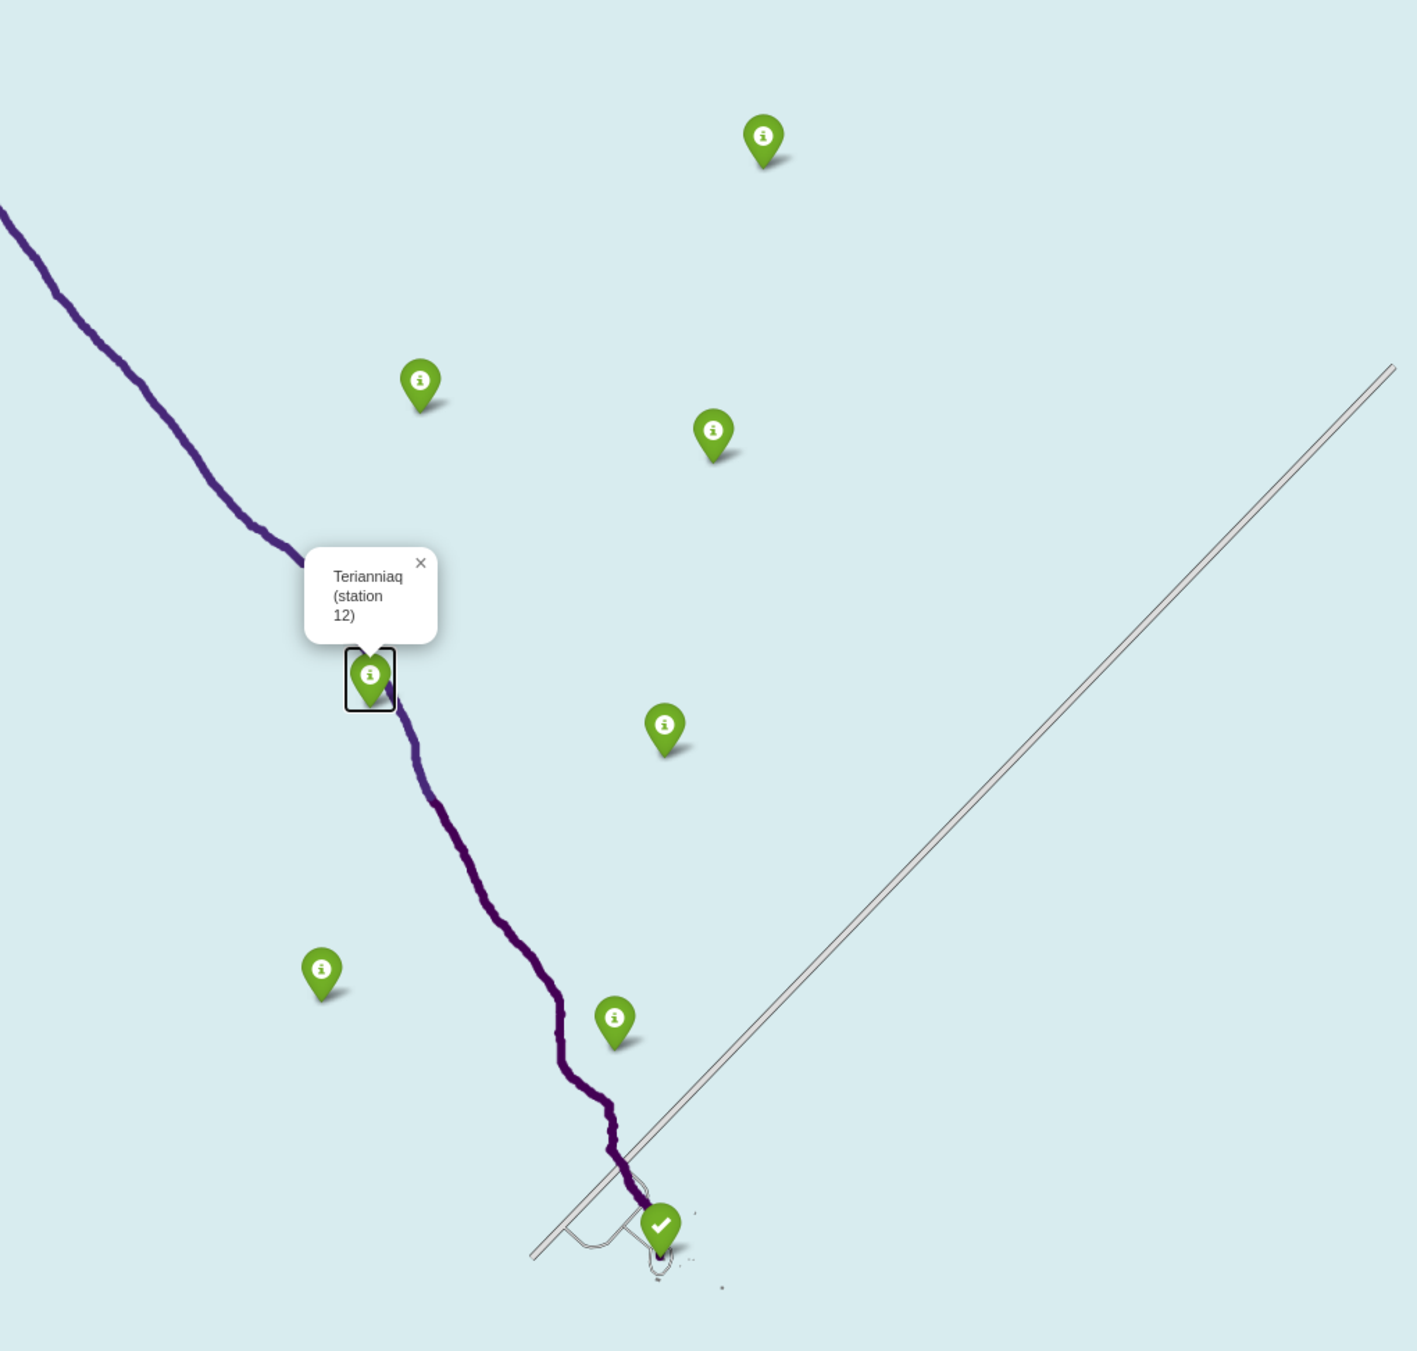
\includegraphics[width=0.7\textwidth]{PathSMT_20220820_111609.pdf}
  \caption{Path traced out by a weather balloon released at 20/08/2022}
  \label{fig:ExampleBalloonPathCrossing12}
\end{figure}
\begin{figure}
  \centering
	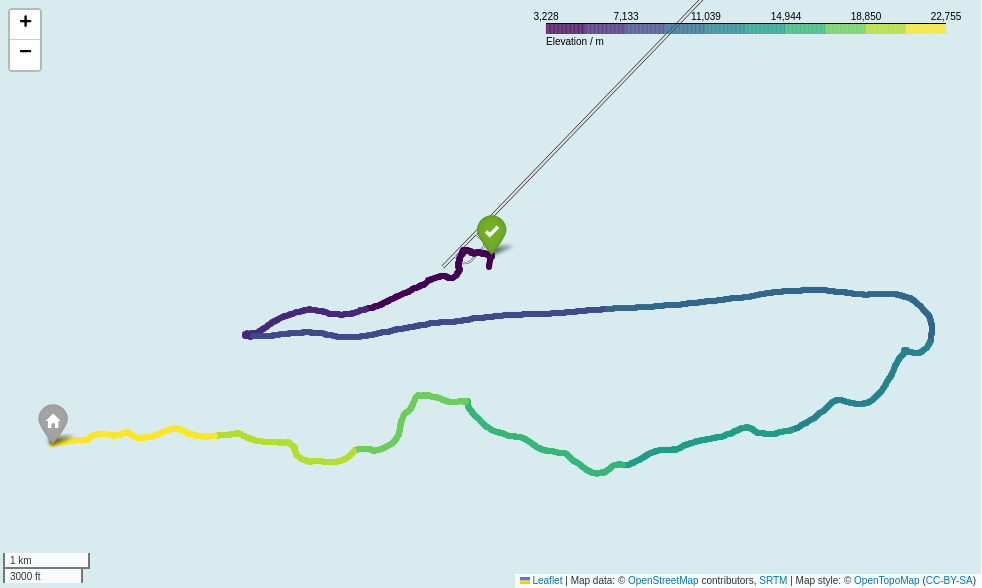
\includegraphics[width=0.7\textwidth]{WeatherBalloonPath.png}
  \caption{Path traced out by a weather balloon released by Bob Oeyen, the checkmark indicating the start and the house mark
  the end}
  \label{fig:ExampleBalloonPath}
\end{figure}

\begin{figure}
	\centering
	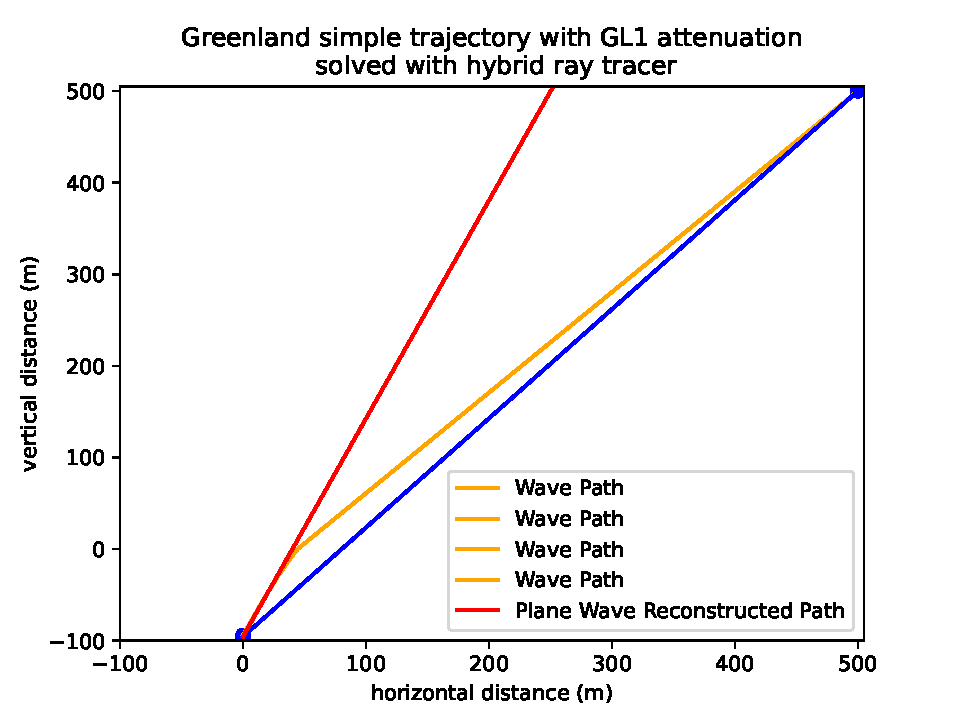
\includegraphics[width=0.9\textwidth]{WeatherBalloonPositionReconstruction.pdf}
	\caption{Example plane wave reconstruction of weather balloon position}
	\label{fig:WeatherBalloonPositionReconstruction}
\end{figure}
\begin{figure}
	\centering
	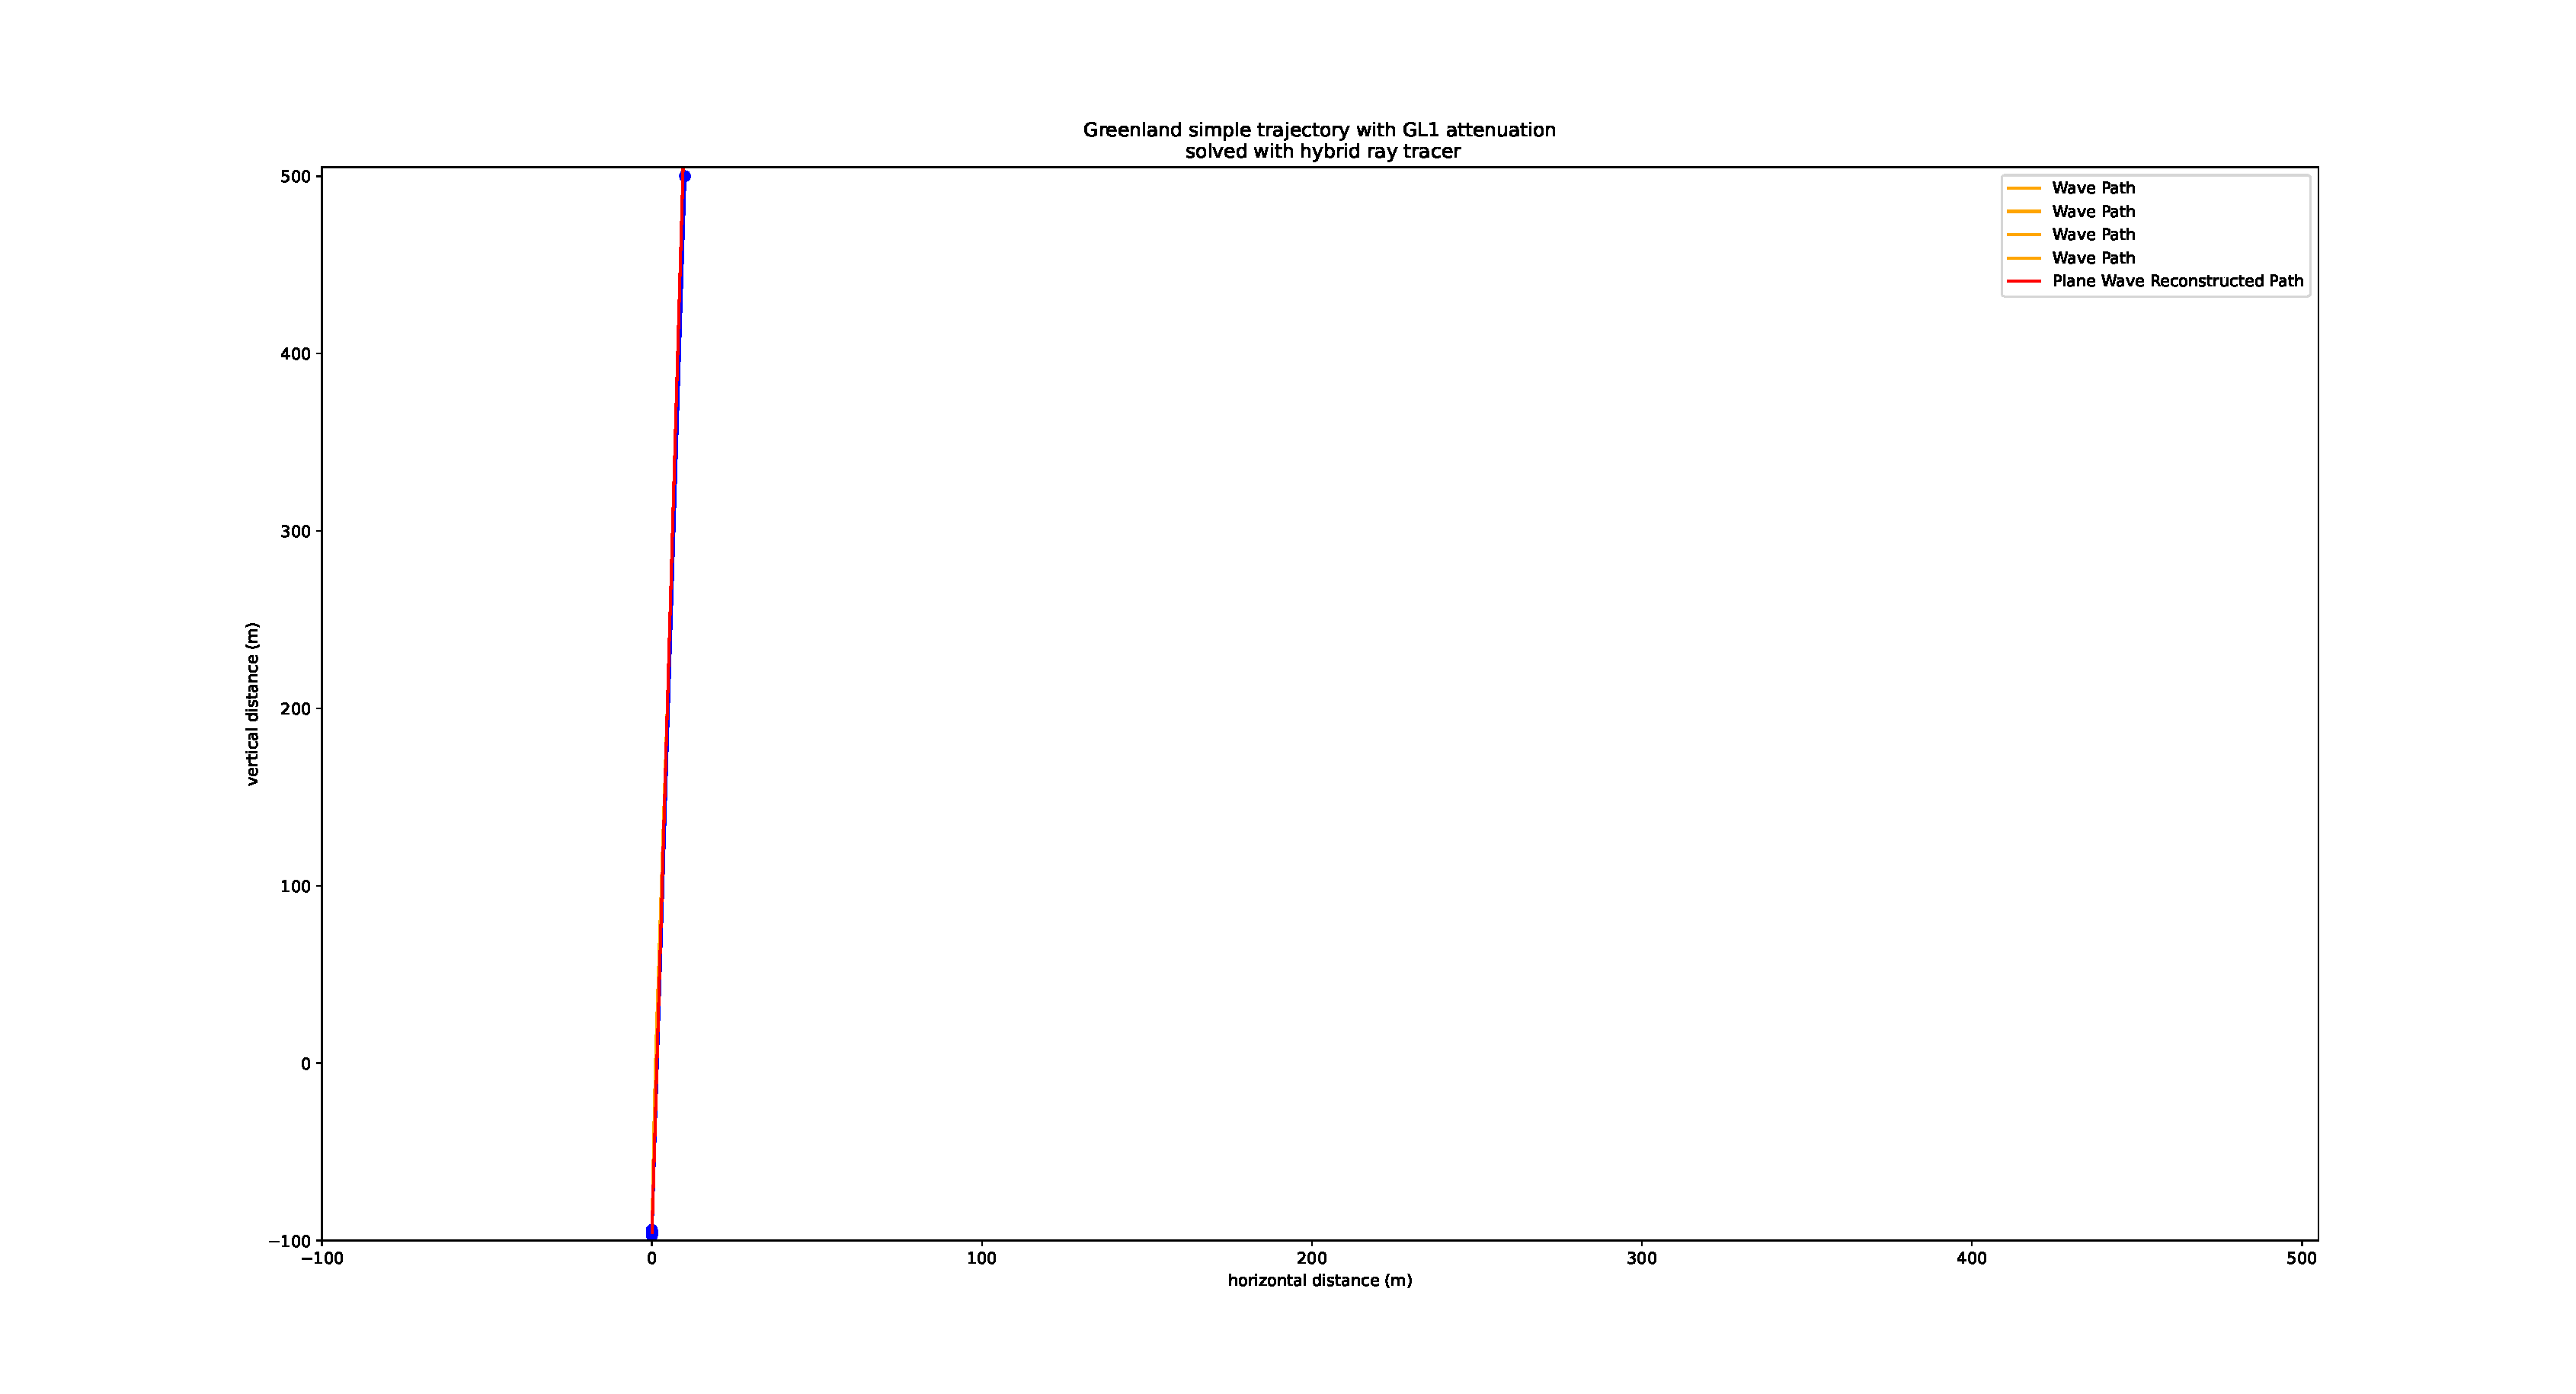
\includegraphics[width=0.9\textwidth]{WeatherBalloonClosePositionReconstruction.pdf}
	\caption{Example plane wave reconstruction of near-flying weather balloon position}
	\label{fig:WeatherBalloonClosePositionReconstruction}
\end{figure}
\newpage
\section{Error on prediction}
Running ahead on the actual measurements, let's estimate how accurate our
predictions will be.  For the moment we're only
interested in the deep channels 0-3. Let's label the vertical spatial accuracy,
i.e how accurately we know the height of these channels, $\delta z$\footnote{meaning if we have a measurement $z_i$ the true value is within $z_i
\pm \delta z$ with 95\% certainty}. And the timely accuracy, or how accurate the
vpol timing characteristics are, $\delta t$. If we want to fit n, we first
minimize the summed correlation function to construct the plane wave. One
correlation function is given by 
\begin{equation}
	Correlation(\theta) := \Delta t - \Delta t' = \Delta t
	- \frac{\cos\theta \Delta z}{v}
\end{equation}
Say the minimum occurs at $Correlation(\theta) = Correlation(\theta_{min}) := \mathcal{C}$, we can then re-write 
this equation for n:
\begin{equation}
  n = \frac{c(\Delta t - \mathcal{C})}{\cos \theta_{min} \Delta z} = \frac{c}{\cos{\theta_{min}}}\left[\frac{\Delta t}{\Delta z} - \frac{\mathcal{C}}{\Delta z}\right]
\end{equation}
The $\Delta z$ is the vertical distance between two channels and thus has an error of $2\delta z$ and $\Delta t$ is the time
difference between two channels, implying an error $2\delta t$. 
Let's look at the two terms seperately (assuming the error on $\theta_{min}$ to be negligable),
the first quotient $\phi_1 := \Delta t/\Delta z$ has a variance \cite{grabe2005measurement} of
\begin{equation}
	s_{\phi_1}^2 = \frac{1}{{\Delta z}^2}s_{\Delta t}^2 - 2 \frac{{\Delta t}}{{\Delta z}^3}s_{\Delta t \Delta z} + \frac{{\Delta t}^2}{{\Delta z}^4}s_{\Delta z}^2
\end{equation}
Assuming $\Delta t$ and $\Delta z$ to be independent:
\begin{align}
	s_{\phi_1}^2 &= \frac{1}{{\Delta z}^2}s_{\Delta t}^2 + \frac{{\Delta t}^2}{{\Delta z}^4}s_{\Delta z}^2\\
	&= 4\left(\frac{1}{{\Delta z}^2}{\delta t}^2 + \frac{{\Delta t}^2}{{\Delta z}^4}{\delta z}^2\right)
\end{align}
And the second term ($\phi_2 := -\mathcal{C}/\Delta z$):
\begin{align}
	s_{\phi_2}^2 &= \frac{\mathcal{C}^2}{{\Delta z}^2}s_{\Delta t}^2\\
		     &= 4\frac{\mathcal{C}^2}{{\Delta z}^2}{\delta t}^2\\
\end{align}
Our uncertainty on the index of refraction is thus (neglecting unknown systematic errors):
\begin{equation}
	\delta n =4\left(\frac{c}{\cos{\theta_{min}}}\right) \left( \frac{1}{{\Delta z}^2}{\delta t}^2 + \frac{{\Delta t}^2}{{\Delta z}^4}{\delta z}^2 + 
\frac{\mathcal{C}^2}{{\Delta z}^2}{\delta t}^2\right)
\end{equation}
%As we actually summed the correlation functions (6 in total), it's equivalent
%to doing 6 independent measurements of n, meaning that we get a reduction by a
%factor $\sim \sqrt{6}$.  
If we have more than 2 detectors, say N then the uncertainty on the fit can be assumed to be the
RMS of the individual uncertainties:
\begin{equation}
  \delta n =\sqrt{\sum_{i=0}^N \delta n _i^2}
\end{equation}
Let's assume $\epsilon$ to be an absolute error.  Now due to this inherent
inaccuracy, the "global" uncertainty on n also has an additional error of $\pm \epsilon(\vec{r})n$ with
$\vec{r}$ the position of the balloon.  Our final error on n is thus:
\begin{equation}
  \delta n(\vec{r})=  \epsilon(\vec{r})n + \sqrt{\sum_{i=0}^N \left[4\left(\frac{c}{\cos{\theta_{min}}}\right) \left( \frac{1}{{\Delta z_i}^2}{\delta t}^2 + \frac{{\Delta t_i}^2}{{\Delta z_i}^4}{\delta z}^2 + 
  \frac{\mathcal{C}^2}{{\Delta z_i}^2}{\delta t}^2\right)\right]^2 }
  \label{eqn:total error}
\end{equation}
%If we assume the $\epsilon$ to overestimate the index of refraction the same way in real
%life as in the simulation however, our estimated $n$ can be corrected as
%\begin{equation}
%  n_{\text{corrected}} (\vec{r})= \frac{n(\vec{r})}{\epsilon(\vec{r}) + 1}
%\end{equation}
%and our error becomes only the second part of equation \ref{eqn:total error}.
%As the error on the position of the channels is not yet fully known this whole
%section mainly serves as a future reference to calculate the errors on the
%indices of refraction that will be calculated in the next sections within
%this chapter.
\newpage
\section{Fitting the index: Channels 6 and 7}
Now that we know our goal to be feasible, let's analyse some data.  As we'll
start by just analysing one event, let's take one of the best events possible
for our analysis.  A close look at graph \ref{fig:EpsilonIFODirect} shows that
events under 5° at a height of 500m produce an error of less than 0.22\%,
implying that if we measure n to be 1.7407 our error will only be 0.0038. After
looping through all the balloon positional files and only outputting the $<5°$
ones we get some moments where balloons were actually close enough (note that
$<5°$ almost never happens at low heights).

If we search in the DESY database
\footnote{\url{https://rnog-monitor.zeuthen.desy.de/}} within the calculated
timeframes for the particular detectors where the balloon gets close enough to,
AND where the 403MHz signal coming from the Ballon (see figure
\ref{fig:BalloonFreq}) is detected in the deep channels, the events of the 29th
of august stands out; between 11:18:46 and 11:18:56, the balloon gets really
close to detector 23 as can be seen on figure \ref{fig:29/08/22}.
\begin{figure}
	\centering
	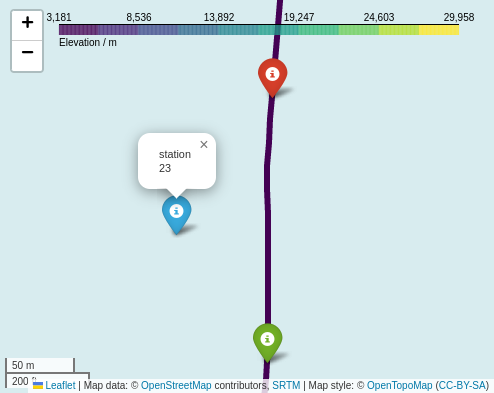
\includegraphics[width=0.4\textwidth]{29-08-Encounter.png}
	\caption{Close encounter between a weather balloon and detector 23 on the 29th of august 2022 at 11:18}
	\label{fig:29/08/22}
\end{figure}
If we take a look
at the detected signals we see that at run 691 the event 489 gets recorded at
2022-08-29 11:18:32+00:00 showing a clear 403MHz peak at channels 5-7.
It is of course unfortunate that we don't get to measure the index of refraction
at the deep component jet but a quick calculation shows that if we measure the
index of refraction using detectors 6 and 7 (getting the index of refraction at $\approx -50m$) 
the error will be $\approx 0.4\%$ which is a nice start\footnote{This calculation was
performed with the program CalculateInherentErrorWithSnell.py located in projects-mt/BaLLooN/RealData}.

Now to calculate the differences in timing for this received signal, the code
used for this is called FitN.py and stored at the repository
\href{https://github.com/arthuradriaens-code/projects-mt.git}{projects-mt}
under BaLLooN/RealData, let's go over the full code step by step:\footnote{I advise 
the people who will continue this work to pull up the code side-by-side with this 
explanation}

\subsection{Spatial data}
The first part we'll need to concern ourselves with is determining the relative
positions of everything. The balloon data file and the time when the event took
place are given, from these two both the latitudenal and longitudinal position
and elevation of the balloon at the given time is determined. We convert these
three measurements to the ENU coordinate frame and store it in the array
\textit{BalloonPosition}. The next step is to get the location of the detector,
for this we first instantiate a detector object 

\begin{mintedbox}{python}
det = NuRadioReco.detector.detector.Detector(json_file="RNO_season_2022.json")
\end{mintedbox}

The RNO season 2022 json file can be found on the official RNO-G github
under "analysis-tools", then we "update" the detector to the time of the event and get the
absolute position of our detector (station 23) via the get\_absolute\_position module:

\begin{mintedbox}{python}
	stationlocation = det.get_absolute_position(station_id)
\end{mintedbox}

Now that we have both the position of our balloon and station in ENU coordinates,
let's simplify the calculations by setting the detector as the origin.
i.e our new balloon position will be

\begin{equation}
	\textit{RelBalloon} = \textit{BalloonPosition} - \textit{StationPosition}
\end{equation}

And as we might want to plot this later, due to the cylindrical symmetry, we can rotate
the coordinates to get rid of our y-axis. We can do this by defining the radius:

\begin{equation}
	r := \sqrt{\textit{RelBalloon}_x^2 + \textit{RelBalloon}_y^2}
\end{equation}

and just setting this equal to $\textit{Balloon}_x$ and setting $\textit{Balloon}_y$ to
zero (equivalent to setting $\theta= 0$ in a rotation).

Now we don't have the position of our individual channels yet, only of the station itself,
these can however easily be obtained using the get\_relative\_position module on our
detector object, as we chose our station to be the center of the coordinate system,
these relative positions are absolute positions of the channels in our frame of reference.

\subsection{Signal analysis and initial guesses}
Now that we have our geometry, let's analyse the data for the channels 6 and 7,
the data for a particulal channel is stored in a channel object. From this
object we can get the recorded voltages with the get\_trace() module, the
recorded times with the get\_times() module, the recorded frequencies with the
get\_frequencies() and the recorded spectrum corresponding to these frequencies
with get\_frequency\_spectrum() , note that the last two do a FFT on our data.
The recorded spectrum of both channels is given in figure \ref{fig:freqs67}, we
observe a clear spike at 403.125MHz\footnote{The original signal of 403MHz gets binned
in 403.125MHz}.
\begin{figure}
	\begin{minipage}{0.49\textwidth}
		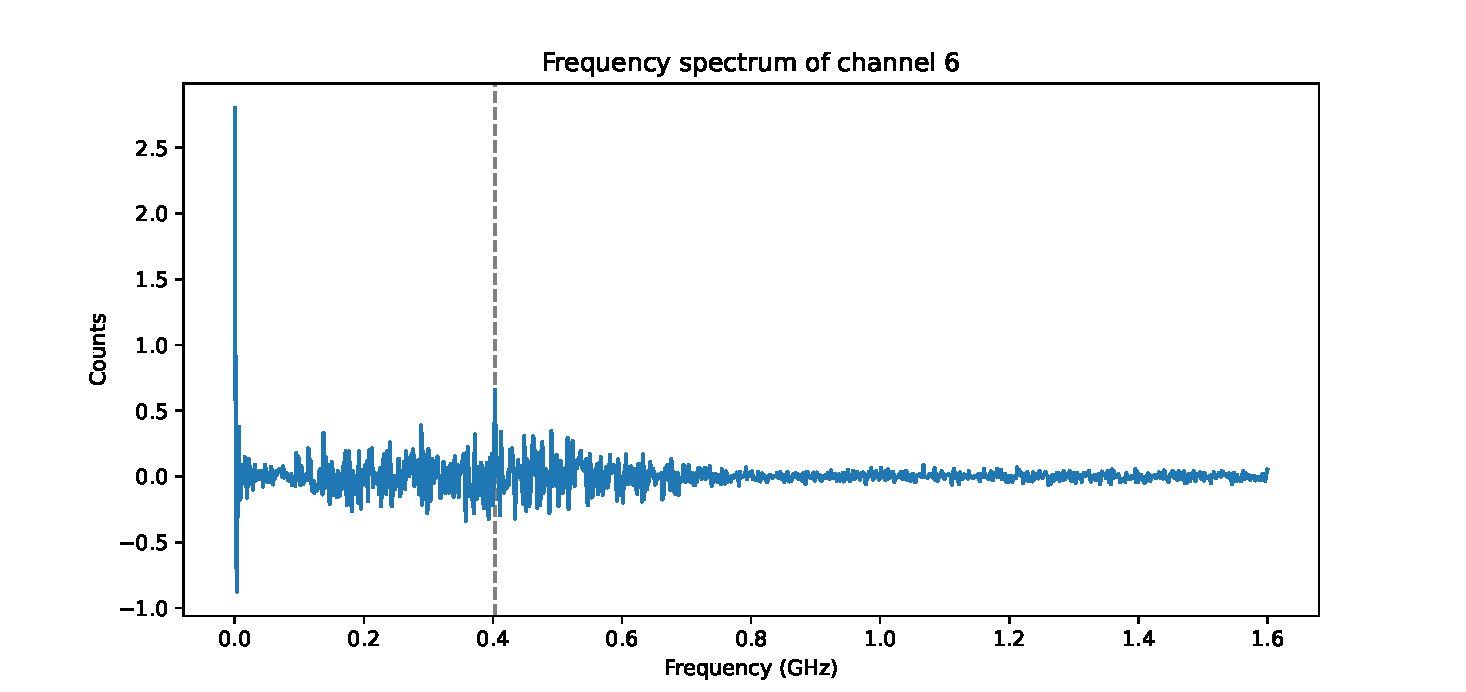
\includegraphics[width=\textwidth]{23-489-6-freq.pdf}
	\end{minipage}
	\begin{minipage}{0.49\textwidth}
		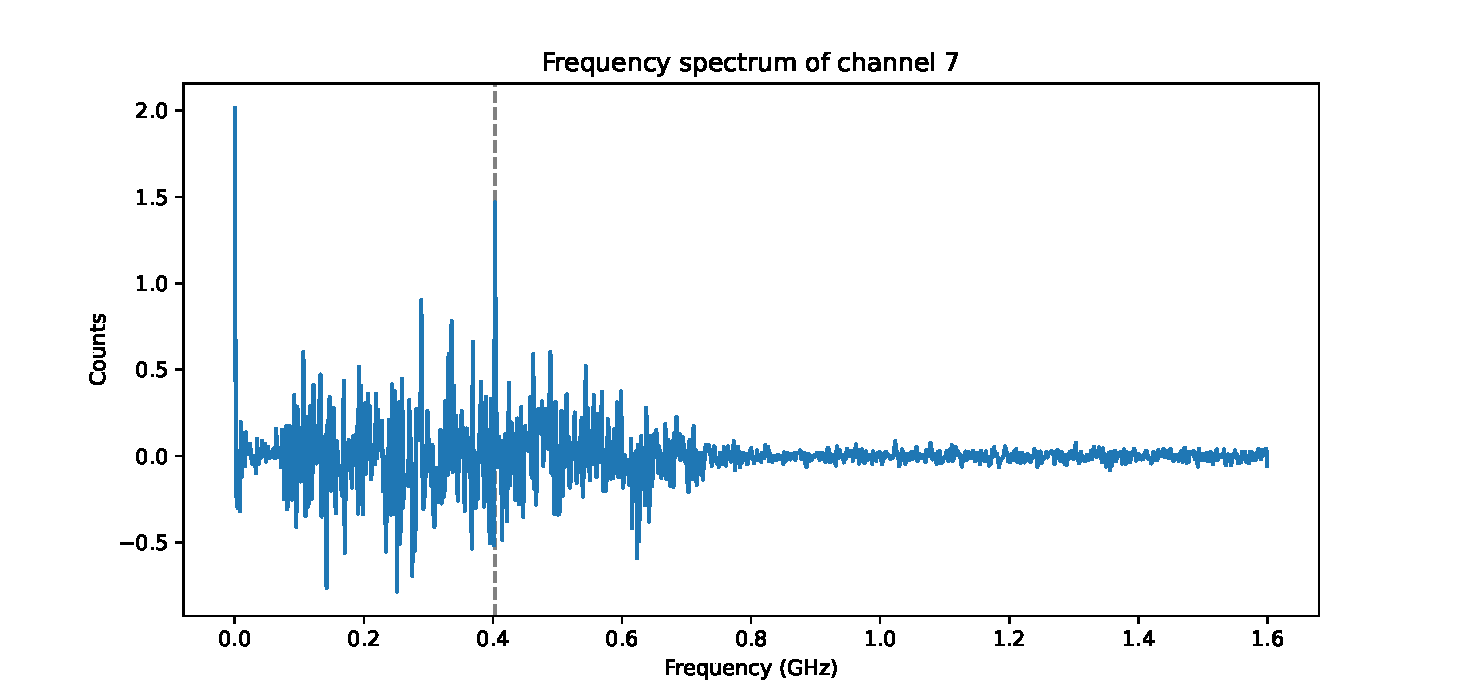
\includegraphics[width=\textwidth]{23-489-7-freq.pdf}
	\end{minipage}
	\caption{recorded frequencies on detector 23 at 2022/08/29 11:18:32}
	\label{fig:freqs67}
\end{figure}
We know that the signal sent out by the weather balloon has a "observed" frequency of
403.125MHz. As the data is measured in nanoseconds the frequency is:
\begin{equation}
	f = 403.125\text{MHz} = 403.125\times 10^{-3} \frac{1}{\text{ns}}
\end{equation}
Looking at the data in figure \ref{fig:voltage67} we see that we'll have to 
do some processing before fitting a sine of the form
\begin{equation}
	\mathcal{S} = A\cdot\sin\left(\omega t + T\right)
\end{equation}
with
\begin{equation}
	\omega = 2\pi f
\end{equation}
\begin{figure}
	\begin{minipage}{0.49\textwidth}
		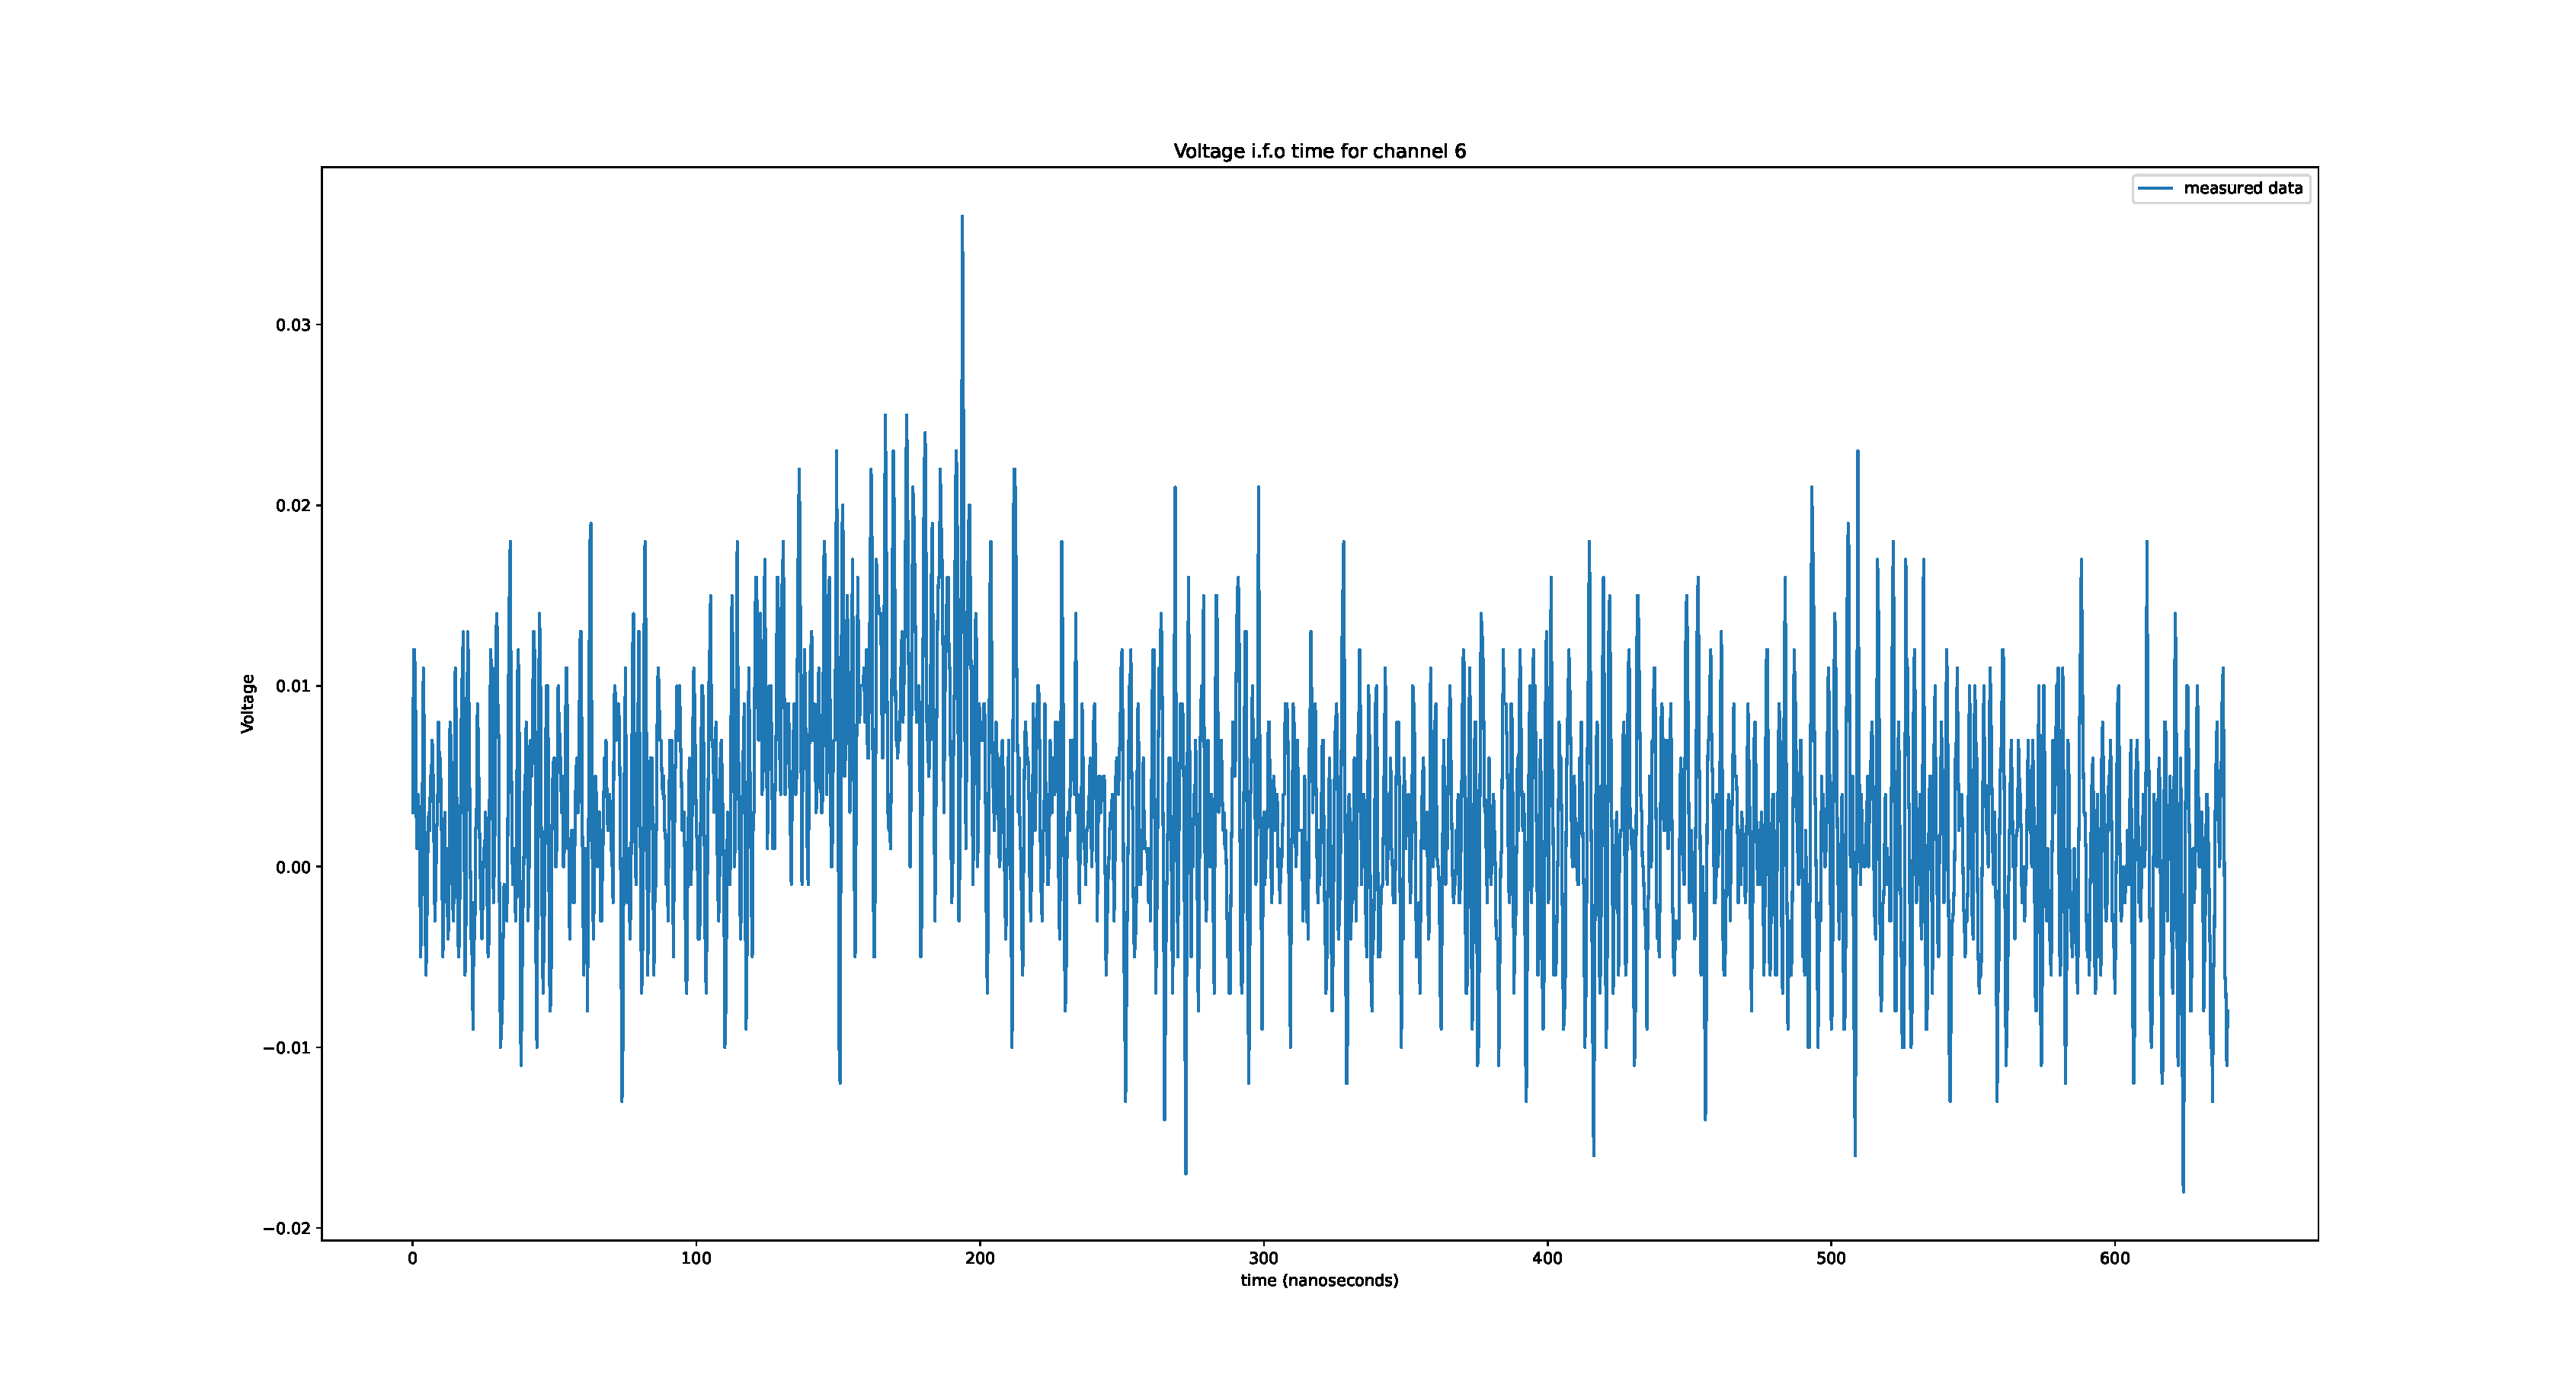
\includegraphics[width=\textwidth]{RawChannel6.pdf}
	\end{minipage}
	\begin{minipage}{0.49\textwidth}
		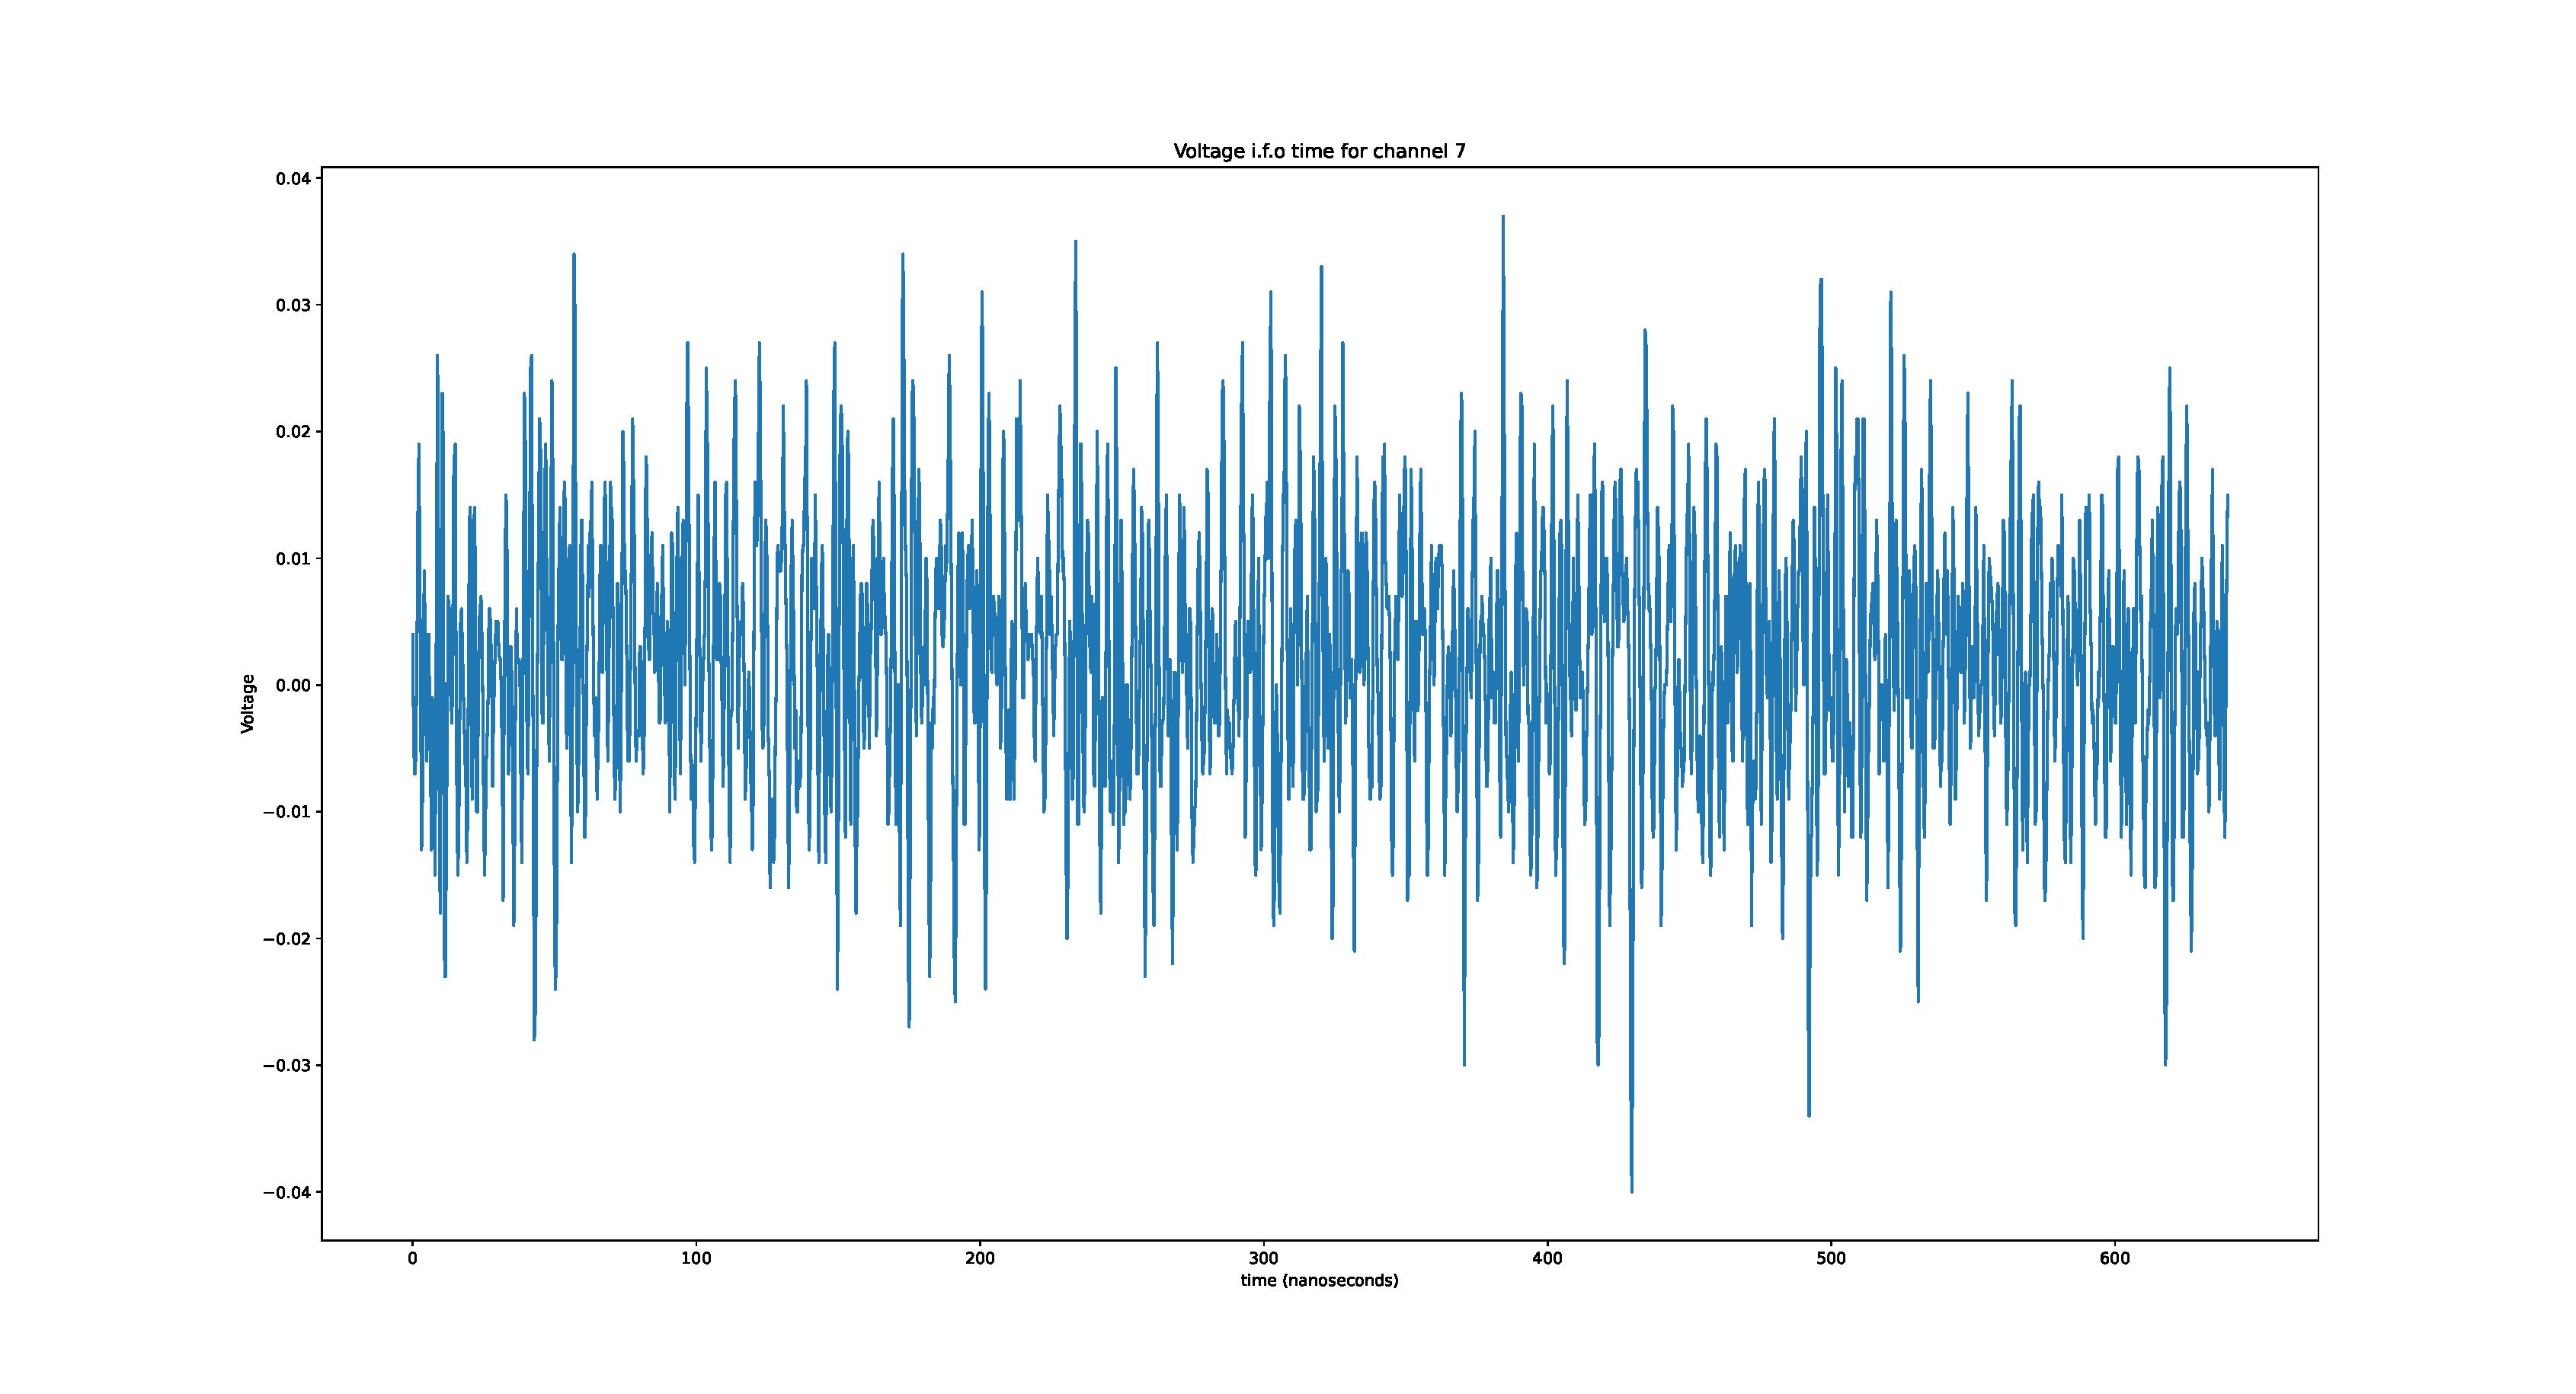
\includegraphics[width=\textwidth]{RawChannel7.pdf}
	\end{minipage}
	\caption{recorded voltage i.f.o time on detector 23 at 2022/08/29 11:18:32 for
	channels 6 and 7}
	\label{fig:voltage67}
\end{figure}
Let's first pass this signal through a sixth order butterworth filter with a
passband of [0.4031249, 0.4031251]\footnote{This is a filter that only let's
frequencies pass whom are within the passband, here it will let 0.403125 pass}. 
Doing this we notice that the signal looks as shown
in figure \ref{fig:ModulatedChannels}, where it's clear that even though the
balloon indeed sends out a sinusoidal 403MHz frequency, this signal is
amplitude modulated (AM).  Meaning that we have a sinusoidial
carrier signal $c(t)$:
\begin{equation}
  c(t) = A \sin(2\pi f_c t)
\end{equation}
with a message signal
\begin{equation}
  m(t) = Am \cos(2\pi f_m t + \phi)
\end{equation}
These two modulated together thus has the form
\begin{equation}
  V(t) = \left[1 + \frac{m(t)}{A}\right]c(t) = A\sin(2\pi f_c t)[1 + m\cos(2\pi f_m  t + \phi)]
\end{equation}
With a little correction that, due to the nature of observing the signal, there will be another phase:
\begin{equation}
  V(t) = A\sin(2\pi f_c t + \phi_1)[1 + m\cos(2\pi f_m  t + \phi_2)]
\end{equation}
Herein the carrier frequency is given by $f_c = 0.403125$ as previously
established but with the other parameters seemingly unknown which we'll have to
fit to the measured data.  We can, however, do some educated guesses which will
help the fitting algorithm.  The first guess we'll do is establish the maximum
value, as we have implemented an algorithm of finding the envelope functions
(in green and orange on figure \ref{fig:ModulatedChannels}), this is as simple
as calling the max function on the high envelope. Looking at our function this
max value corresponds to
\begin{equation}
  e_{highmax} = A(1 + m) := E_1
\end{equation}
The minimal value of our high envelope function corresponds to the minimal value of the message signal, due to symmetry
it's actually easier to just look at the absolute maximal values of the low envelope:
\begin{equation}
  |e_{lowmax}| = A(1-m) := E_2
\end{equation}
combining these two we get an equation for A and one for m:
\begin{align}
  m &= \frac{\frac{E_1}{E_2} - 1}{\frac{E_1}{E_2} + 1}\\
  A &= \frac{E_1}{1+m}\\
\end{align}
The frequency of the message signal can also be found from looking at the
difference between subsequent "bumps", these will be spaced some time T apart,
from which an initial guess for the message frequency can be found as $f_m =
1/T$. The only thing left to find is the phases $\phi_i$, we'll just fit these
with an initial smart guess, for which I'll first have to talk about cable
delays which we'll denote as $t^d$.
We get the delay for the individual channels with the get\_cable\_delay
module, these later on need to be substracted from the fit.

The difference in timing can be found from using the different $\phi$'s we will fit;
this is easy to see from the following example: Consider a sine wave 
\begin{equation}
  sin(\omega t)
\end{equation}
This reaches a certain value x after a time $t_x$:
\begin{equation}
  t_x = \frac{1}{\omega}\sin^{-1}(x)
\end{equation}
Now a sine wave with an offset of $-\phi$ 
\begin{equation}
  sin(\omega t - \phi)
\end{equation}
reaches this same x only after a time
\begin{equation}
  t_x = \frac{1}{\omega}\left(\sin^{-1}(x) + \phi\right)
\end{equation}
i.e a difference of $\phi/\omega$. 

Knowing this relationship is useful for finding an initial guess for $\phi$ as
the recorded travel times $T_i$ are of the form $T = -\phi/\omega - t^d$ and we
know that the travel times should be around 4200 ns from a simple simulation
using the greenland simple ice model, meaning that our guess for $\phi$ is in
the neighborhood of $-\omega(4200-t^d)$ and should give the smallest
correlation function; doing this for this example we get that the $\phi$ for
channel 6 should be -752, and channel 7 we give as initial guess the final fit
of channel 6 as this channel is higher and will thus have less travel time implying a
higher $\phi$ (the algorithm seems to fit the $\phi$ upwards).  Fitting this function
with the initial guesses you get what's shown on figure
\ref{fig:FittedVoltage67}, i.e a perfect fit on the data.
\begin{figure}
	\begin{minipage}{0.49\textwidth}
		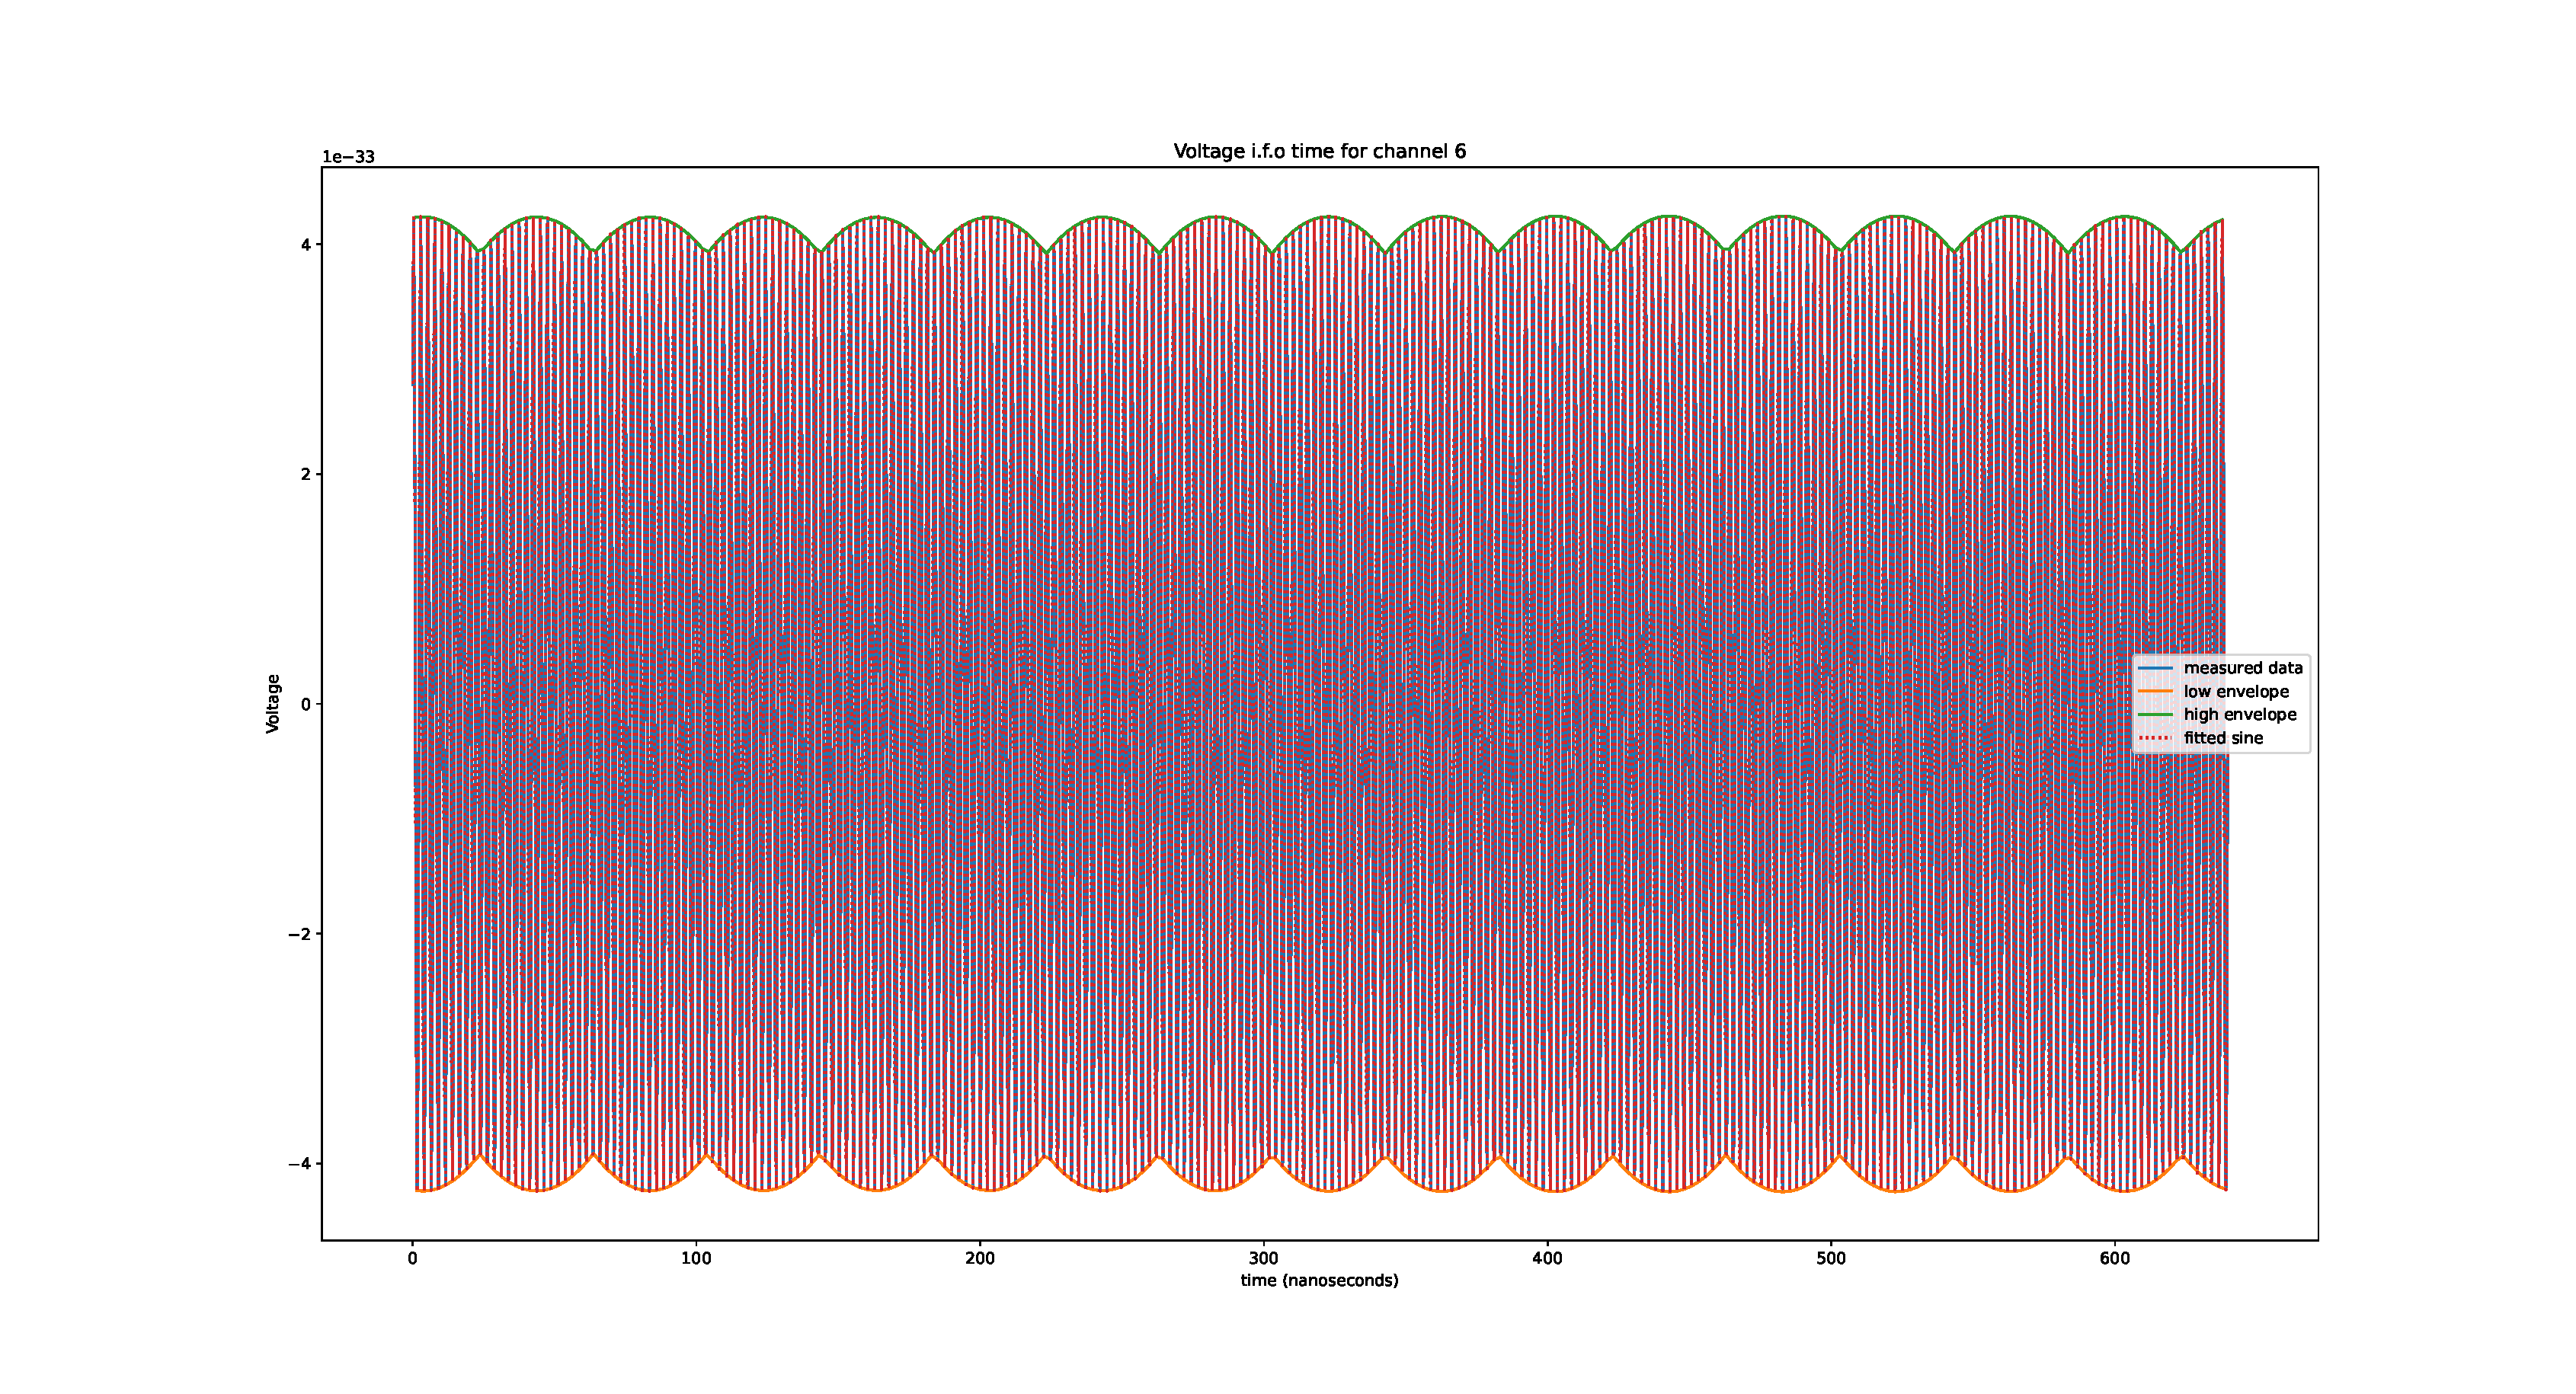
\includegraphics[width=\textwidth]{FitChannel6.pdf}
	\end{minipage}
	\begin{minipage}{0.49\textwidth}
		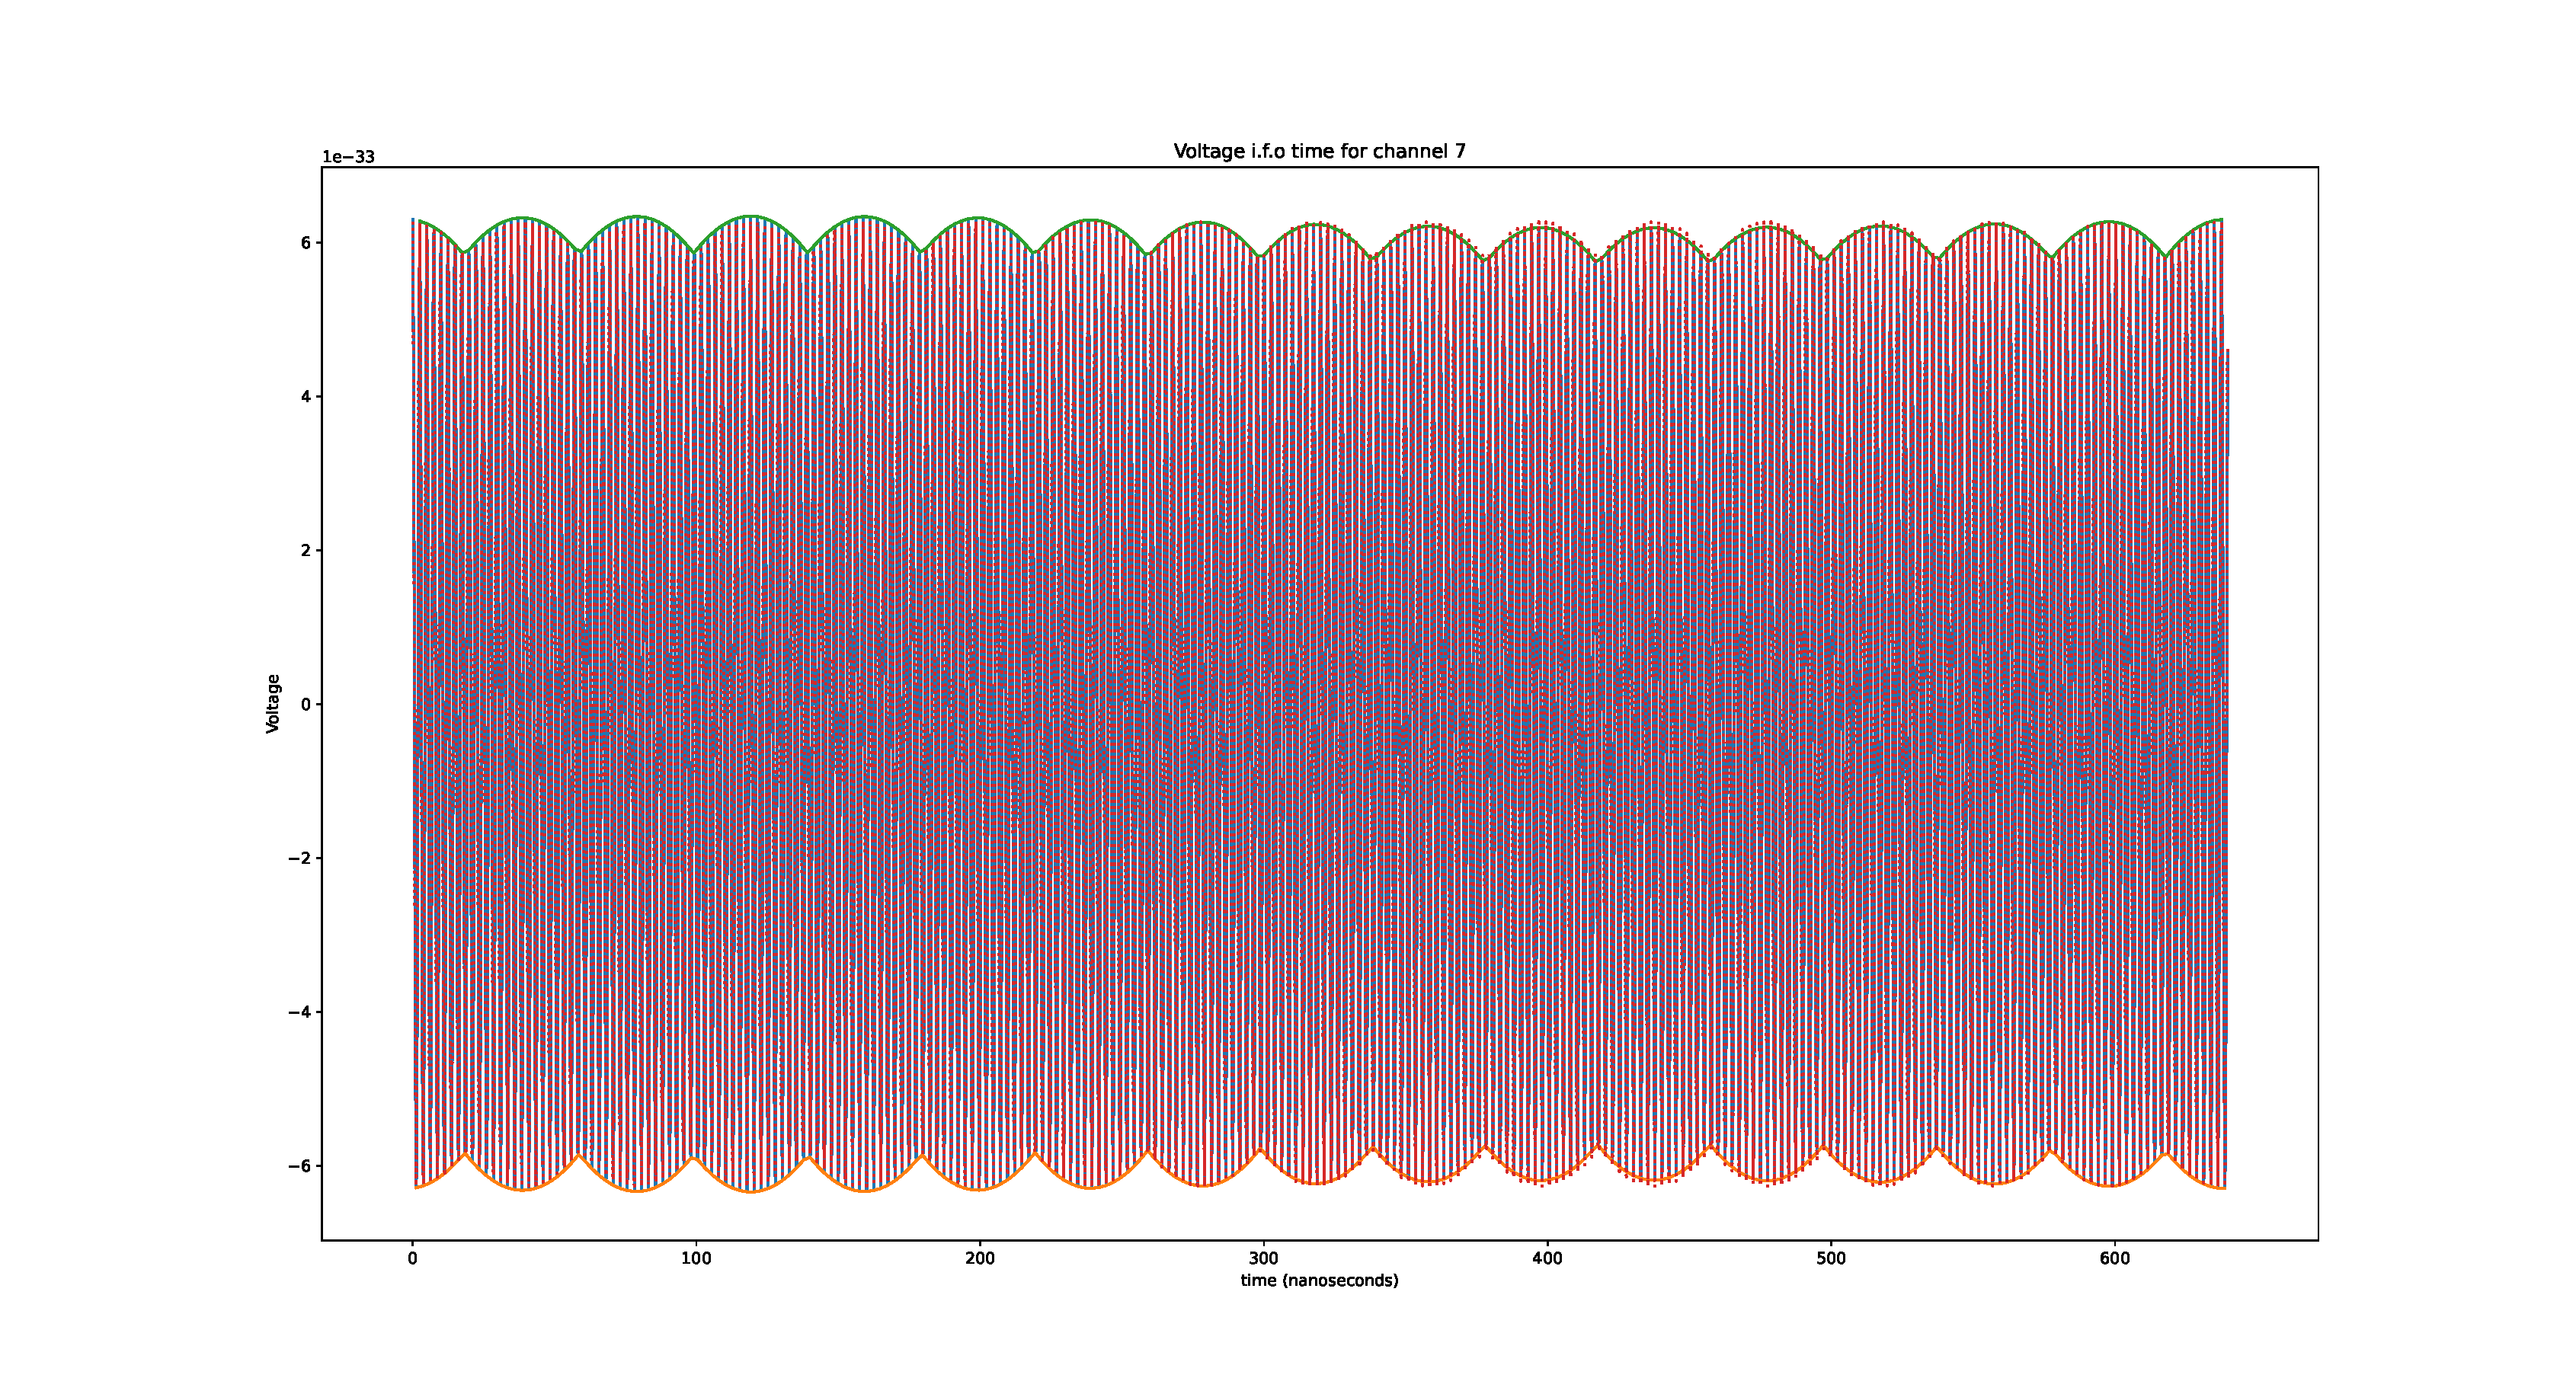
\includegraphics[width=\textwidth]{FitChannel7.pdf}
	\end{minipage}
	\caption{recorded voltage i.f.o time on detector 23 at 2022/08/29 11:18:32 for
	channels 6 and 7}
	\label{fig:FittedVoltage67}
\end{figure}
\subsection{Difference in timing}
The signals detected in the channels have the form 
\begin{align}
  V(t) &= \sin(\omega_c t + \phi_c)\left[1 + m\cos(\omega_m t + \phi_m)\right]\\
  &= \sin(\omega_c(t + \phi_c/\omega_c))\left[1 + m\cos(\omega_m( t + \phi_m/\omega_m))\right]\\
  &:= \sin(\omega_c(t + T_c))\left[1 + m\cos(\omega_m( t + T_m))\right]
\end{align}
Now, for the plane wave reconstruction, we want to know the difference between
the arrival times for channels 6 and 7.  We take it to be sufficient to let the
offset in time be the offset on the message as the offset on the carrier is 
sufficiently small, i.e
\begin{equation}
  \Delta T := T_6 - T_7 = T_6^m - T_7^m
\end{equation}
\begin{figure}
	\begin{minipage}{0.49\textwidth}
		\includegraphics[width=\textwidth]{ModulatedCh6.pdf}
	\end{minipage}
	\begin{minipage}{0.49\textwidth}
		\includegraphics[width=\textwidth]{ModulatedCh7.pdf}
	\end{minipage}
	\caption{recorded voltage i.f.o time on detector 23 at 2022/08/29 11:18:32 for
	channels 6 and 7}
	\label{fig:ModulatedChannels}
\end{figure}
our actual difference
in timing is thus:
\begin{equation}
	t_6 - t_7 = T_6 - T_7 - (t_6^d - t_7^d) = \Delta T - (t_6^d - t_7^d)
\end{equation}
Now going through the full calculation (i.e minimizing the correlation function
for different n given the time difference and finding the minimal distance
between reconstruction and balloon position)\footnote{Note that we used Snell's
law} we get that the index for refraction at a depth of 47.714m is 1.6061,
which is a fairly good estimate as, looking at the measurements depicted in
figure \ref{fig:DensityMeasurements} a depth of 47.7m would correspond to a
density of about $710 kg/m^3$, using Schytts equation this would thus give an
index of refraction of 1.603.  Now using the positional data we can calculate
the relative accuracy $\epsilon$ which comes to be about $0.39\%$. Our final
answer is thus:
\begin{table}[h]
    \centering
    \begin{tabular}{c|c|c|c|c|c}
      depth (m)& station number & run used & event\_id used & channels used & n\\
      \hline
      -47.714 & 23 & 691 & 489 & 6,7 & $1.606 \pm 0.006$
    \end{tabular}
\end{table}\\
Which has the expected answer within the margin of error. We are aware that this event 
also shows a peak in the frequency spectrum for channel 5 but the data deviates slightly
from an AM signal and thus didn't seem to be usable due to the difficulty of fitting it. 
\begin{figure}
  \centering
  \includegraphics[width=0.5\textwidth]{Frequencies.pdf}
  \caption{Frequencies sent out by the weather balloon}
  \label{fig:BalloonFreq}
\end{figure}
\newpage
\section{Fitting the index: deep components}
%\subsection{Station 24 run 646 event 373 Channels 0,1,2,3}
%Going through the full calculation again, i.e getting the relative balloon
%position and detector positions, fitting the AM function and thus finding the
%time offsets, minimizing the correlation function for every index of refraction
%n whilst recording the difference between the path and the weather balloon
%location and finally returning the index of refraction for which this
%difference is the smallest; we get as an index of refraction from fit at a
%depth of -96.1265m : 1.7648612972259445, if we now calculate the theoretical
%value (for a greenland simple ice model) of the \textit{relative accuracy}
%$\epsilon$ we get $3.369\%$. This thus implies a value of
%\begin{equation}
%  n = 1.765 \pm 0.059
%\end{equation}
%It is quite unfortunate that the uncertainty is that large.
%Now how does this compare to the expected value from density measurements?
%Looking at the density measurements shown in figure \ref{fig:DensityMeasurements} 
%we expect a density of about 860 $kg/m^3$ at a depth of 96.13m, using
%Schytt's equation with $\rho_0 = 917$ this implies an index of refraction of about 1.73
%which is within our confidence interval.

\subsection{Station 23 run 800 event 1867 Channels 0 and 3}
Using guesses $\phi_2^0 = -786.91$ \& $\phi_2^3 = -782$, traveltimes
[4822.41659697 4806.73065199] are found which have nearly the same difference
and size as the simulated [4822.16,4805.80]. The minimal correlation was found to be
$0.334$ns and yielded 1.7475 as index of refraction at a depth of -93.231m.
Epsilon is calculated to be 4.865\% for this Balloon position, our final result is 
thus:
\begin{table}[h]
    \centering
    \begin{tabular}{c|c|c|c|c|c}
      depth (m)& station number & run used & event\_id used & channels used & n\\
      \hline
      -93.231& 23 & 800 & 1867 & 0,3 & $1.748 \pm 0.085$
    \end{tabular}
\end{table}\\
From analysis of the density we expect an index of refraction of 1.73 which
lies inside our confidence interval.

\section{Special test: Channels 7 and 13}
\begin{table}[h]
    \centering
    \begin{tabular}{c|c|c|c|c|c}
      depth (m)& station number & run used & event\_id used & channels used & n\\
      \hline
      -19.11& 23 & 691 & 489 & 7,13 & $1.3777 \pm 0.117$
    \end{tabular}
\end{table}
This test isn't to be used as the error is too large but it might be useful
to know that a plane wave reconstruction with one of the nearest deep components and
a surface component is possible.

\chapter*{Conclusion}
\section*{Proposal of improved measurements}
As this method seems to be a viable way of measuring the index of refraction,
it might be a good idea to have a more controllable radio wave source fly
closer to the detectors to make more accurate measurements, e.g an
autonomous\footnote{as to not have it need a radio controller, causing RF interference 
and also as autonomous GNSS positioning are always more accurate than humans} drone with an
antenna strapped to it.  Assuming Schytt's equation to hold completely, ideally
we'd like data inbetween the depths of 20-100m as density measurements are few
there as depicted on figure \ref{fig:DensityMeasurements} which is possible to
achieve using this method as detectors span this range.

It would also help in the fitting of the AM signal is the message signal had a longer frequency
making it less difficult to fit.

\appendix
\chapter{List of abbreviations}
\begin{itemize}
\item \textbf{AM}: \textbf{A}mplitude \textbf{M}odulated
\item \textbf{CMB}: \textbf{C}osmic \textbf{M}icrowave \textbf{B}ackground
\item \textbf{DAQ}: \textbf{D}ata \textbf{AQ}uisition system
\item \textbf{DnR}: \textbf{D}irect a\textbf{N}d \textbf{R}efracted
\item \textbf{FFT} \textbf{F}ast \textbf{F}ourrier \textbf{T}ransform
\item \textbf{GRBs}: \textbf{G}amma-\textbf{R}ay \textbf{B}ursts
\item \textbf{RADIANT}: \textbf{RA}dio \textbf{DI}gitizer and \textbf{A}uxiliary \textbf{N}eutrino \textbf{T}rigger
\item \textbf{RNO-G}: \textbf{R}adio \textbf{N}eutrino \textbf{O}bservatory in \textbf{G}reenland
\item \textbf{UHE}: \textbf{U}ltra \textbf{H}igh \textbf{E}nergy 
\end{itemize}
\chapter{Balloon passbys under 5°\\ in the summer of 2022}
\label{app:5Deg}
\csvautotabular{tables/EventsBelow5DegPart1.csv}
\csvautotabular{tables/EventsBelow5DegPart2.csv}
\csvautotabular{tables/EventsBelow5DegPart3.csv}
\chapter{Balloon passbys under 10°\\ in the summer of 2022}
\label{app:10Deg}
\begin{table}[h!]
\csvautotabular{tables/EventsBelow10DegPart5.csv}
\end{table}
\begin{table}
\csvautotabular{tables/EventsBelow10DegPart1.csv}
\end{table}
\begin{table}
\csvautotabular{tables/EventsBelow10DegPart2.csv}
\end{table}
\begin{table}
\csvautotabular{tables/EventsBelow10DegPart3.csv}
\end{table}
\begin{table}
\csvautotabular{tables/EventsBelow10DegPart4.csv}
\end{table}

% =====================================================================
% End matter
% =====================================================================
\newpage
%----------------------------------------------------------------------------------------
%	REFERENCE LIST
%----------------------------------------------------------------------------------------
\bibliography{sources}
\bibliographystyle{plain}

\end{document}
